\documentclass[11pt, oneside, letter]{memoir}

% -----BEGIN PACKAGES-----
% Basic packages
\usepackage[T1]{fontenc}
\usepackage[margin=1in]{geometry}

% When adding a new package, add a comment briefly explaining why it is added
\usepackage{listings} % used for code formatting
\usepackage{blindtext} % filler text 
\usepackage{pdfpages} % insert PDFs into the document
\usepackage{todonotes} % \todo command
\usepackage{xspace} % \xspace command; not related to SpaceX ;)
\usepackage{subcaption} % subfigures
\usepackage{titlesec} % sexier section markers
\usepackage{amsmath} % \equation environment
\usepackage{tabulary} % better tables
\usepackage{longtable} % longer tables
\usepackage[hyphens]{url}
\usepackage[hidelinks,breaklinks]{hyperref} % toc has links
\usepackage{makecell} % \makecell command for multiline table cells
\usepackage[export]{adjustbox} % valign for alignment
\usepackage{xpatch} % to patch miscellanious commands manually
\usepackage{fancyhdr} % more advanced headers
\usepackage{tikz} % native charts
\usetikzlibrary{shapes,arrows,trees,calc} % tikz features
\usepackage{enumitem} % to allow customization of itemize and similar environments
\usepackage{mfirstuc} % title case automation
\usepackage{lastpage} % page number "of LASTPAGE"
\usepackage{float} % binding figures to sections etc
\usepackage{array} % array stretch to pad the tables and other table fun
\usepackage{supertabular} % headers on each page of longtables
\usepackage{color, colortbl} % color cells 
\usepackage{tablefootnote} % footnotes in tables
\usepackage{pdflscape} % landscape environment
\usepackage[ruled,vlined]{algorithm2e}
\usepackage[noend]{algorithmic} % also psuedocode
\usepackage{cite} % references
\usepackage{url} % url refs
\usepackage{subcaption}
\usepackage{graphicx}
% -----END PACKAGES-----

% -----BEGIN GLOBAL STYLE-----

% Misc config

% listings style
% Set up listings style
\definecolor{codegreen}{rgb}{0,0.6,0}
\definecolor{codegray}{rgb}{0.5,0.5,0.5}
\definecolor{codepurple}{rgb}{0.58,0,0.82}
% \definecolor{backcolour}{rgb}{0.95,0.95,0.92}
\definecolor{backcolour}{rgb}{255.0,255.0,255.0}

\lstdefinestyle{mystyle}{
    backgroundcolor=\color{backcolour},   
    commentstyle=\color{codegreen},
    keywordstyle=\color{magenta},
    numberstyle=\tiny\color{codegray},
    stringstyle=\color{codepurple},
    basicstyle=\ttfamily\footnotesize,
    breakatwhitespace=false,         
    breaklines=true,                 
    captionpos=b,                    
    keepspaces=true,                 
    numbers=left,                    
    numbersep=5pt,                  
    showspaces=false,                
    showstringspaces=false,
    showtabs=false,                  
    tabsize=2
}


\usepackage{fontspec}
\setmainfont{Droid Serif}
\setsansfont{Open Sans}
\openany % memoir layout
\xpatchcmd{\chapter}{\thispagestyle{chapter}}{}{}{} % chapter pages are formatted same as others
\xpatchcmd{\listoffigures}{\thispagestyle{chapter}}{}{}{} % chapter pages are formatted same as others
\renewcommand{\chaptername}{Section} % "Chapter" is only a logical tier, so call them sections
\maxtocdepth{subsection} % ToC uses subsection
\setsecnumdepth{subsection}

\renewcommand{\arraystretch}{1.5} % add a little bit more than standard padding to tables

% ToC
\renewcommand\contentsname{Table of Contents}
\renewcommand{\cftchapterfont}{\large\bfseries\sffamily}
\renewcommand{\cftchapterpagefont}{\large\bfseries\sffamily}
\renewcommand{\cftsectionfont}{\sffamily}  

% Header / footer
\pagestyle{fancy} % use fancyhdr
\addtocontents{toc}{\protect\thispagestyle{fancy}}
\addtocontents{lof}{\protect\thispagestyle{fancy}}
\addtocontents{lot}{\protect\thispagestyle{fancy}}
\lhead{\color{nu-purple}\sffamily\rightmark}
\rhead{\color{nu-purple}\sffamily\leftmark}
\lfoot{\color{nu-purple}\sffamily Rotor-Powered Rocket Lander}
\cfoot{\color{nu-purple}\sffamily}
\rfoot{\color{nu-purple}\sffamily\thepage\xspace} %of \pageref{LastPage}}
\renewcommand{\headrulewidth}{2pt}
\renewcommand{\headrule}{\hbox to\headwidth{%
    \color{nu-purple}\leaders\hrule height \headrulewidth\hfill}}
\renewcommand{\footrulewidth}{2pt}
\renewcommand{\footrule}{\hbox to\headwidth{%
    \color{nu-purple}\leaders\hrule height \headrulewidth\hfill}}

% Section line formatting
\titleformat{\chapter}[hang]
    {\Huge\sffamily\bfseries}
    {\thechapter\xspace{|}\xspace}
    {0pt}
    {\Huge\raggedright\bfseries}

% Special case for table of contents
\titleformat{name=\chapter,numberless}[hang]
    {\Huge\sffamily\bfseries}
    {\thechapter\xspace{|}\xspace}
    {0pt}
    {\Huge\raggedright\bfseries}

\titleformat{\section}[hang]
    {\LARGE\sffamily}
    {\thesection}
    {.5em}
    {}

\titleformat{\subsection}[hang]
    {\Large\sffamily\color{nu-purple}}
    {\thesubsection}
    {.5em}
    {}
    
\titleformat{\paragraph}
    {\sffamily\bfseries\color{nu-purple}}
    {}
    {0pt}
    {}
    
\titlespacing*{\paragraph}
    {0pt}
    {1em}
    {0.5em}
% -----END GLOBAL STYLE-----

% NUSTARS library
% -----BEGIN color textboxes-----
\usepackage{tcolorbox}
\usepackage{fontawesome}
\newcommand{\danger}[1]{
\begin{tcolorbox}[colback=red!5!white,colframe=red!75!black,title=\textbf{\faWarning\ EXTREME WARNING:}]
#1
\end{tcolorbox}}

\newcommand{\warn}[1]{
\begin{tcolorbox}[colback=orange!5!white,colframe=orange!95!black,title=\textbf{\faWarning\ WARNING:}]
#1
\end{tcolorbox}}

\newcommand{\caution}[1]{
\begin{tcolorbox}[colback=yellow!5!white,colframe=yellow!95!black,coltitle=black,title=\textbf{\faWarning\ CAUTION:}]
#1
\end{tcolorbox}}

\newcommand{\info}[1]{
\begin{tcolorbox}[colback=blue!5!white,colframe=blue!75!black,title=\textbf{\faInfoCircle\ INFO:}]
#1
\end{tcolorbox}}
% -----END color textboxes-----

% -----BEGIN color scheme-----
% NU branding; https://www.northwestern.edu/brand/visual-identity/color/index.html for more colors
\definecolor{nu-purple}{rgb}{0.306, 0.165, 0.518}
\definecolor{nu-purple-10}{rgb}{0.894, 0.878, 0.933}
\definecolor{nu-purple-160}{rgb}{0.1137, 0.00784, 0.20784}

% FMEA colors
\definecolor{fmea-red}{rgb}{1, 0.4, 0.4}
\definecolor{fmea-yellow}{rgb}{0.96, 0.96, 0.32}
\definecolor{fmea-green}{rgb}{0.32, 0.96, 0.35}

% -----END color scheme-----

% -----BEGIN NUSTARS environments-----
\newenvironment{ritemize}{\begin{itemize}[leftmargin=*]\raggedright}{\end{itemize}}

\usepackage{calc}
% Abstract full-width, equal width columns longtable
\newcommand{\nustarstable}[5]
{
    \begin{center}
    % TODO: locally redefine itemize->ritemize 
    % NOTE: the width needs to be less than 0.5 or it will overrun the right margin
    % TODO: the width needs to be dynamically calculated by the number of columns
    \begin{longtable}{|*{#1}{>{\raggedright\arraybackslash}m{.465\textwidth}|}}
    \caption{#4}
    \label{#5}
    \\\hline
    #2 \\\hline
    \endfirsthead
    %\bfseries #2 \\\hline % uncomment if we want headers on every page
    \endhead
    #3
    \\\hline
    \end{longtable}
    \end{center}
}

% Table with Requirement | Specification
% Intended to be used mainly for official NSL requirements
\newcommand{\requirements}[3]{\nustarstable
    {2}
    {\bfseries Requirement & \bfseries Specification}
    {#1}
    {#2}
    {#3}
}

% Table with Requirement | Justification
% Intended to be used for PDR only
\newcommand{\requirementsTeamPDR}[3]{\nustarstable
    {2}
    {\bfseries Requirement & \bfseries Justification}
    {#1}
    {#2}
    {#3}
}

% Table with Requirement | Justification | Verification
% Intended to be used for PDR only
\newcommand{\requirementsTeamCDR}[3]{\nustarstable
    {3}
    {\bfseries Requirement & \bfseries Justification & \bfseries Verification}
    {#1}
    {#2}
    {#3}
}

\newcommand{\itemizedBudget}[3]{
\begin{footnotesize}
\begin{longtable}{
|>{\raggedright\arraybackslash}p{.1\textwidth}
|>{\raggedright\arraybackslash}p{.075\textwidth}
|>{\raggedright\arraybackslash}p{.15\textwidth}
|>{\raggedleft\arraybackslash}p{.085\textwidth}
|>{\raggedleft\arraybackslash}p{.1\textwidth}
|>{\raggedleft\arraybackslash}p{.175\textwidth}
|>{\raggedleft\arraybackslash}p{.085\textwidth}
|>{\raggedleft\arraybackslash}p{.075\textwidth}
|}
    \caption{#2}
    \label{#3}
    \\\hline 
        \bfseries{Part} & \bfseries{Quantity} & \bfseries{Description} & \bfseries{Material} & \bfseries{Dimensions} & \bfseries{Part Number} & \bfseries{Supplier} & \bfseries{Cost}\\\endfirsthead
    \hline 
    #1
    \hline
    \end{longtable}
    \end{footnotesize}
    
}

\newcommand{\challenges}[3]{\nustarstable
    {2}
    {\bfseries Challenge & \bfseries Solution}
    {#1}
    {#2}
    {#3}
}

% FMEA cell codes
\newcommand{\oneA}{1A\cellcolor{fmea-red}}
\newcommand{\oneB}{1B\cellcolor{fmea-red}}
\newcommand{\oneC}{1C\cellcolor{fmea-red}}
\newcommand{\oneD}{1D\cellcolor{fmea-yellow}}
\newcommand{\oneE}{1E\cellcolor{fmea-yellow}}

\newcommand{\twoA}{2A\cellcolor{fmea-red}}
\newcommand{\twoB}{2B\cellcolor{fmea-red}}
\newcommand{\twoC}{2C\cellcolor{fmea-yellow}}
\newcommand{\twoD}{2D\cellcolor{fmea-yellow}}
\newcommand{\twoE}{2E\cellcolor{fmea-green}}

\newcommand{\threeA}{3A\cellcolor{fmea-red}}
\newcommand{\threeB}{3B\cellcolor{fmea-yellow}}
\newcommand{\threeC}{3C\cellcolor{fmea-yellow}}
\newcommand{\threeD}{3D\cellcolor{fmea-green}}
\newcommand{\threeE}{3E\cellcolor{fmea-green}}

\newcommand{\fourA}{4A\cellcolor{fmea-yellow}}
\newcommand{\fourB}{4B\cellcolor{fmea-yellow}}
\newcommand{\fourC}{4C\cellcolor{fmea-green}}
\newcommand{\fourD}{4D\cellcolor{fmea-green}}
\newcommand{\fourE}{4E\cellcolor{fmea-green}}

\newcommand{\priskHIGH}{High\cellcolor{fmea-red}}
\newcommand{\priskMED}{Medium\cellcolor{fmea-yellow}}
\newcommand{\priskLOW}{Low\cellcolor{fmea-green}}

\newcommand{\risks}[3]{
\begin{landscape}
\begin{footnotesize}
    \begin{longtable}{
    |>{\raggedright\arraybackslash}p{.15\textwidth}
    |>{\raggedright\arraybackslash}p{.2\textwidth}
    |>{\raggedright\arraybackslash}p{.2\textwidth}
    |>{\raggedright\arraybackslash}p{.09\textwidth}
    |>{\raggedright\arraybackslash}p{.25\textwidth}
    |>{\raggedright\arraybackslash}p{.09\textwidth}|}
    \endfirsthead
    \caption{#2}
    \label{#3}
    \\\hline 
        Risk & Cause & Effect(s) & Pre-RAC & Mitigation & Post-RAC \\
    \hline 
    #1
    \hline
    \end{longtable}
    \end{footnotesize}
\end{landscape}
}

\newcommand{\fmea}[3]{
\begin{landscape}
\begin{footnotesize}
    \begin{longtable}{
    |>{\raggedright\arraybackslash}p{.15\textwidth}
    |>{\raggedright\arraybackslash}p{.2\textwidth}
    |>{\raggedright\arraybackslash}p{.2\textwidth}
    |>{\raggedright\arraybackslash}p{.09\textwidth}
    |>{\raggedright\arraybackslash}p{.25\textwidth}
    |>{\raggedright\arraybackslash}p{.09\textwidth}|}
    \endfirsthead
    \caption{#2}
    \label{#3}
    \\\hline 
        Failure Mode & Cause & Effect(s) & Pre-RAC & Mitigation & Post-RAC \\
    \hline 
    #1
    \hline
    \end{longtable}
    \end{footnotesize}
\end{landscape}
}

\newcommand{\projectrisks}[3]{
\begin{landscape}
\begin{footnotesize}
    \begin{longtable}{
        |>{\raggedright\arraybackslash}p{.2\textwidth}
        |>{\raggedright\arraybackslash}p{.1\textwidth}
        |>{\raggedright\arraybackslash}p{.1\textwidth}
        |>{\raggedright\arraybackslash}p{.275\textwidth}
        |>{\raggedright\arraybackslash}p{.275\textwidth}
        |>{\raggedright\arraybackslash}p{.1\textwidth}|}
    \endfirsthead
    \caption{#2}
    \label{#3}
    \\\hline 
        Risk & Likelihood & Impact Value & Impact Description & Mitigation Description & Mitigation Impact\\ 
    \hline 
    #1
    \hline
    \end{longtable}
    \end{footnotesize}
\end{landscape}
}

% -----END NUSTARS environments-----

% Misc
\newcommand{\email}[1]{\color{nu-purple}\href{mailto:#1}{#1}\color{black}}

\begin{document}

\frontmatter


\begin{titlingpage}
% \begin{figure}[t]
%     \centering\includegraphics[width=\textwidth]{mccormick-logo.png}
% \end{figure}
\centering
\HUGE\color{nu-purple}\sffamily Rotor-Powered Rocket Lander \\
\vspace{1cm}
\Large\color{black}\sffamily June 9, 2022\\
\vspace{1cm}
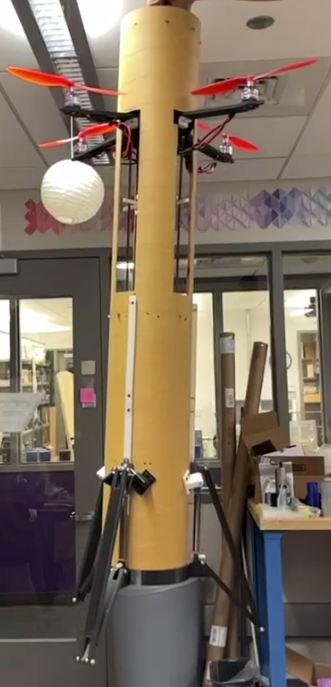
\includegraphics[width=0.28\textwidth]{src/figs/matt_holding_rocket.png}

\vspace{0.5cm}

\Large\color{black}\sffamily Submitted by:\\
\Large\color{gray}\sffamily Brooke Fujishima, Alexander Haws, Nicholas Marks,\\
Jorge Mena, David Michaels, Matthew Vinci\\

\vspace{1cm}
\Large\color{black}\sffamily Submitted to:\\
\Large\color{gray}\sffamily Sridhar Krishnaswamy \\
\vspace{1cm}

\Large\color{black}\sffamily Faculty Supervisors: \\
\Large\color{gray}\sffamily Michael Beltran, Alex Birdwell \\
\vspace{1cm}

\Large\color{black}\sffamily Sponsored by: \\
\Large\color{gray}\sffamily ME 398 Capstone Course - Mechanical Engineering Department\\
\vspace{1cm}
\end{titlingpage}

\renewcommand{\familydefault}{\sfdefault}
\tableofcontents*\clearpage
\listoffigures\clearpage
\listoftables\clearpage
% \listoftodos % REMOVE BEFORE SUBMISSION
\renewcommand{\familydefault}{\rmdefault}



% BODY OF REPORT
\mainmatter 
\chapter{Executive Summary}
On December 21, 2015, SpaceX accomplished one of the greatest feats in modern engineering history -- they successfully landed a first stage Falcon 9 booster after an orbital flight. Vertical takeoff, vertical landing (VTVL) technology has enabled humans to access space more rapidly, reliably, and affordably than ever before. Fittingly, the interest of VTVL boosters has also trickled down into the hobbyist rocketry community. Currently, there are hobbyist rockets that are able to land using a parachute; however, there is no design that takes advantage of rotors. Our client, Professor Sridhar Krishnaswamy, saw potential for innovation in this space and tasked us with building a VTVL rotor-powered rocket lander to broaden the capabilities of amateur rocketry.

The team identified two primary subsystems that were developed in parallel and merged into a final alpha prototype. The controls subteam was responsible for detecting drop, generating thrust, flight controls, deployment controls, and stabilization. The structures subteam designed the accompanying hardware to support mounting, actuation, deployment, and landing of the system. 

The controls subteam built a drone from scratch using a Raspberry Pi as the flight computer and a Pixhawk microcontroller as the flight controller. In conjunction, they are able to delegate commands and stabilize the drone. The team heavily relied on ArduPilot, an open-source drone control and stabilization library which was communicated with through an open-source python library called DroneKit. The robustness, customization, and plug-and-play nature of these systems lent themselves well to integration with structural components down the line.

The structures subteam was responsible for selecting a rocket body, developing a reusable and maintainable core assembly, and designing stowed and deployed locking mechanism for the in-house developed motor arms and landing legs. Due to the large number of components and systems being developed concurrently throughout the project, the design process was highly iterative and testing oriented. 

The alpha prototype is a 41 inch tall and 6 inch in diameter phenolic cardboard rocket tube with an internal core structure that securely houses and facilitates actuation of all deployable components. With a 1.25 thrust-to-weight ratio and a deployment time of 0.8 seconds, the lander would require 15.68m of drop height to achieve hover and it was deemed unsafe to test with current facility limitations. The final prototype is capable of detecting drop and deploying arms and legs. All electronic hardware and control software exist to achieve stable landing.

This report is a technical summary of the design decisions, analysis, and testing performed to achieve the alpha prototype. After reading this report, one should feel comfortable replicating the work that has been done in a more efficient manner, and making necessary improvements to achieve a successful landing. 

\chapter{Problem \& Background}

As discussed in the executive summary, the purpose of this project is to investigate and build a scaled down VTVL rocket which uses rotors and propellers to generate thrust for landing rather than a combustible fuel. The rotor arms and landing legs must be deployable during landing to accommodate a hypothetical launch scenario where the rocket was coming back to the ground and be guided to a landing pad.

One of the intended applications of this design is the NASA Student Launch Competition (NSL), which is an annual collegiate rocketry competition. The Northwestern Space Technology and Rocketry Society (NUSTARS) participates in this competition each year. Competition criteria change yearly; however, there are unvarying rules that follow national flight regulations. One important criterion prohibits the use of combustion fuel thrusters following initial ascent. This project will therefore be constrained following NSL’s competition rules so that NUSTARS can use this developed technology in the future. 

Our client, Professor Sridhar Krishnaswamy, was motivated to pursue this project based on the ongoing development by aerospace companies to create commercial and reusable rockets. In particular, the safe landing of aerospace vehicles in urban environments. Thus, another aim of this project is to investigate scaled down technologies that could theoretically aid in safely returning humans from extraterrestrial missions.

The scope of the project includes initial acceleration due to free fall, deployment of propulsion to slow down the vehicle, deployment of landing gear to land the vehicle upright, and controlled navigation to a desired landing zone. However, in our new new storyboard, we highlight the aspects of the project that we achieved, along with a potential step of hitting a hover, which we believe that we could accomplish quickly with the proper safety equipment. Hitting a hover would allow the rocket to behave in a manner similar to a quad copter, making the landing process easier. This storyboard is shown is figure \ref{fig:storyboard}.

\begin{figure}
    \centering
    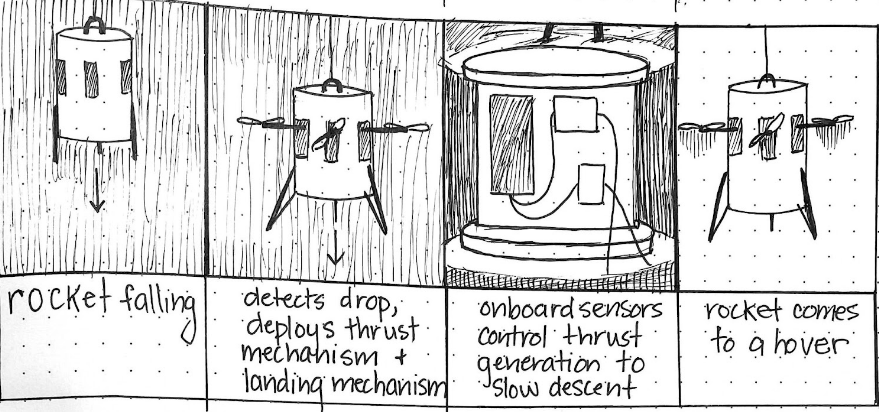
\includegraphics[width = 0.5\textwidth]{src/figs/Storyboard.png}
    \caption{New Updated Storyboard}
    \label{fig:storyboard}
\end{figure}

%MISSION STATEMENT
\clearpage
\section{Mission statement}
Our project seeks to develop a scaled rocket landing system capable of landing a rocket
vertically on a movable landing pad, while adhering to requirements set forth by NASA’s
Student Launch Competition, to broaden capabilities of rocket re-usability and missions.

\chapter{Competitive Analysis, IP, \& Benchmarking}
\label{competitive-analysis}
Rockets are inherently expensive machines. Up until SpaceX's landing of it's Falcon 9 boosters (see \cite{spacex-website}), the first stages of rockets were one-time-use machines. They were either expelled into the ocean during launch or incinerated by the atmosphere upon an unprotected re-entry. Making the first stage reusable has slashed launch costs while increasing launch cadence. An image of the Saturn 5 Engine in the ocean is shown in figure \ref{fig:S5E}.

\begin{figure}[H]
    \centering
    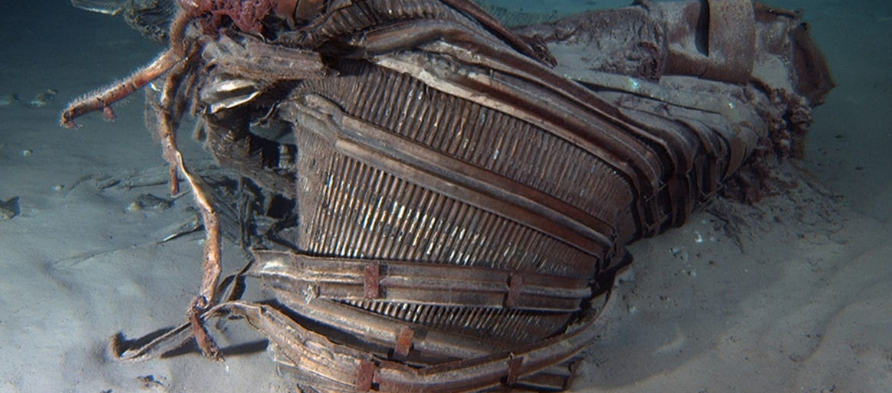
\includegraphics[scale=0.5]{src/figs/Saturn5_In_Ocean.png}
    \caption{Saturn 5 Engine in the Deep Sea}
    \label{fig:S5E}
\end{figure}

Making a rocket reusable is only advantageous if the combined cost of launching and refurbishing the associated landing mechanisms and flight hardware is less than the cost of building an entirely new rocket. We estimate that a landing system which weighs 20 percent of the rocket's wet mass would be on par with the current industry status quo. 

\section{Current Solutions to the Problem}

\subsection{Solutions to the Large Scale Problem}

At the date of writing this report, SpaceX and Blue Origin are the only two companies who have successfully developed orbital rockets that are capable of vertical takeoff and vertical landing (VTVL). Please refer to the following subsections for an in-depth technical analysis of these solutions.

\paragraph{SpaceX}
The Falcon 9 is a best-in-class two-stage rocket designed to carry payload and astronauts to a wide range of orbits and planets. They are powered by nine Merlin engines, hence the name, which generate in excess of 1.7 million pounds of thrust at sea level. These capable engines are fueled by cryogenically cooled liquid-oxygen (LOX) and rocket-grade kerosene (RP-1). All nine engines are equipped with two-axis gimballing mechanics to provide thrust-vectoring control of roll, pitch, and yaw upon ascent and landing. These engines are shown in figure \ref{fig:MEngine}.

\begin{figure}[H]
    \centering
    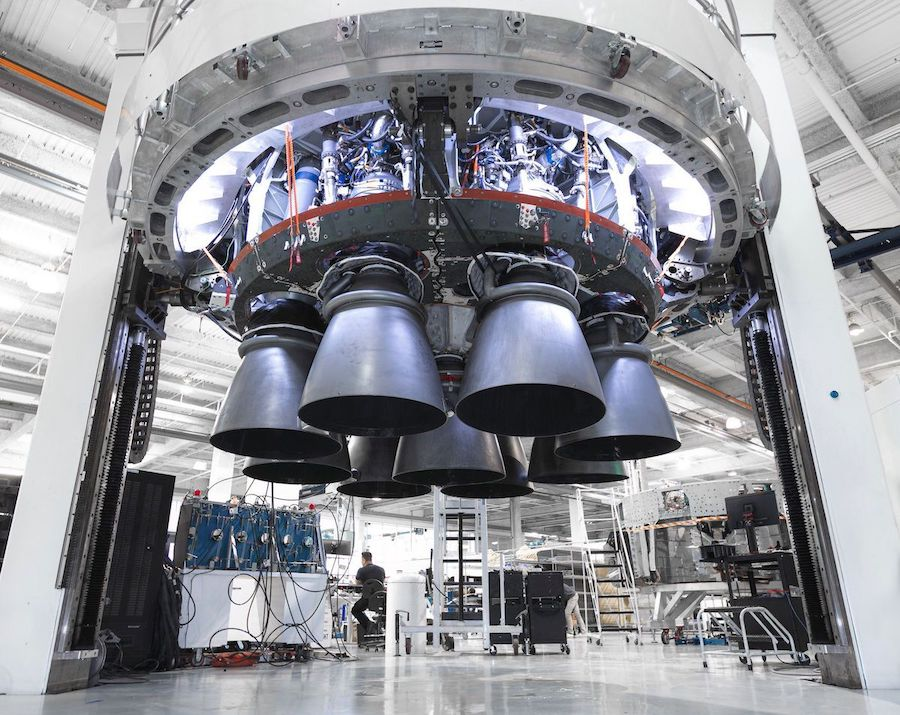
\includegraphics[scale=0.35]{src/figs/MerlinEngine.jpg}
    \caption{Merlin Engine}
    \label{fig:MEngine}
\end{figure}

Upon reaching apogee, the first stage of the rocket re-orients itself for return to earth. Cast titanium grid fins serve as actuating control surfaces to vertically orient and stabilize descent of the first stage through Earth's upper and lower atmosphere (figure \ref{fig:GFs}). The rocket navigates to its landing pad or a sea-fairing drone ship before performing a final landing burn, deploying landing legs, and making a successful touch-down back on Earth. (Figure \ref{fig:Fal9})

\begin{figure}[H]
    \centering
    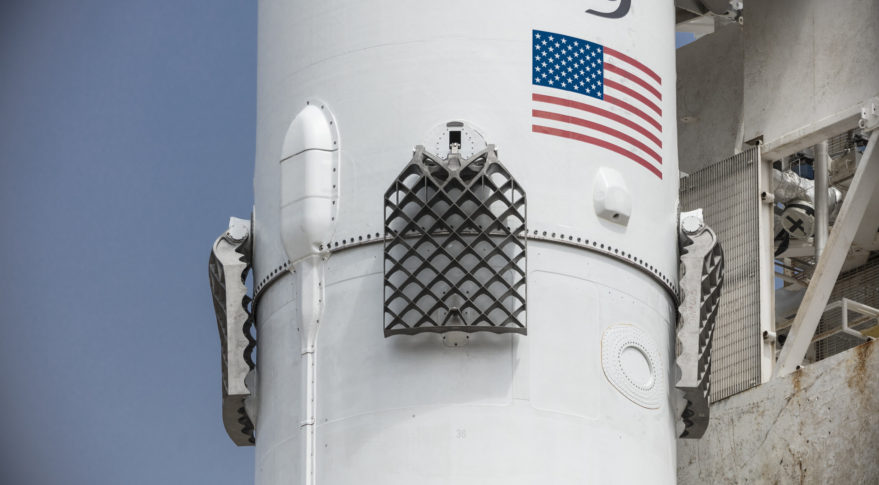
\includegraphics[scale=0.3]{src/figs/GridFins.jpg}
    \caption{Grid Fins}
    \label{fig:GFs}
\end{figure}

\begin{figure}[H]
    \centering
    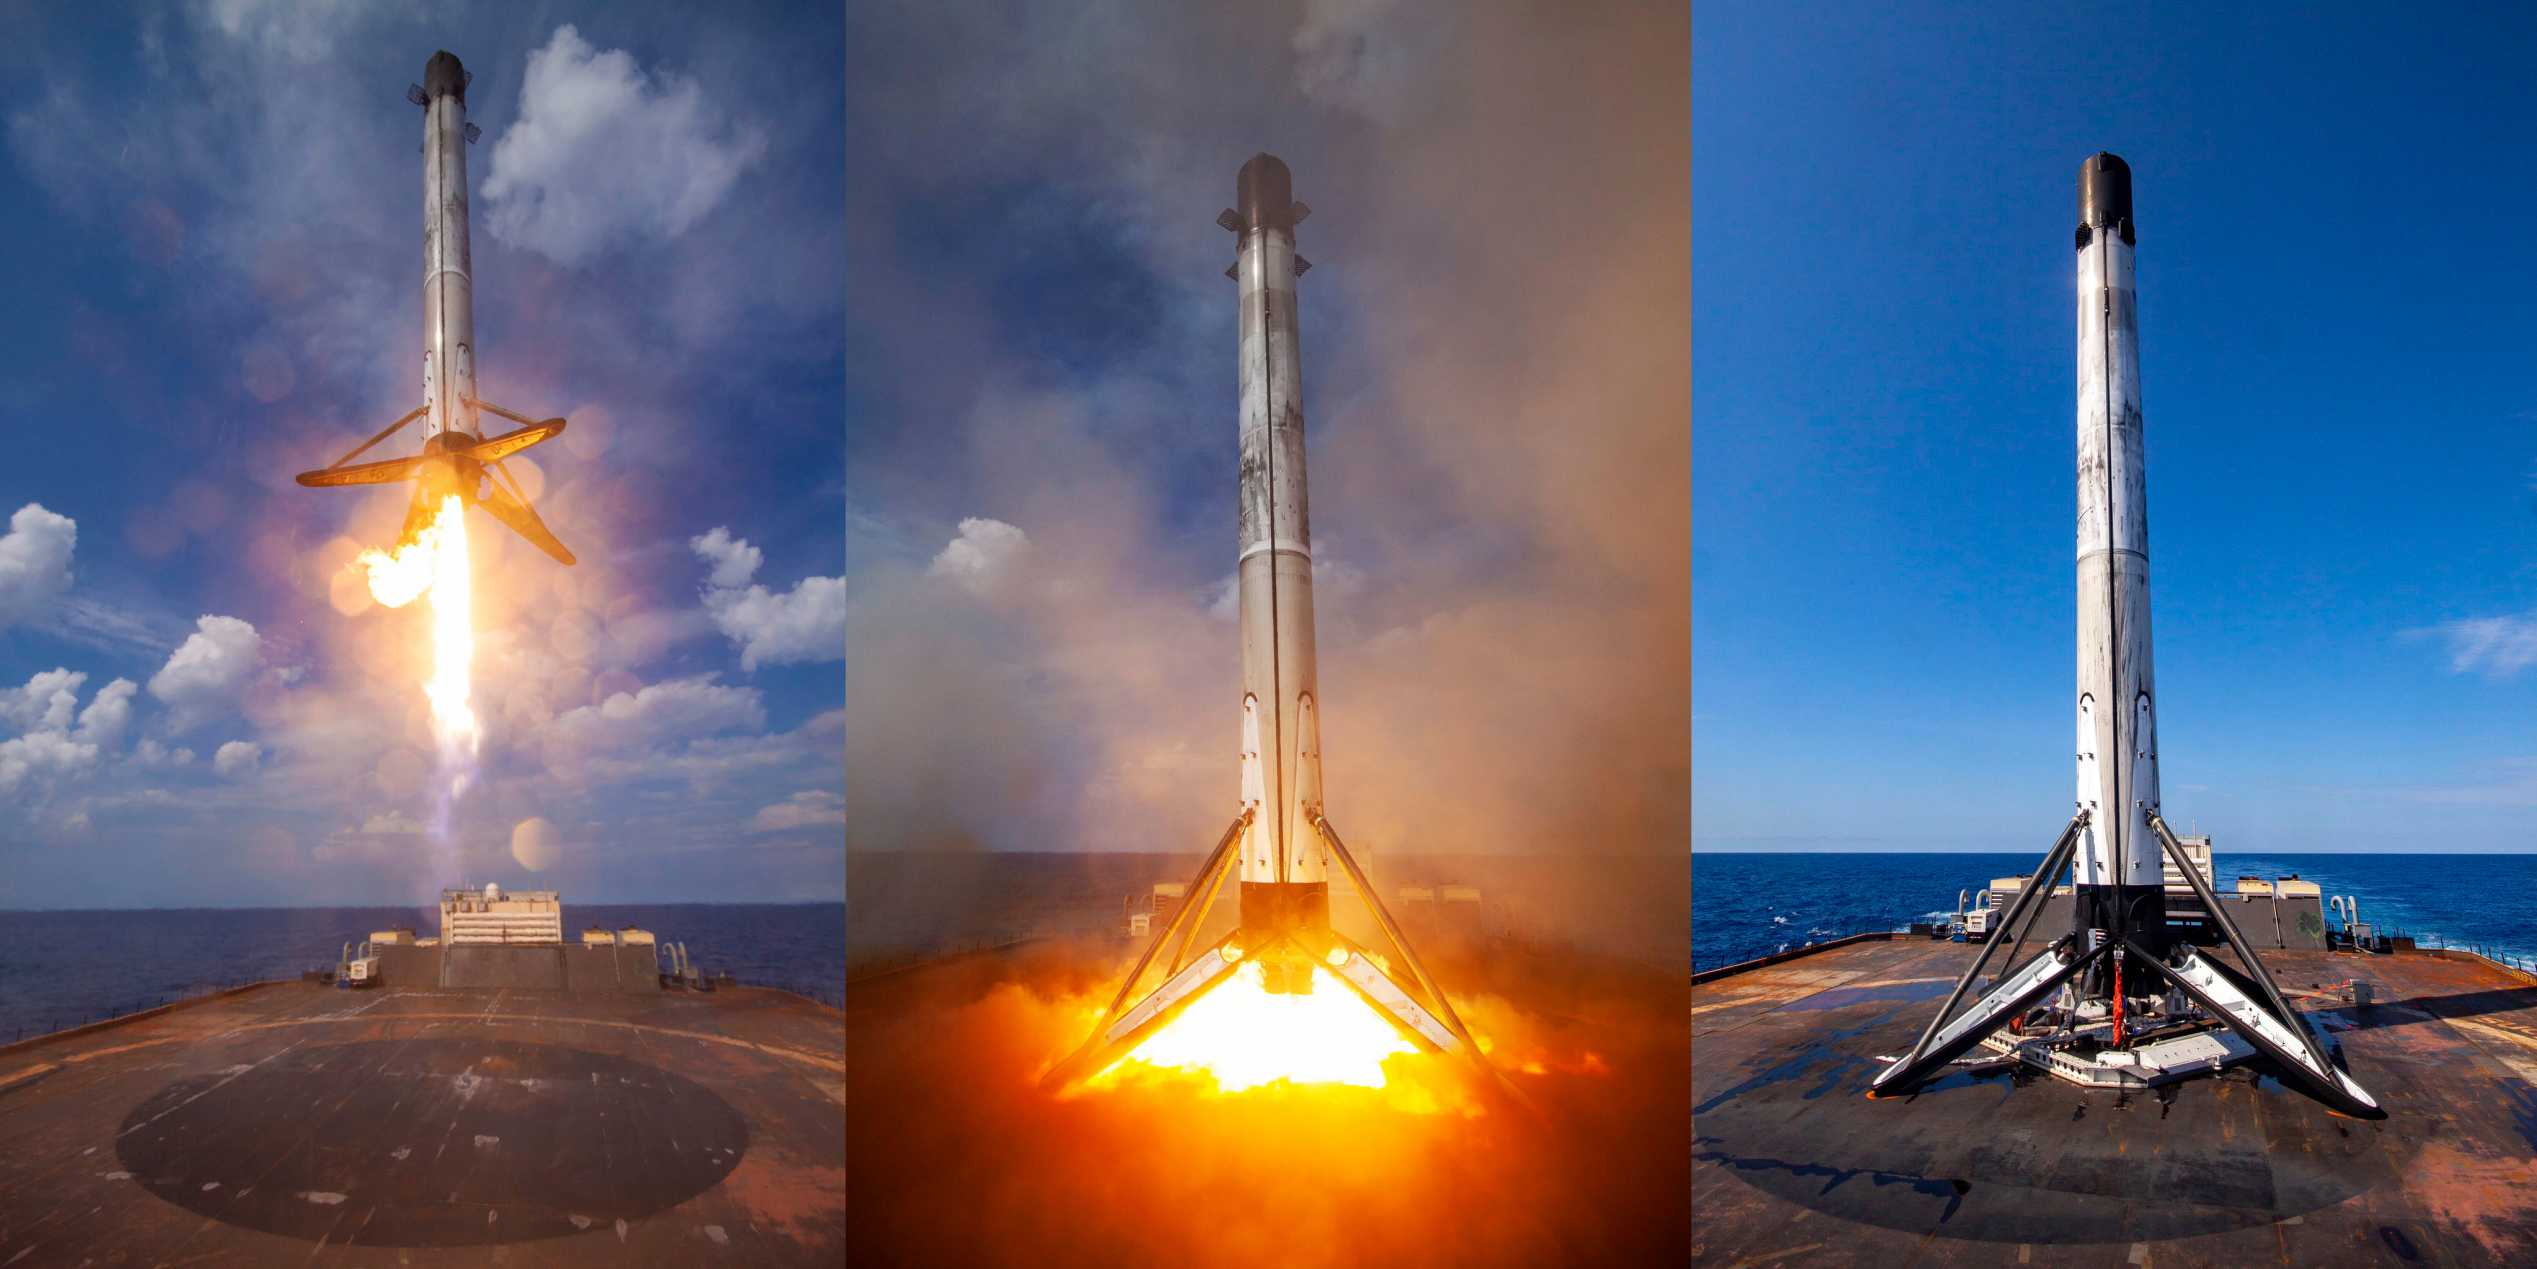
\includegraphics[scale=0.4]{src/figs/Falcon9_Landed.jpg}
    \caption{Falcon 9 Landing Stages}
    \label{fig:Fal9}
\end{figure}

SpaceX is also developing a heavy-lift vehicle named Starship capable of vertical takeoff and vertical landing (\ref{Starship}). Starship is an engineering marvel which will be capable of bringing 100+ tons of cargo to LEO with it's sights set on bringing humans and cargo to Mars.

\begin{figure}[H]
    \centering
    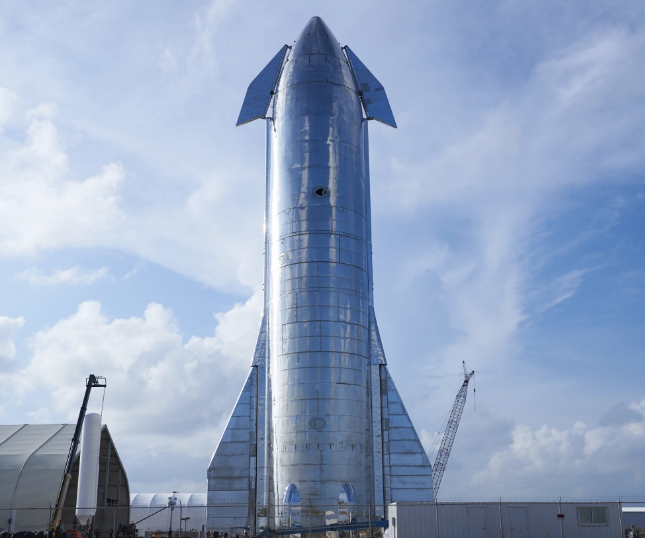
\includegraphics[scale = 0.7]{src/figs/Starship_2.png}
    \caption{SpaceX's Starship}
    \label{fig:Starship}
\end{figure}

In contrast to the Falcon 9, Starship will a staggering 33 Raptor 2 engines capable of generating 500,000 pounds of thrust a piece. Raptor engines are fueled by LOX and liquefied natural gas (LNG) which is primarily composed of methane. Liquid methane can be synthesized using the Sabatier reaction which can be produced on the surface of Mars to allow for on-planet refueling and return to Earth. 

SpaceX has openly announced plans to 'catch' the Super Heavy first stage of Starship using a ground based tower (figure \ref{fig:CTower}). Similar to Falcon 9, Super Heavy will re-orient and navigate itself using a similar gridfin and gimballing motor combination upon it's descent to the catch tower. This will eliminate the need for heavy landing legs which will cut mass and enable faster turn-around between launches.

\begin{figure}[H]
    \centering
    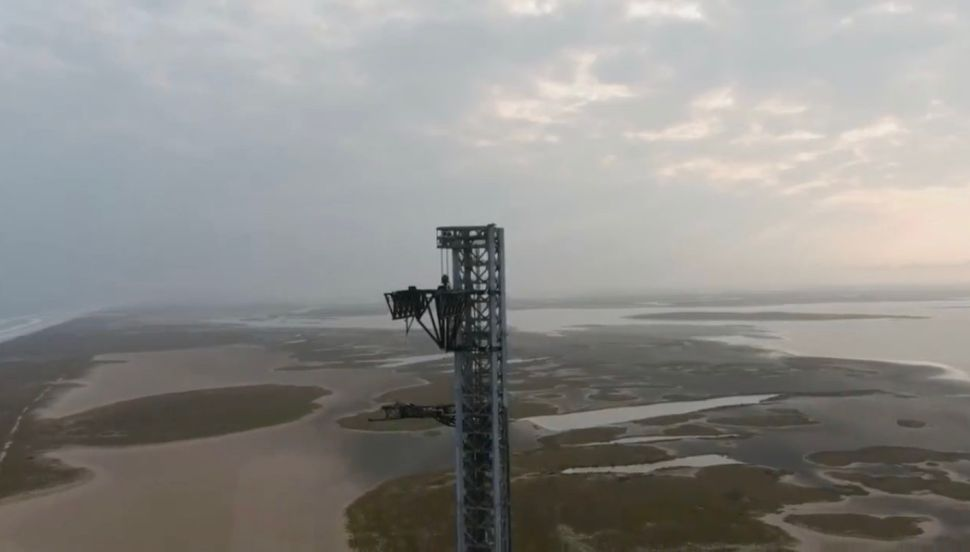
\includegraphics[scale = 0.4]{src/figs/CatchTower.jpg}
    \caption{Catch Tower}
    \label{fig:CTower}
\end{figure}

\paragraph{Blue Origin}

Currently, the only other rocket capable of a VTVL landing is Blue Origin's New Shepard \cite{blue-origin-website}. (Figure \ref{fig:BO}). Designed to tap into the budding space tourism market, this rocket can carry 6 passengers past the Karman Line on an eleven minute joy ride. 

\begin{figure}[H]
    \centering
    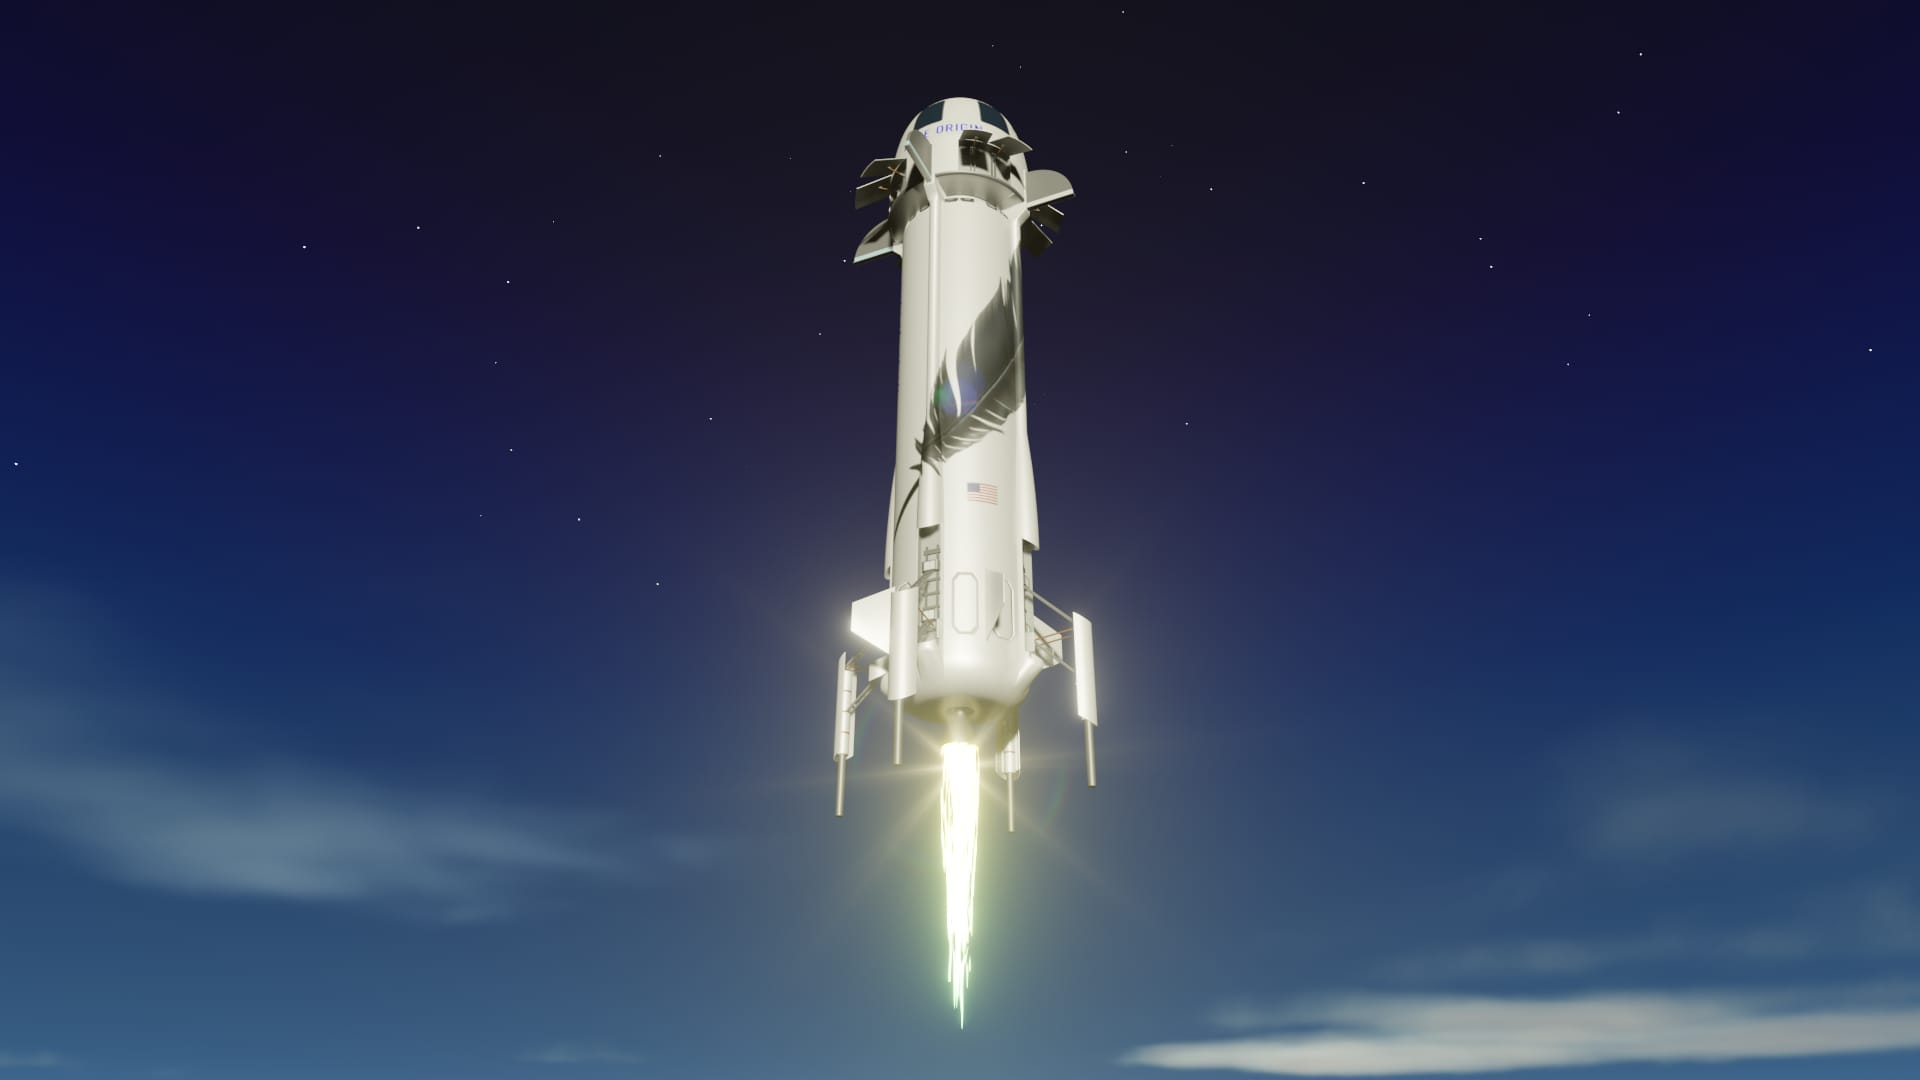
\includegraphics[scale=0.20]{src/figs/NewShepard2.jpg}
    \caption{New Shepard}
    \label{fig:BO}
\end{figure}

While the crew capsule makes its parachuted descent back to Earth, the New Shepard rocket lands at a remote pad. It is powered by a singular Blue Origin BE-3 engine which burns LOX and liquid hydrogen (Figure \ref{fig:BE3}). BE-3's are capable of producing 490 kN of thrust at sea level and are also equipped with gimballing mechanics. New Shepard utilizes drag brakes and aft fins for return stabilization through Earth's upper and lower atmosphere. 

\begin{figure}[H]
    \centering
    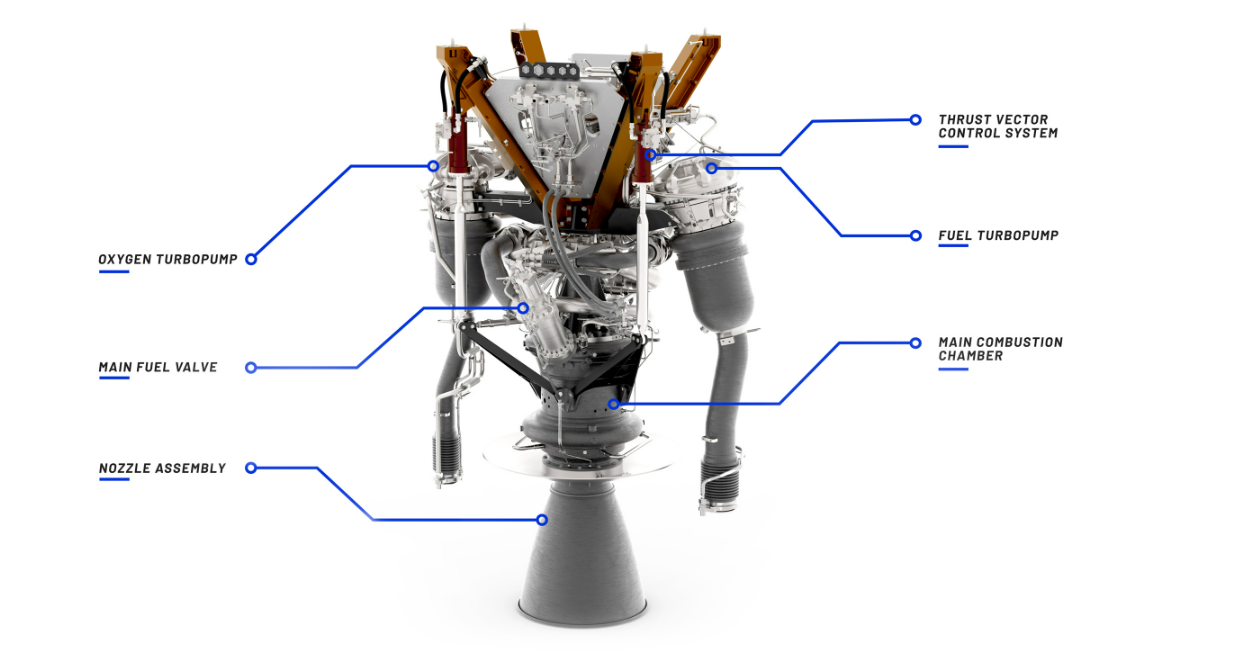
\includegraphics[scale = 0.5]{src/figs/BE-3_Engine.png}
    \caption{BE-3 Engine}
    \label{fig:BE3}
\end{figure}

Blue Origin is also developing a heavy-lift vehicle named New Glenn (Figure \ref{fig:NGR}). However, a fully functional prototype has not been produced. This rocket will be nearly 100 m tall and will use a new BE-4 Engine

\begin{figure}[H]
    \centering
    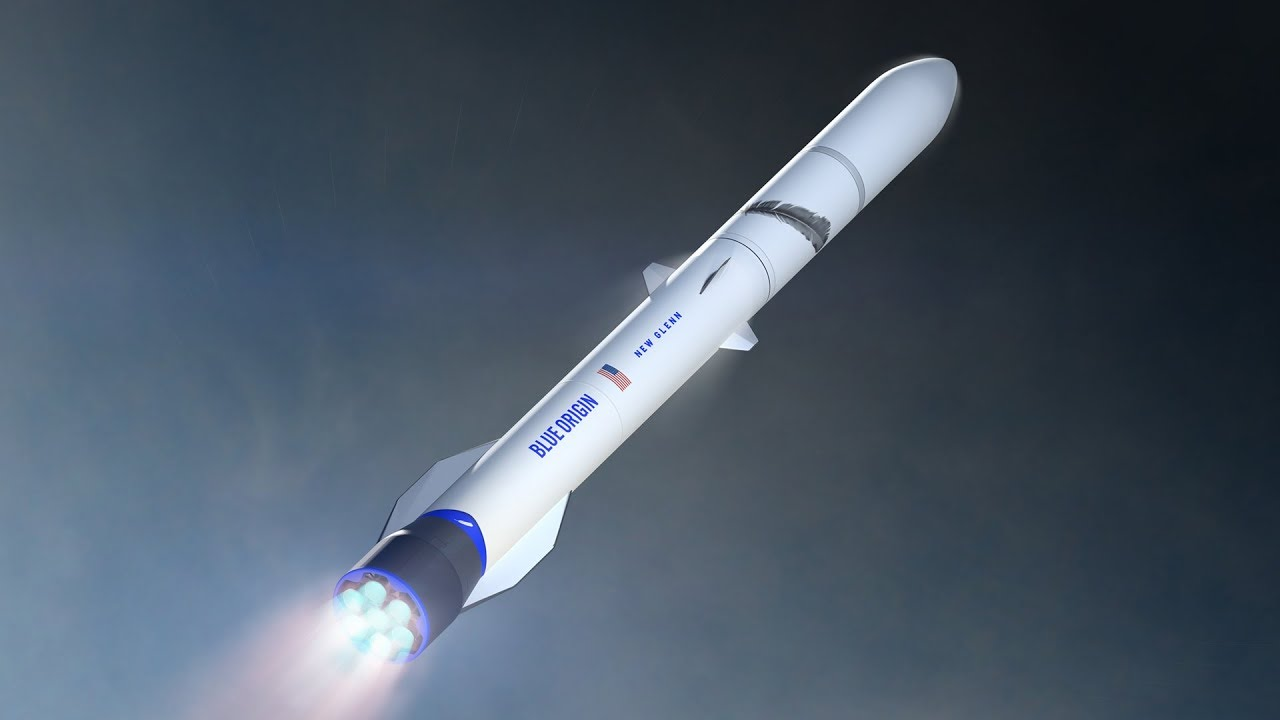
\includegraphics[scale = 0.3]{src/figs/NewGlenn.jpg}
    \caption{New Glenn Rocket}
    \label{fig:NGR}
\end{figure}

\subsection{Current Tech in the Hobby Rocketry Community}

As mentioned in the Executive Summary, VTVL rockets have begun to make their debut in the hobbyist rocketry scene as well. His Scout rocket flying is shown in figure \ref{fig:SR}. While a successful landing has yet to be achieved, a promising candidate is the Scout rocket being designed, manufactured, and tested by the incredible Joe Barnard at BPS.Space \cite{bps-space-website}. 

\begin{figure}[H]
    \centering
    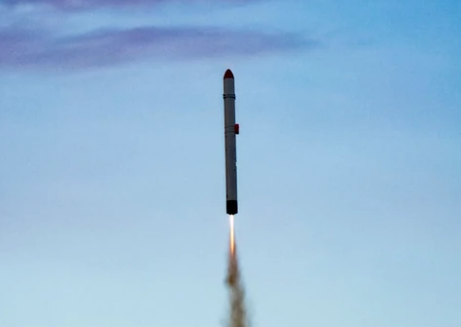
\includegraphics{src/figs/Scout_rocket.png}
    \caption{Scout Rocket}
    \label{fig:SR}
\end{figure}

Barnard has pioneered thrust vectoring and throttle modulation of solid-propellant rockets to the hobbyist scene. He sells a 3D printed gimbal paired with an in-house avionics board and software. Images of an attempted landing and the gimbal are shown in \ref{fig:HL} and \ref{fig:gimbal}, respectively. 

\begin{figure}[H]
    \centering
    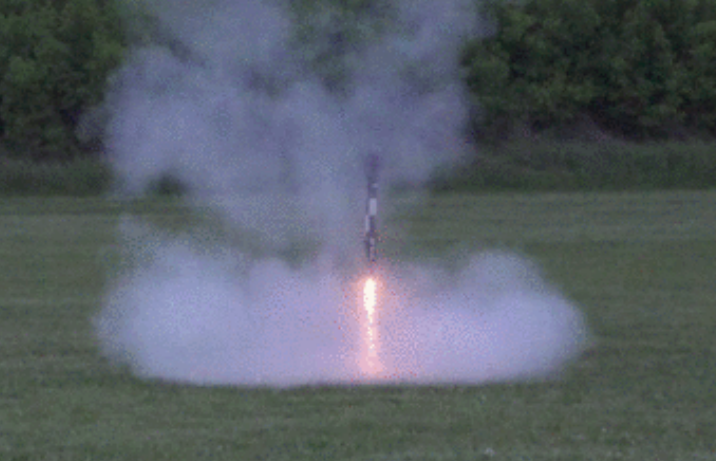
\includegraphics[scale=0.5]{src/figs/HobbyLander.png}
    \caption{Hobby Lander}
    \label{fig:HL}
\end{figure}


\begin{figure}[H]
    \centering
    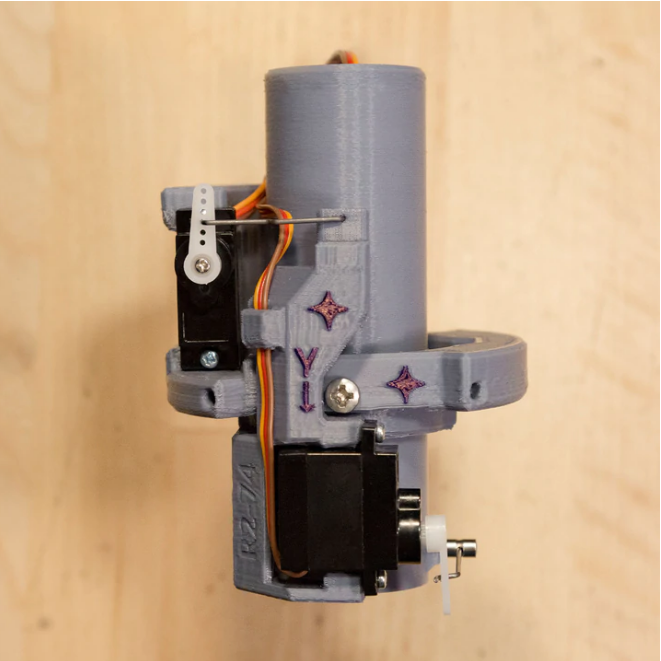
\includegraphics[scale=0.5]{src/figs/gimball.png}
    \caption{Gimbal of Hobby Rocket Engine}
    \label{fig:gimbal}
\end{figure}

\section{Relevant Patents}

The relevant patents to this project are shown below in figures \ref{fig:P1} through \ref{fig:P6}. They are broken up into categories of patents on landing processes and landing components.

\subsection{Patents on Landing Processes}

\paragraph{Launch vehicle with engine mounted on a rotor: US5842665A}
\begin{itemize}
    \item Launch vehicle has four bladed rotor mounted onto the body.
    \item Vehicle Body has propellant tanks and a payload compartment contained with an aeroshell.
    \item Engines connected by propellant feed lines to a transfer hub around the rotor axis of rotation.
\end{itemize}

\begin{figure}[H]
    \centering
    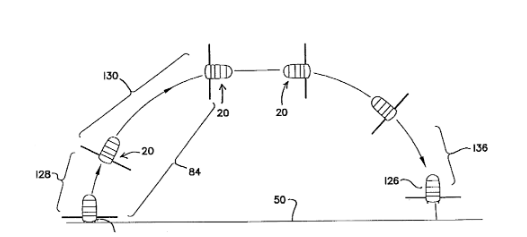
\includegraphics{src/figs/Patent1.png}
    \caption{Rotor Launch Vehicle Patent}
    \label{fig:P1}
\end{figure}


\paragraph{Convertible Vertical Take-off and Landing Miniature Aerial Vehicle: US6502787B1}
\begin{itemize}
    \item Take-off and Landing Vehicle which extends with an upper fuselage segment and a lower fuselage segment extending in opposite directions.
    \item Rotor rotates within a rotor guard assembly between the fuselage segments.
    \item Plural grin fins extend radially from the lower fuselage segment under the turning vanes.
\end{itemize}

\begin{figure}[H]
    \centering
    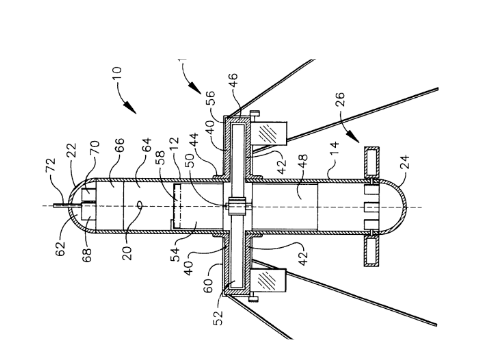
\includegraphics{src/figs/Patent2.png}
    \caption{Convertible Take-off and Landing Miniature Aerial Vehicle}
    \label{fig:P2}
\end{figure}

\subsection{Patents on Landing Components}

\paragraph{Curved Grid Fin: US5048773A}
\begin{itemize}
    \item Curved grid fin made of strips of gauge metal secured together in a honeycomb grid pattern structure.
    \item Base structure secured to a support structure which provides a fin designed to be mounted onto a missile.
    \item Can control or guide a missile as well as provide deceleration.
\end{itemize}

\begin{figure}[H]
    \centering
    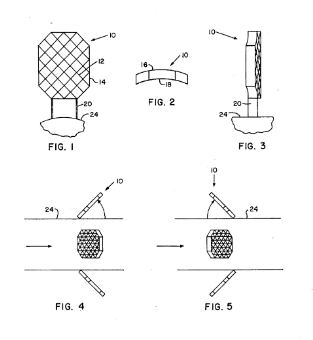
\includegraphics{src/figs/Patent3.png}
    \caption{Curved Grid Fin}
    \label{fig:P3}
\end{figure}

\paragraph{Landing gear for spacecraft: US8413927B2}
\begin{itemize}
    \item Pivotal connection and disrupt-able mechanical connection mount to a football on a distal end of landing legs.
    \item Sensor elements to respond to landing procedures and breaking points.
    \item When the foot-pad makes contact, mechanical connection breaks at rated breaking point, leading to sensors providing signal to turn off retro-thrusters.
\end{itemize}

\begin{figure}[H]
    \centering
    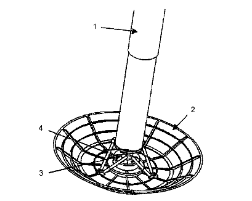
\includegraphics{src/figs/Patent5.png}
    \caption{Landing Gear for Spacecraft}
    \label{fig:P5}
\end{figure}

\paragraph{Adjustable landing gear assembly for unmanned aerial vehicles: US9592908B2}
\begin{itemize}
    \item Using telescoping legs to land the aerial vehicle while also adjusting to uneven ground.
    \item Legs can be retracted to fit to the inside of the vehicle.
\end{itemize}


\begin{figure}[H]
    \centering
    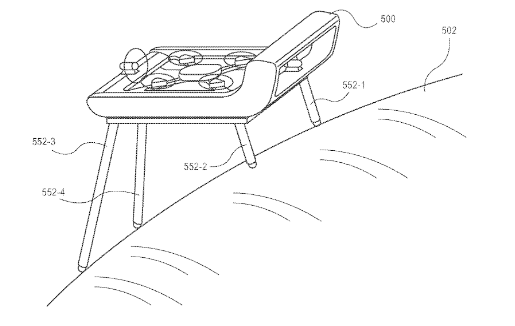
\includegraphics{src/figs/Patent6.png}
    \caption{Adjustable Landing Gear Assembly}
    \label{fig:P6}
\end{figure}


\chapter{Needs, Requirements, \& Specifications}
\label{needs-and-specs}
The project needs encapsulate specific components of the project that the final prototype must accomplish in order to be successful. The needs table was developed from the initial project statement provided by our client and was further iterated on after subsequent meetings with him and the team’s research. 
An important need that was identified was the safety of the team. After the main development of the final prototype it was found that dropping the vehicle into free-fall from a height of 10 m contained risks that we did not have the infrastructure to mitigate. Some of these risks include failure of rotor deployment, failure to control the motion of the vehicle, fracturing of components and subsequent ballistic fragment motion, and the destruction of the vehicle. Instead of performing the functions of the prototype all together with a drop test, the team focused on a safer alternative that would aim at testing each individual mechanism within a controlled environment. Figures \ref{needs-table} and \ref{needs-limits-table} show the needs that the team identified and the metrics that are used to test the functionality of the design.

\begin{figure}
    \centering
    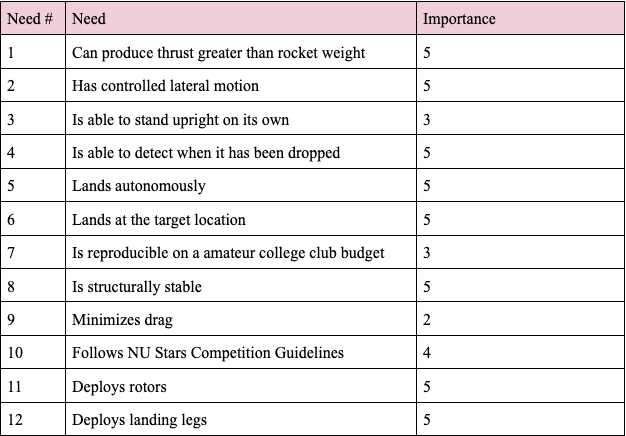
\includegraphics[width=1.0\textwidth]{src/figs/needstable.png}
    \caption{Design Needs \\ *Importance ranked on a scale from 1-5, where 5 is the highest}
    \label{needs-table}
\end{figure}


\begin{figure}
    \centering
    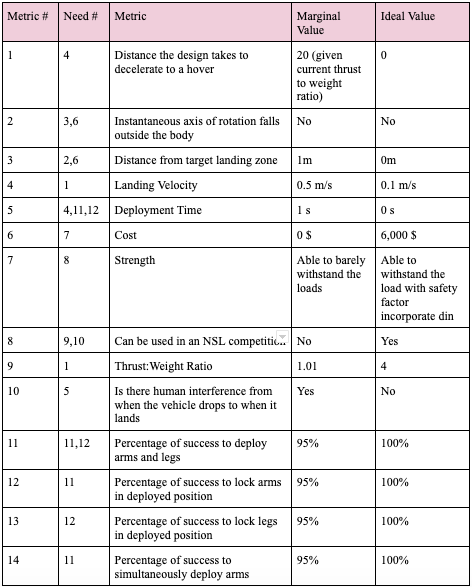
\includegraphics[width=1.0\textwidth]{src/figs/metricstable.png}
    \caption{Acceptable Limits for Metrics}
    \label{needs-limits-table}
\end{figure}
\chapter{Product Architecture}

\section{Systems Overview} 
The alpha prototype is composed of three major systems: the propulsion arm system, the landing leg system and the control electronics system. The 3 main systems work in unison to transform an amateur rocket into a full fledged autonomous landing system capable of deploying the necessary components and safely landing the rocket. Each of these primary systems is composed of an array of smaller components that work in unison to perform the systems required tasks for safe landing. A full CAD assembly of the final design without the upper airframe is shown in Figure \ref{arch:full-cad:labelled}
\begin{figure}[H]
    \centering
    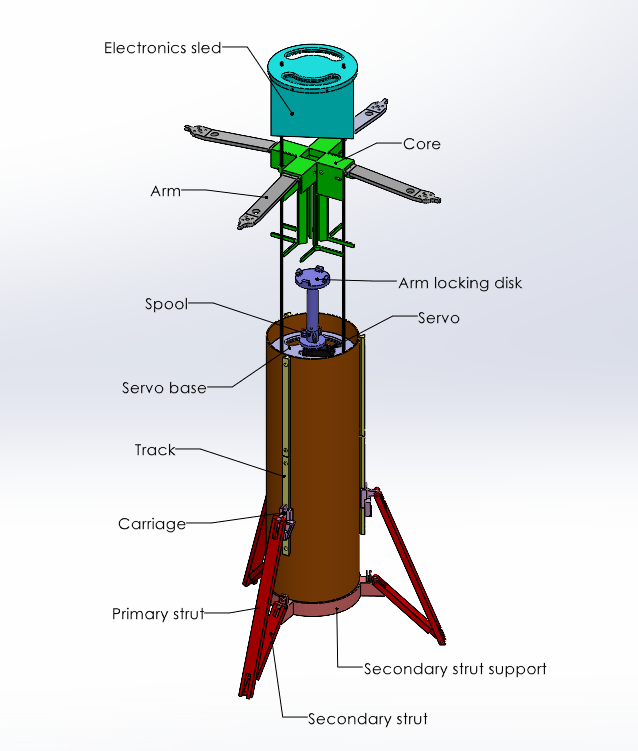
\includegraphics[width=\textwidth]{src/figs/full-labelled-cad-assembly.png}
    \caption{Full labelled CAD assembly without upper airframe}
    \label{arch:full-cad:labelled}
\end{figure}

\section{Control System Electronics Functionality}
The control system electronics are responsible for detecting whether the rocket is falling, deploying the propulsion arms and landing legs, and autonomous stabilization and navigation of the rocket. This system is composed of the Pixhawk flight controller which is responsible for running ArduPilot firmware for flight stabilization, a Raspberry Pi 4 model B flight computer which is used for running Python scripts for autonomous missions, an IMU for measuring acceleration, a radio transmitter for communicating with the QGroundControl groundstation application, electronic speed controllers for motor control, a 3S LiPo battery for the motors, and a separate rechargeable battery for the Raspberry Pi. A power distribution board is used to get power to all of the components. Images of the front and back of the avionics bay are shown in figures \ref{fig:AVF} and \ref{fig:AVB}.

\begin{figure}[H]
    \centering
    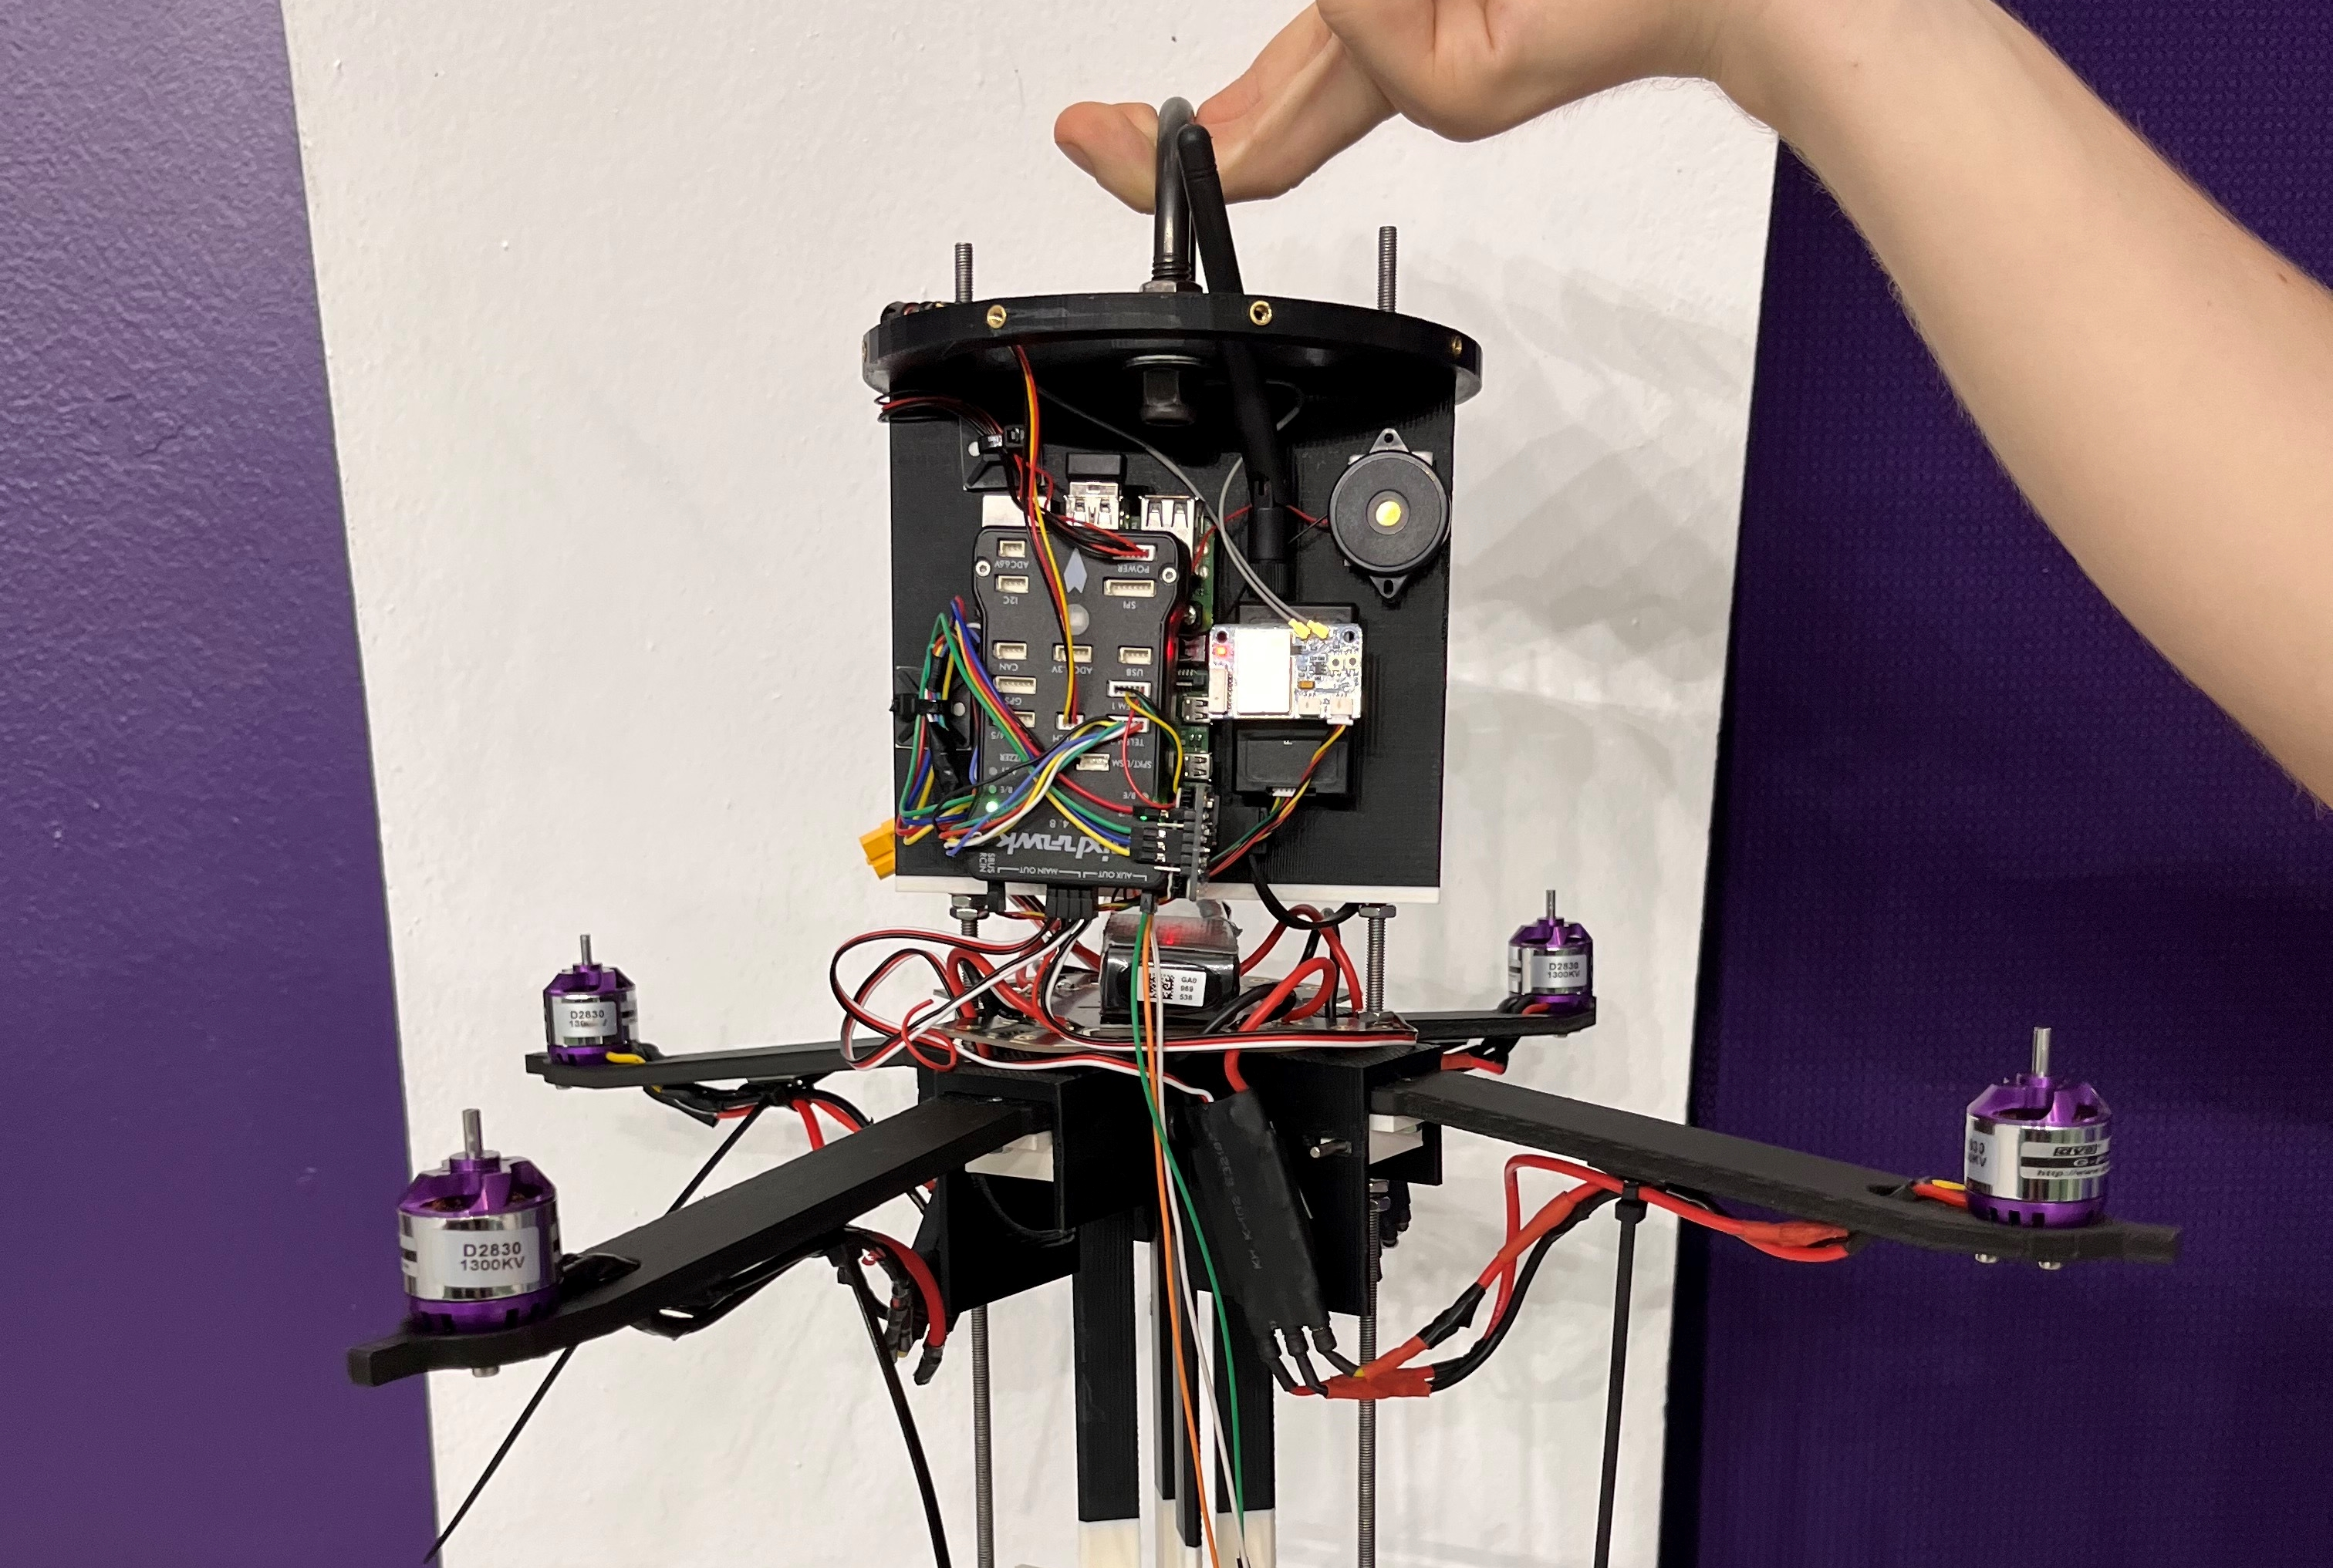
\includegraphics[width=\textwidth]{src/figs/AVBay_Front.jpg}
    \caption{Avionics Bay Front}
    \label{fig:AVF}
\end{figure}

\begin{figure}[H]
    \centering
    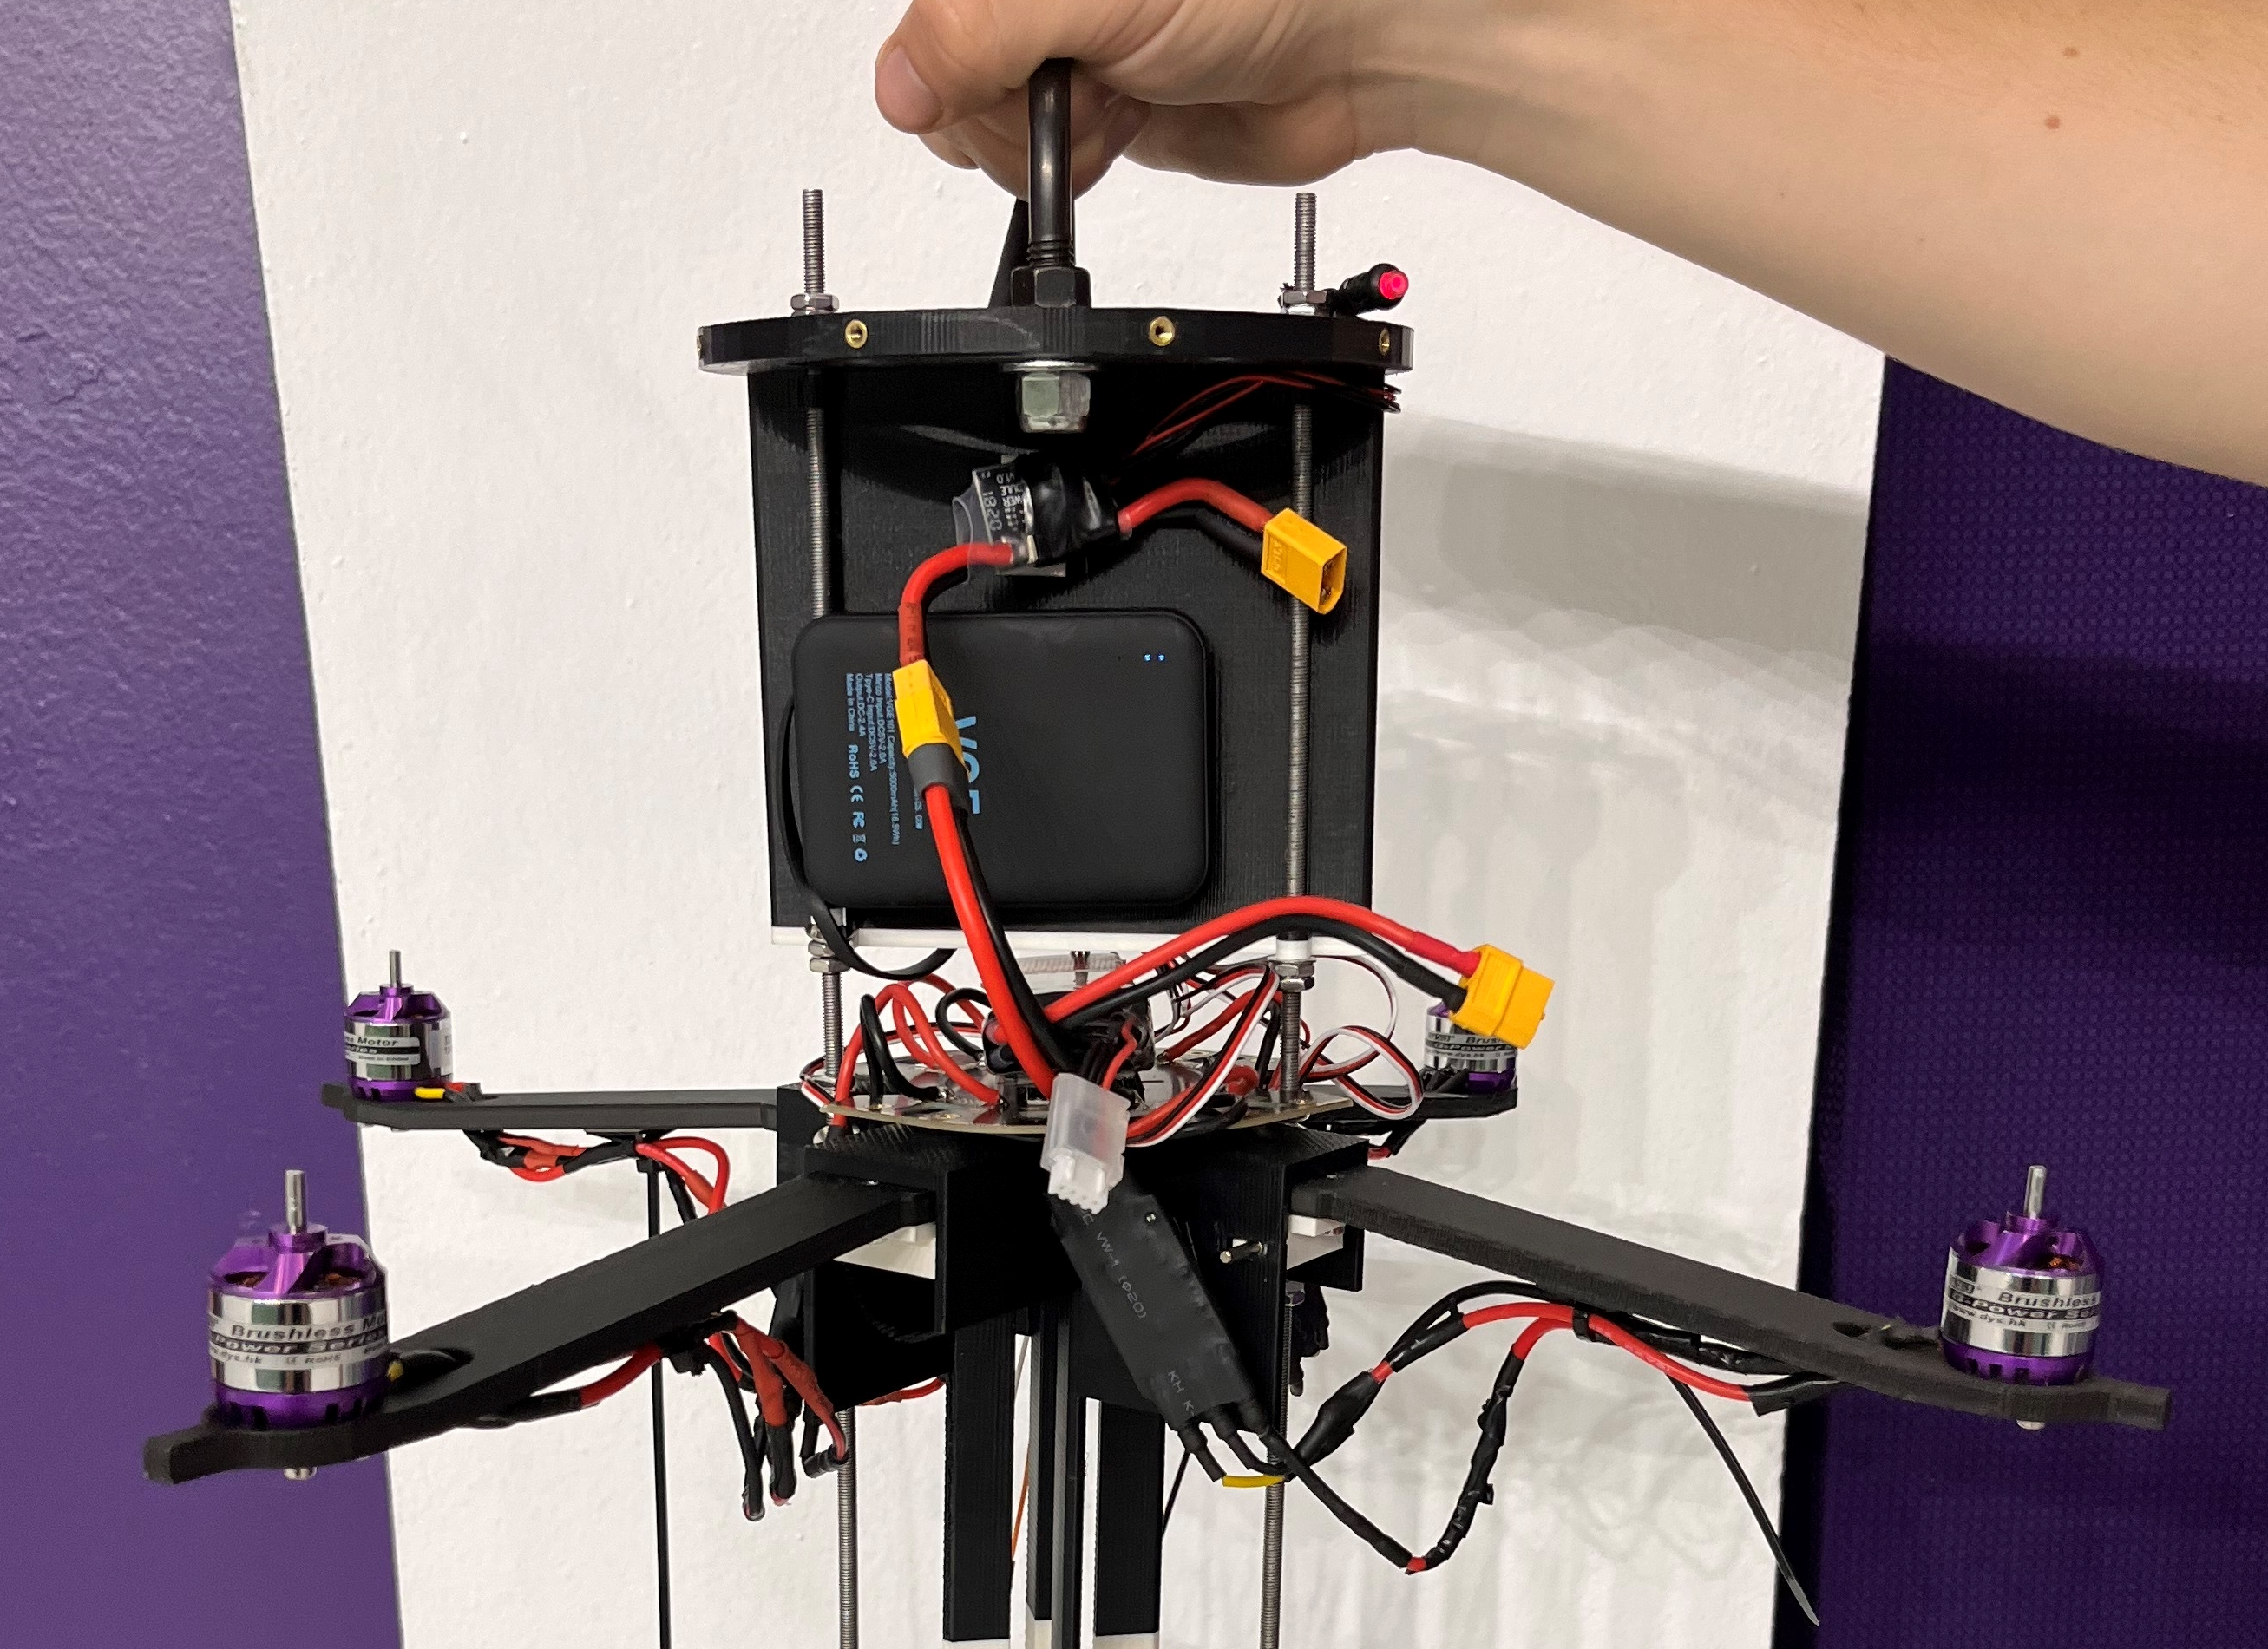
\includegraphics[width=\textwidth]{src/figs/AVBay_Back.jpg}
    \caption{Avionics Bay Back}
    \label{fig:AVB}
\end{figure}




\section{Propulsion Arm System Functionality}
The propulsion arm system is responsible for supporting the necessary components for lift generation as well as the components required to stow and deploy the system from the rocket body. The main component of this system is the propulsion arm which is solely responsible for providing a platform to which the motor mounts to and attaching to the rocket. The system is composed of 4 propulsion arms, each with an identical set of supporting components. The design of the arm was heavily driven by the development and design of these supporting components which are discussed below. The entire arm assembly will be explain and shown in figures in the following subsection.


\subsection{Upper and Lower Support Plates}
To simplify the assembly and maintenance procedures for the system, all components were designed to be modular and easy to remove from the rocket body. To facilitate this design requirement, two 10/32 aluminum threaded rods are vertically oriented on the inside of the rocket body. These rods are attached at their ends to two support plates which attach to the rocket body via 16 threaded inserts and accompanying M3 screws. The upper support plate has an extrusion below it that provides a flat mounting surface for a large portion of the control electronics. These are mounted above the propulsion arms in an effort to balance the moment caused by the landing legs to maintain the rockets center of mass as close to the center of thrust as possible.

\subsection{Deployment Method}
Each propulsion arm deploys through the use of two torsion springs which attach to the underside of the arm. When stowed, these springs are in their compressed position and actively trying to push the propulsion arms outside of the rocket body. Since the full travel from fully stowed to fully deployed for each of the arms is 90 degrees, torsion springs with a 120 degree free angle were selected to prevent over compression of the spring. To prevent premature deployment of the arms, a pre-deployment locking mechanism was developed that could simultaneously deploy all four arms on command.

\subsection{Pre-Deployment Locking Mechanism}
The pre-deployment locking mechanism is composed of a disk that rotates on command via a servo connected to it. The servo is recessed into the lower support plate via an interference fit cutout. It is then further secured to the plate via two bolts and nuts to prevent movement in the event of an unusual flight attitude. 

The disk has four protrusions or 'tabs' that are spaced every 90 degrees. These tabs interface with the arm when it is stowed in order to hold it inside the rocket body. Upon command, the disk rotates and the tabs are no longer aligned with the stowed arms allowing them to deploy to their operational position outside the rocket body. This all is shown in figure \ref{fig:stowedarm}.

\begin{figure}[H]
    \centering
    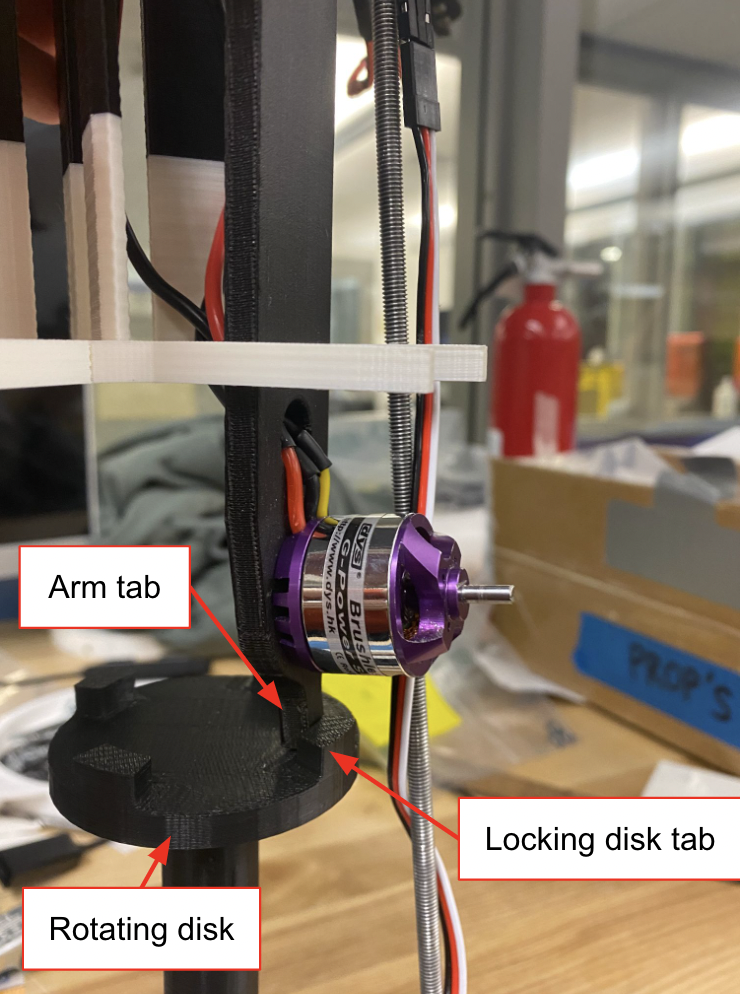
\includegraphics[width=0.6\textwidth]{src/figs/stowedarmlabeledview2.png}
    \caption{Stowed Arm in Locked Position}
    \label{fig:stowedarm}
\end{figure}

\subsection{Deployed Locking Mechanism}
Once the arms are outside of the rocket body, it is critical that they do not move around at all to prevent a moving center of thrust. To ensure that the propulsion arms remain in their fully deployed position, a deployed locking mechanism was developed. This mechanism involves a long-nose plunger spring pin which is mounted to the underside of the arm in a press-fit holder. The pin is compressed while inside the rocket but deploys into a small cutout when the arm has reached its deployed position to prevent it from falling below its fully deployed position. An image of this is shown in figure \ref{fig:deployedarm}.

\begin{figure}[H]
    \centering
    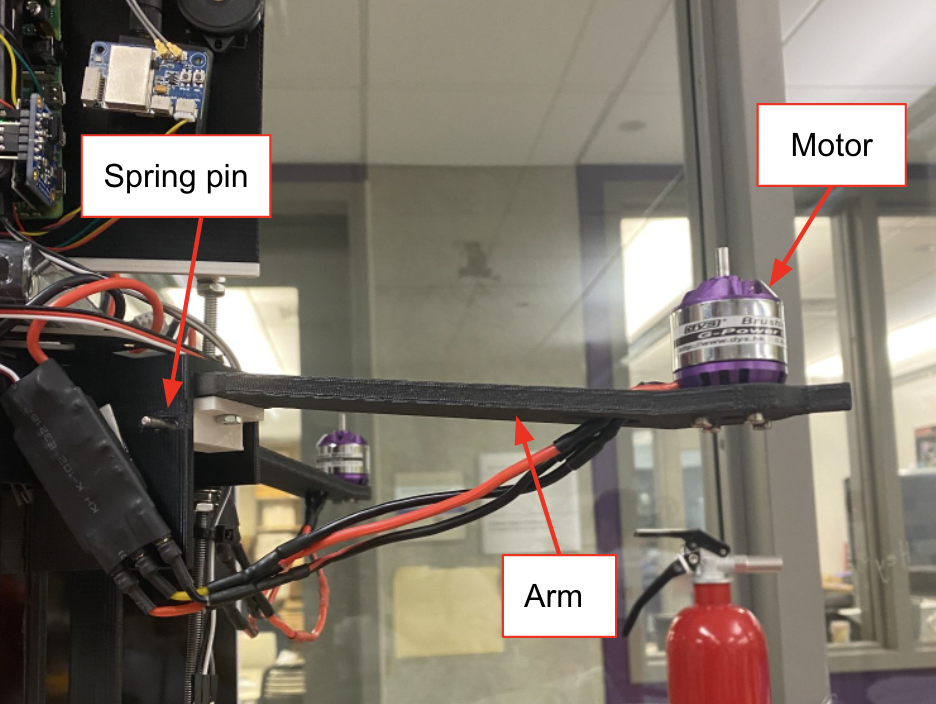
\includegraphics[width=0.9\textwidth]{src/figs/armdeployedlabeled.png}
    \caption{Deployed Arm with a Locking Mechanism}
    \label{fig:deployedarm}
\end{figure}

\subsection{Arm Core}
To facilitate the ability to remove all four arms at once for maintenance, they are all mounted to a centrally located 'arm core' as opposed to the actual rocket body. This component is mounted to the threaded rods via 8 nuts that are shouldered to prevent movement in the event of unusual flight attitude, vibration, and sudden acceleration. The arm core has four bays, one for each arm, that provide structures to support the deployment method, the propulsion arm, the deployed locking mechanism, the power distribution board (PDB), and the electronic speed controllers (ESCs).

Each arm is held in place by a 1/4" shoulder bolt that passes through both sides of the arm core bays, the arm, and the torsion springs. To support the torsion spring deployment method, each bay has a 30 degree slanted face that remains in contact with one end of the torsion springs. This face is slanted so that when the arm is fully deployed (a 90 degree offset from its stowed position), the 120 degree torsion spring is at its free angle. To help secure the torsion springs in their proper orientation, small tabs were added at the bottom of the slanted face to align the springs during assembly and prevent them from slipping out of place while compressed.

The top surface of the arm core is solid for two reasons. The primary reason for this design is to block the path of travel of the arm to prevent it from going beyond its fully deployed position and possibly having the propeller strike the rocket body. The secondary reason for this design is to provide a flat surface to which the PDB can mount.

Each bay also has two vertical walls on either side of the bay. These walls serve a variety of purposes. The primary purpose is to provide a surface to hold the deployed locking spring pin in its compressed position. The secondary purpose is to provide a flat mounting surface for the electronic speed controllers. One of these walls in each bay has a small cutout that allows the deployed locking spring pin to deploy into it when the arm reaches its fully deployed position, preventing the arm from moving below its deployed position. Extending below these main walls are two small structures that prevent the propeller from rotating inside the rocket body which could interfere with proper deployment.

\subsection{Propulsion Arm}
The propulsion arm is the primary component for this system but its design revolved heavily around the setup of the locking mechanisms and motor selection. 

At the end of the arm that attaches to the internal arm core, two protrusions are present that allow for the 1/4" shoulder bolt to pass through in order to securely attach to the arm core. Also, on this end of the arm are two small cutouts that extend 1.75" down the length of the arm. These cutouts provide a place for the torsion spring legs for deployment to slide into. This design ensures that the springs maintain their proper alignment while they are stowed. Finally, this end of the arm is also where the deployed locking spring pin attaches. This pin is connected via a press fit holder that is secured to the underside of the arm using counter-sunk through bolts. This pin holder also helps mechanically secure the springs to the arm, preventing them from disconnecting with the underside of the arm.

On the other end of the arm, 5 holes are included that provide mounts for the motor. Additionally, a small tab is present at the extreme of the arm. This tab is what interfaces with the pre-deployment locking mechanism to prevent the arm from inadvertently deploying before the landing system is called to action.

In order to accommodate the large motors required for the thrust needed, the arm has a 5/8" dip in it from the point it exits the rocket body to the point that the motor attaches. This dip was necessary to ensure that all components when stowed fit inside the confines of a 6" rocket body. 

\section{Landing Leg System Functionality} 
The landing legs support the rocket body upon landing and ensure that the rocket body lands upright in a stable position. The main components of this system are the primary and secondary strut which together distribute the loading upon landing impact, one locking mechanism to lock the leg in its stowed position, another single locking mechanism to lock the leg in the deployed position, and a deployment mechanism that provides the force to deploy the leg. This system is composed of 3 landing legs each spaced at 120 degrees from each other. Each landing leg is composed of the primary strut, secondary strut and supporting components, all of which are discussed below. All components with the exception of one are mounted to the outside of the rocket body using M3 bolts. To provide a flat mounting surface for the nut on the inside of the rocket, small internal mounts were printed that match the inner diameter of the tube on one side and are flat on the other. The bolt for each component passes through the component, the rocket body, then this part.

\subsection{Primary and Secondary Struts}
The landing leg uses a 2 strut system in which a primary and secondary strut are attached at the point that will contact the ground upon full deployment. When stowed both components run vertically up the side of the body tube. An image of the leg in the stowed position is shown in figure \ref{fig:LegStowed}. When deployed, they form a triangle that contacts the rocket in two places and the ground in one. The ends of the legs that attach to the rocket are also hinged using shoulder bolts to allow them to easily move to their deployed position when unlocked. The secondary strut is hinged in a fixed location at the very bottom end of the rocket body. In order to allow for the struts to move between their compact, stowed position along the sides of the rocket to their deployed position, a track and carriage system is needed. The primary strut is hinged to the carriage which has the ability to move up and down along the track mounted to the side of the rocket. The design of the track and carriage relied on the deployment method and locking mechanisms discussed below.

\begin{figure}[H]
    \centering
    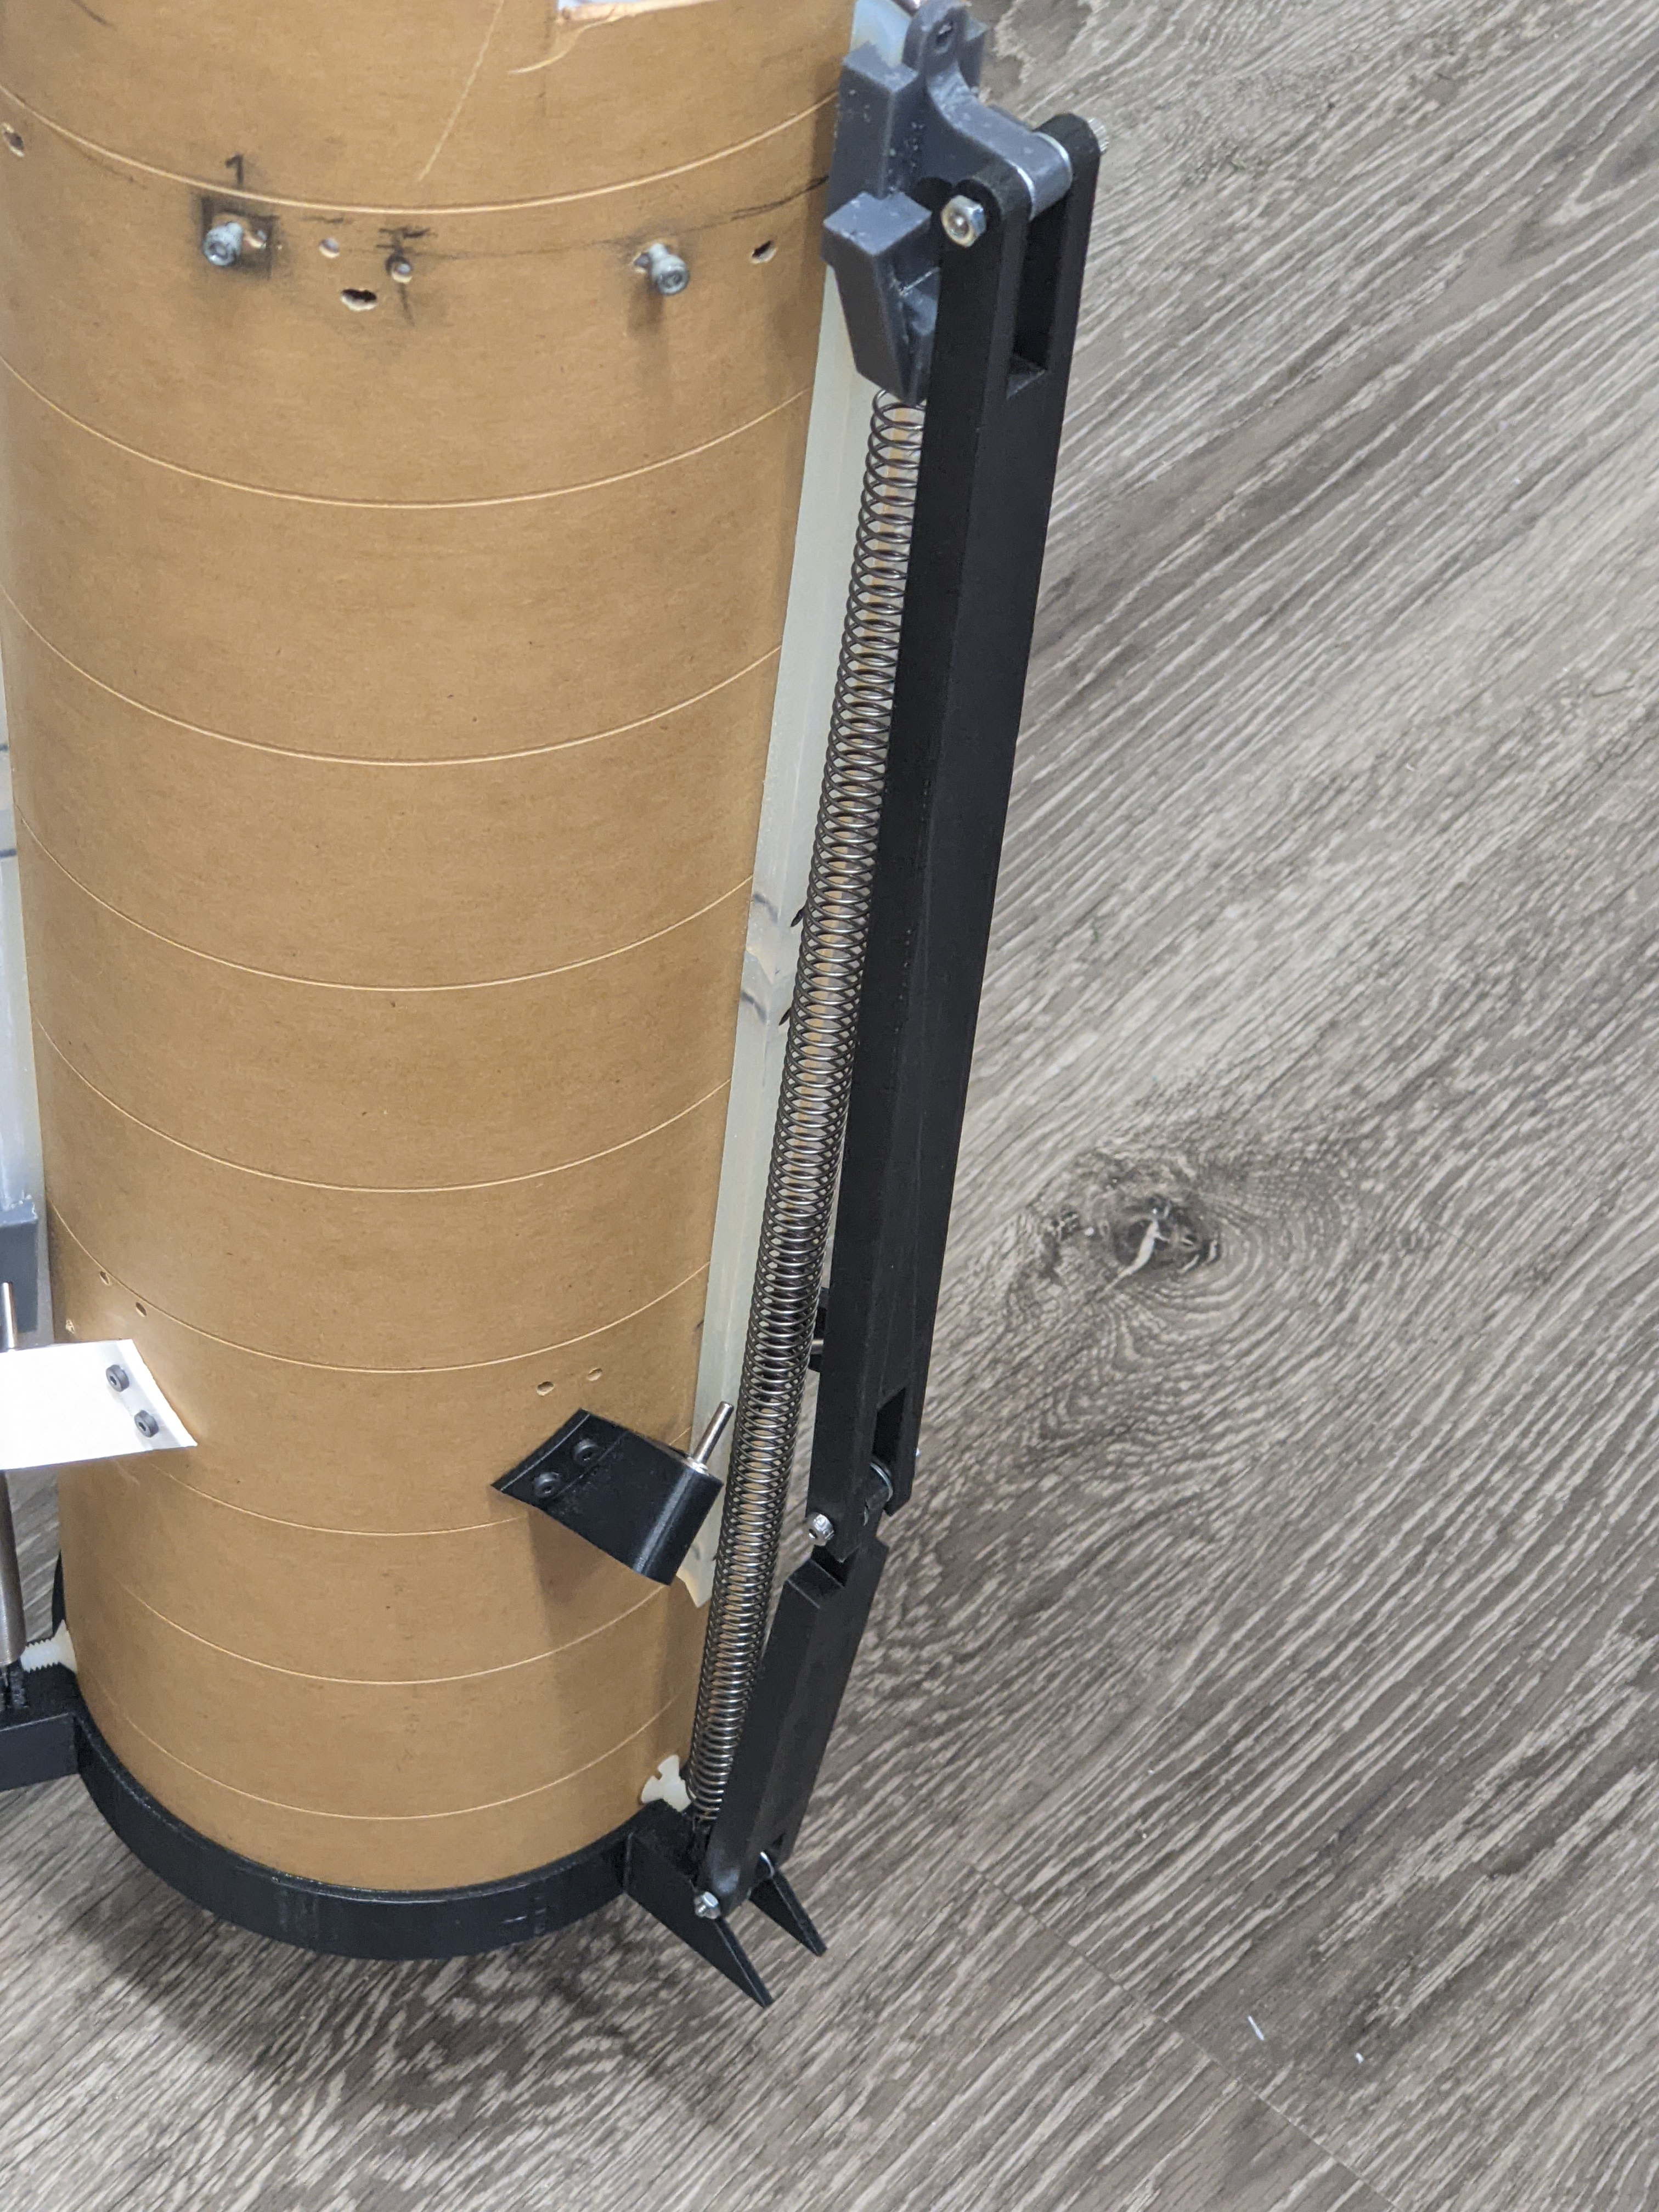
\includegraphics[width=0.5\textwidth]{src/figs/Stowed_Leg.jpg}
    \caption{Leg in Stowed Position}
    \label{fig:LegStowed}
\end{figure}

\subsection{Deployment Method}
Since the deployment relies on a track and carriage system, a linear spring was selected as the leg deployment mechanism. The spring attaches to the primary strut carriage at one end and a mount at the bottom of the rocket body at the other end. When fully stowed, the spring is pulling down on the carriage to bring it to its deployed position. Once fully deployed, the spring is still in a small amount of tension in order to keep force pulling the leg down and provide a small amount of suspension upon impact with the ground.

\subsection{Pre-Deployment Locking Mechanism}
To hold the leg in the stowed position, a pre-deployment locking mechanism is installed that restrains the motion of the carriage into its stowed position. This mechanism relies on the same servo as the propulsion arm pre-deployment locking mechanism. The mechanism consists of a 'spool' with three attach points. The spool is secured to the servo using a 50mm M3 bolt as well as cutout on its underside to prevent the spool from slipping (figure \ref{fig:spoolc}). The propulsion arm 'disk' is attached to this spool by sliding over it and then being secured with M2 screws in threaded inserts. Attached to the spool at the 3 attach points are pins pass through the rocket body and into the back of the carriage. When the spool is rotated, these pins are pulled out of the back of the carriage, allowing it to be pulled into the deployed position by the attached linear spring. 

\begin{figure}[H]
    \centering
    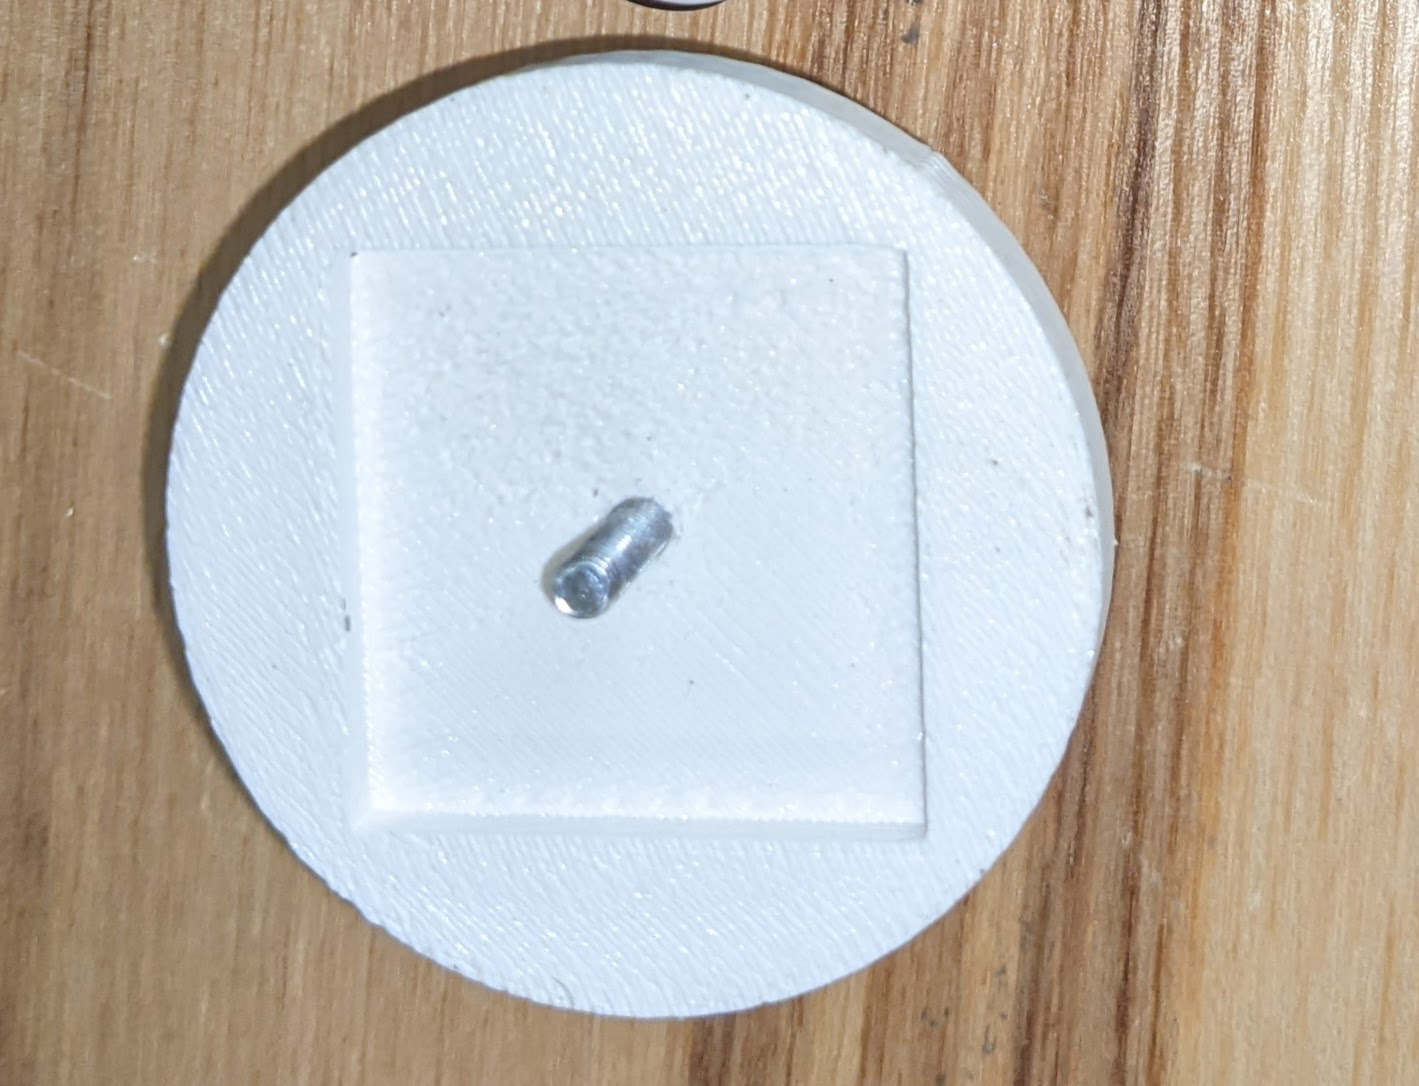
\includegraphics[width=0.5\textwidth]{src/figs/Spool_Cutout.jpg}
    \caption{Cutout Underneath Spool}
    \label{fig:spoolc}
\end{figure}

\subsection{Deployed Locking Mechanism}
Once fully deployed, a pair of spring pins holds each landing leg in its fully deployed position. Both pins are mounted just above the carriages fully deployed position facing slightly upwards. As the carriage is pulled past them, they compress, allowing the carriage to pass. Once the carriage has passed the pins, they return to their extended position which blocks the carriage from being able to slide back up the track when weight is placed on the landing legs. An image of the pin inside the core is shown in figure \ref{fig:pin_rocket}.

\begin{figure}[H]
    \centering
    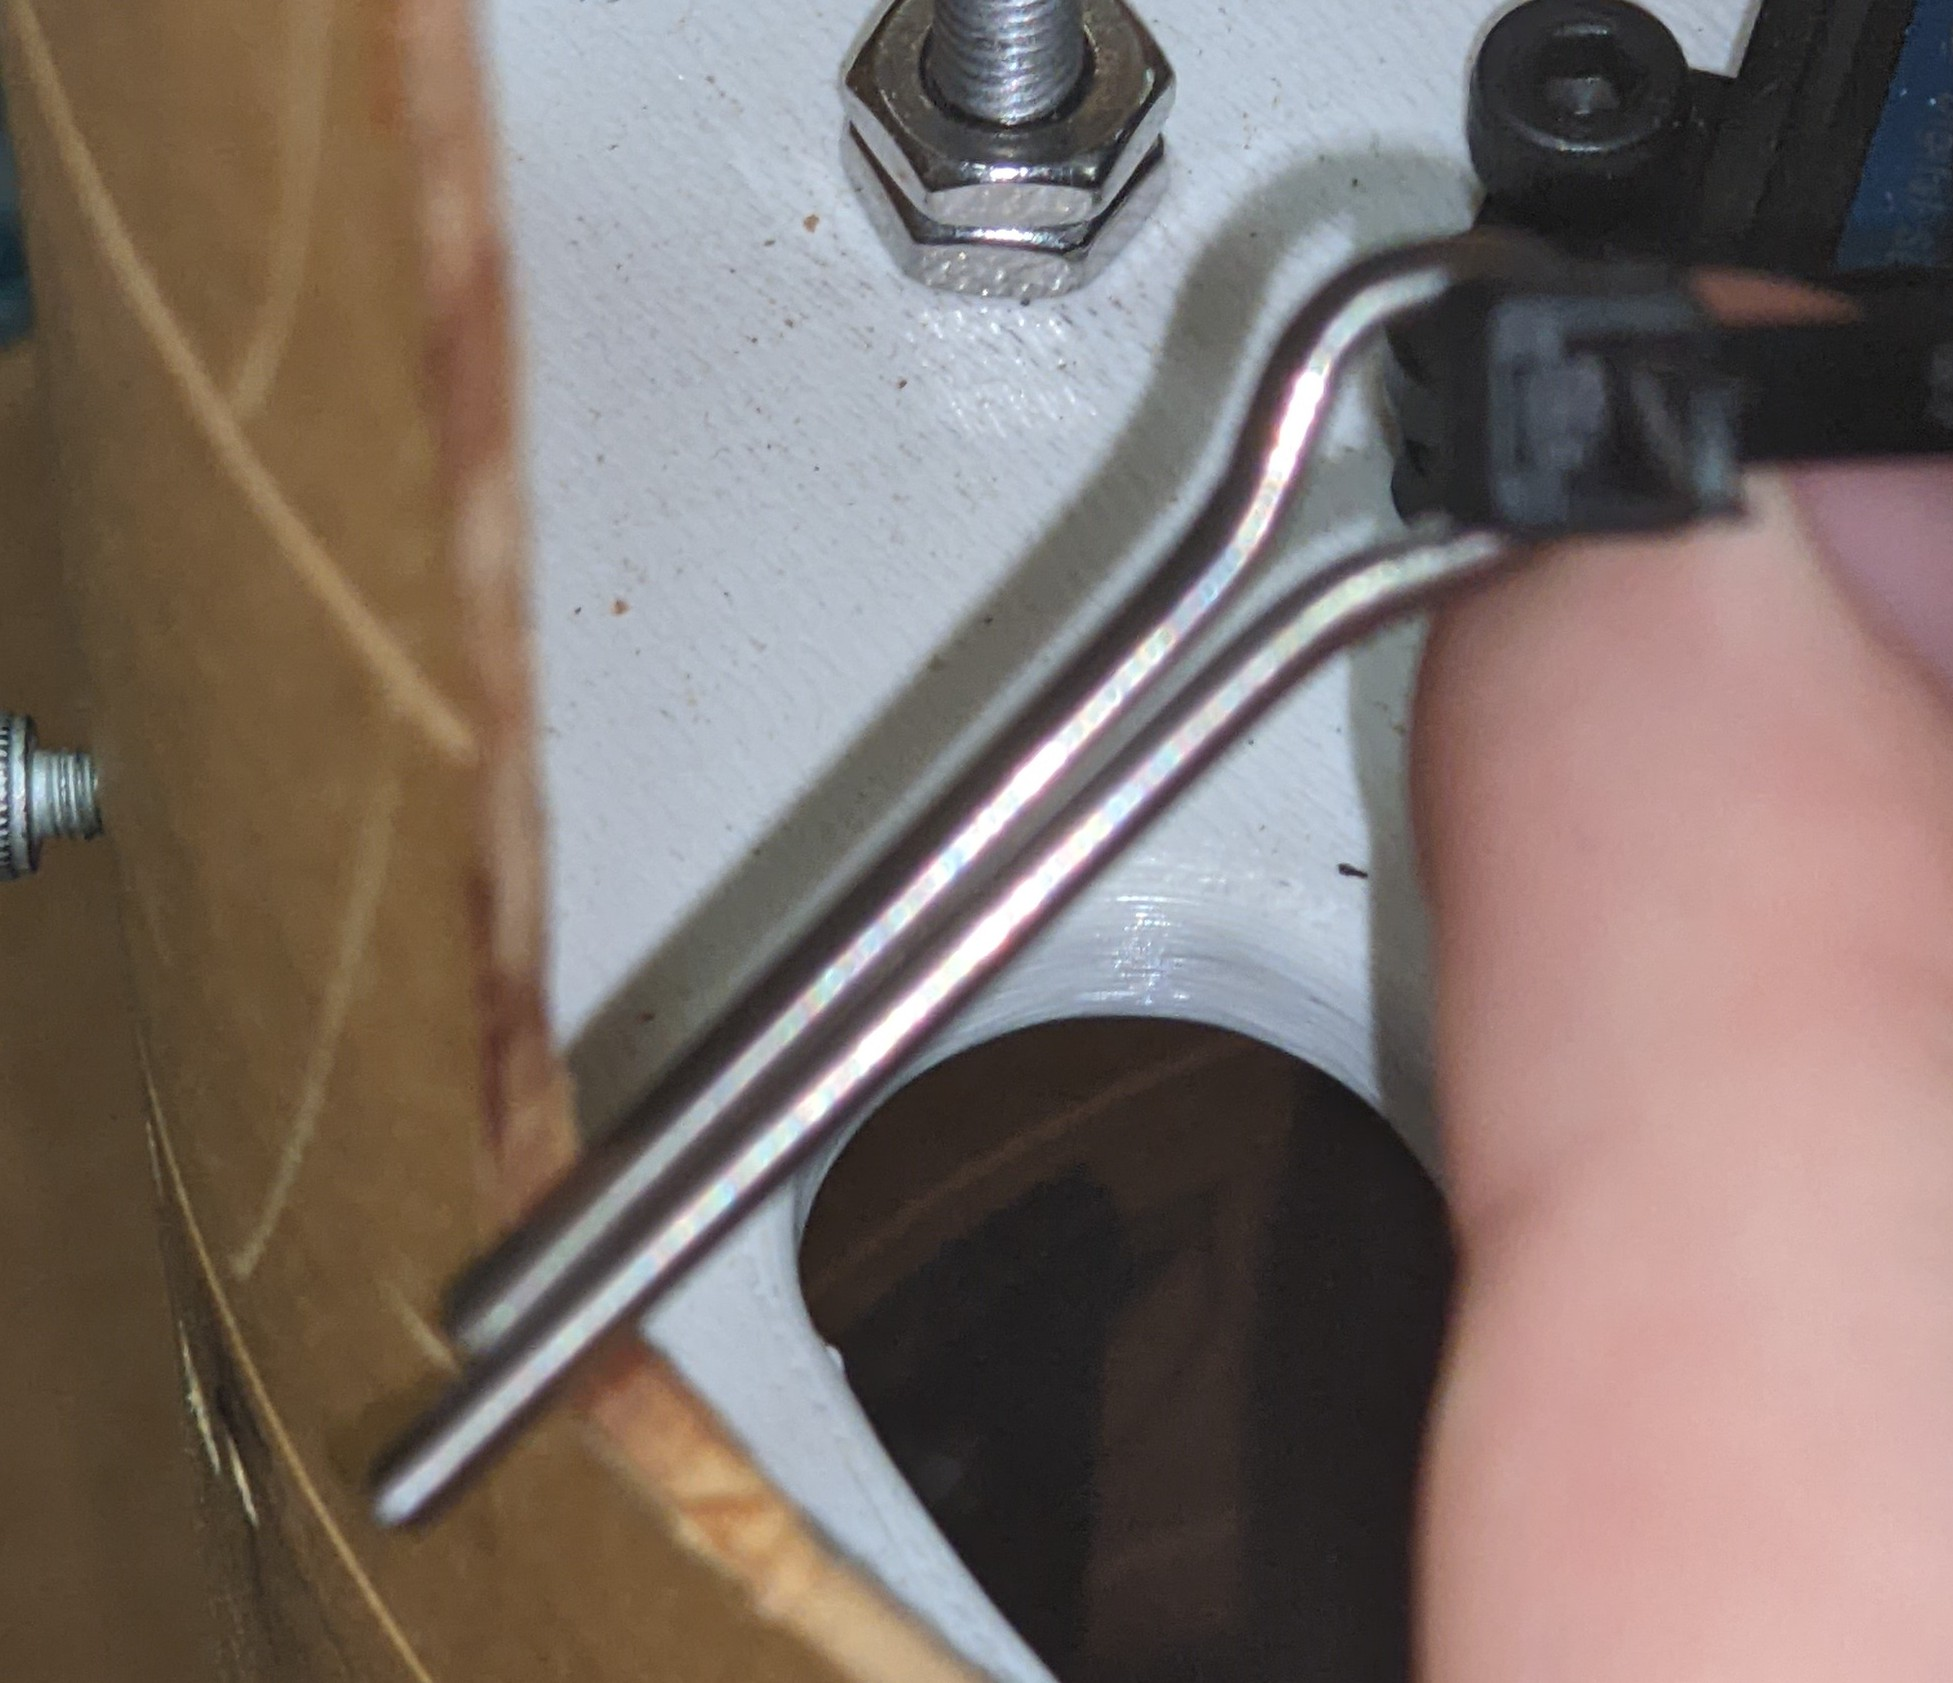
\includegraphics[width=0.5\textwidth]{src/figs/Pins_Rocket.jpg}
    \caption{Pins to Stow Rocket}
    \label{fig:pin_rocket}
\end{figure}

\subsection{Track and Carriage}
The track and carriage are designed to function without the use of any form of bearing or lubrication. They use a nested design in which the track mounts to the rocket body and the carriage is shaped so that it is constrained to only motion in the direction necessary with small clearance for very minor side to side movement (figure \ref{fig:CLB}). 

\begin{figure}[H]
    \centering
    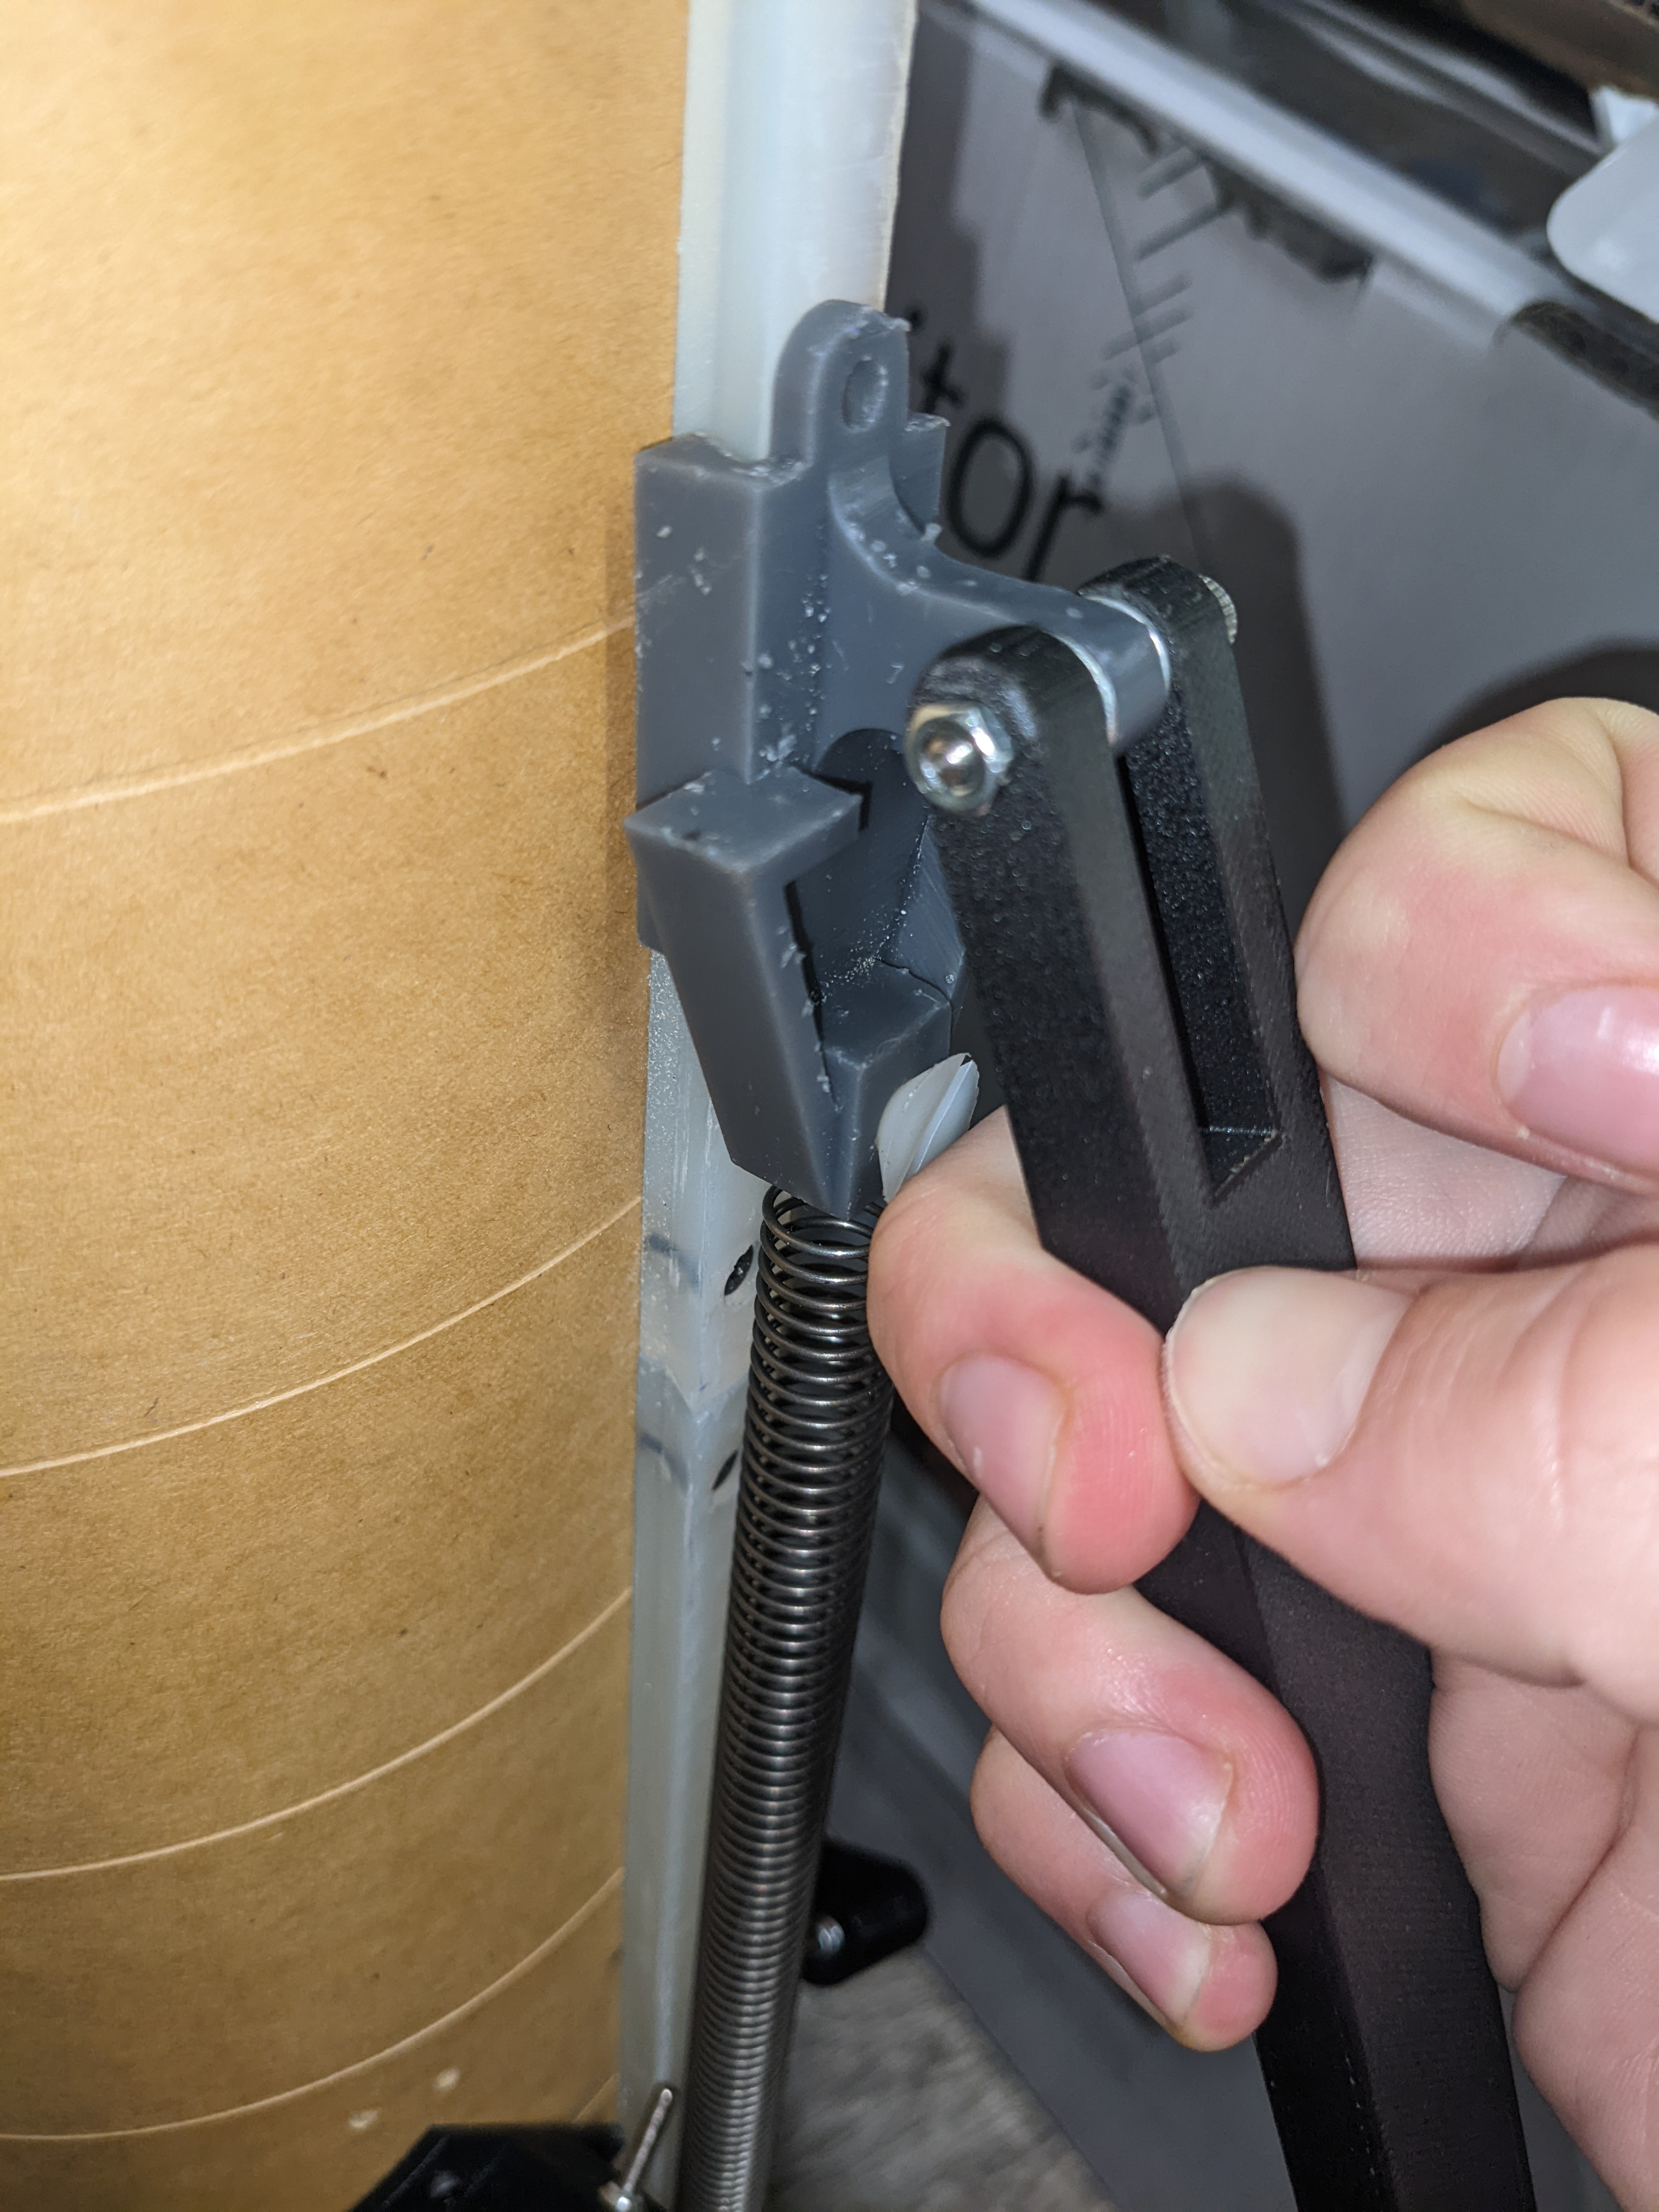
\includegraphics[width=0.35\textwidth]{src/figs/Carriage_Leg.jpg}
    \caption{Carriage on Leg Bracket}
    \label{fig:CLB}
\end{figure}

The carriage has an attach point for the primary strut that protrudes from the carriage surface. Additionally, a mount point for the upper end of the spring is present. The spring goes into the slot in the carriage and is secured by a plastic screw that passes through the carriage and center of the spring hook. A small protrusion and hole is added to the very top of the carriage through which the pin for the pre-deployment locking mechanism passes. On the sides of the carriage, angled walls are present to push the deployed locking pins into their housing while the carriage passes. Just beyond these angled walls, the carriage narrows, providing a contact surface for the deployed locking pins and the carriage.

\subsection{Secondary Strut Support}
To prevent the landing leg system from traveling beyond its ideal deployed angle of 40 degrees (see Section \ref{ea:landing-legs}), a lower support is in place that stops the secondary strut from travelling beyond 135 degrees from its stowed position. This support is one ring that contains an angled surface for each leg set. The ring not only helps with alignment since all three leg supports are mounted together, but also distributing the load of impact around a larger area of the body tube to minimize the risk of component failure. On each of the support faces is a hinge point for the secondary strut as well as an attachment point for the lower end of the deployment spring. The spring here is also held in place through the use of a through screw that is constrained from coming out by the screw head as well as the rocket body.
\chapter{Design Approach and Solutions}
\label{design-approach}
Due to the complexity of the system and highly interconnected setup of components, the design process throughout both quarters was a fast-paced, highly iterative design process that saw hundreds of models produced and dozens tested. The following sections detail the initial design and development of each component on the alpha prototype.

\section{Initial Research, Testing and Prototype Development}
Prior to dividing the prototype into 3 distinct, but communicating systems, research was conducted for various options for propulsion and deployment mechanisms. 

\subsection{Propulsion Selection}
Most traditional rocket landing systems use a gimballed thrust vector control system together with a combustion based engine to land the rocket (see Section \ref{competitive-analysis}). However, one of our client's requirements was that combustion not be used to land the rocket. This also ties in with the needs and specifications outlined in Section \ref{needs-and-specs}, specifically need \#10 which states that the product must follow competition guidelines, and one of the guidelines specifically prohibits the use of explosive materials during landing. With this requirement in mind, the team set out researching a variety of different propulsion methods ranging from water jets to ducted fans. 

One of the solutions that was analyzed was the concept of cold gas thrust. Cold gas thrust is already commonplace in the aerospace industry and it would potentially allow us to use existing infrastructure. Despite its potential, cold gas is almost exclusively used for minor trajectory corrections or slowly propelling astronauts on space walks, never for outright propulsion. To determine whether or not cold gas thrust could work for our client's purposes, an computational fluid dynamics simulation using ANSYS Fluent was conducted to determine the feasibility of this solution. It was found that using this form of propulsion would require the addition of up to 15kg of compressed gas, tanks, and regulators the system, rendering it completely unfeasible. For more information on this simulation, please see Appendix \ref{app:cold-gas-thruster}.

After this calculation was completed, the team was able to narrow in on the propulsion front runners through the use of an alternatives matrix (figure \ref{fig:PAM}). After more in depth research on minimum sizes and maximum thrusts of the front runners, the team proceeded with a quadcopter style propulsion system in which four motors would be mounted in a square pattern and would be controlled by an onboard avionics suite. 

\begin{figure}[H]
    \centering
    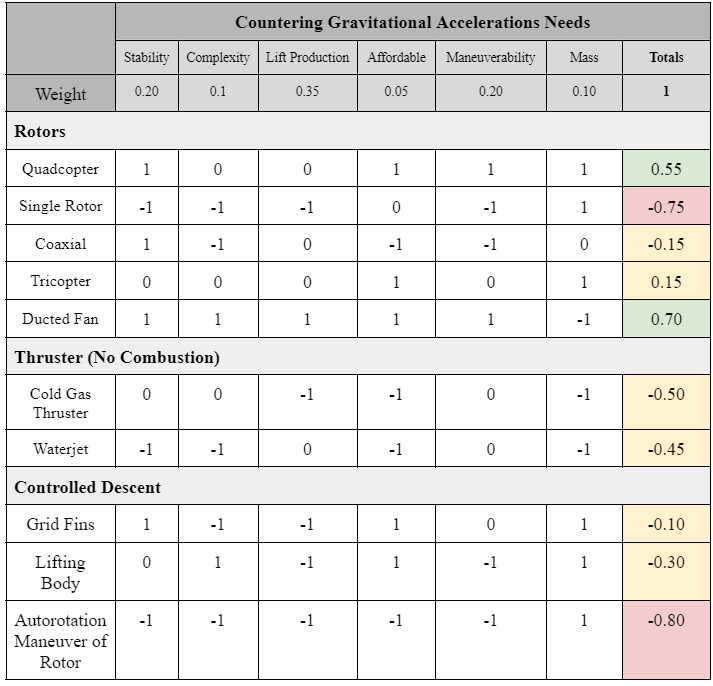
\includegraphics[width=0.5\textwidth]{src/figs/AltProp.png}
    \caption{Propulsion Alternative Matrix}
    \label{fig:PAM}
\end{figure}

\subsection{Deployment Research and Development}
Deciding to go with a propeller based system provided the team with a new challenge to navigate; these four propellers now had to be able to be stowed inside a cylinder that is a smaller diameter than they are. In order to accomplish this, the arms would need to be fixed at some point in the body and swing out to their deployed position. Design focus quickly shifted to developing this system so it could be tested and iterated. The initial idea was the use of 4 servos, one on each arm that would actuate the arm 90 degrees to its deployed position. This method was tested using a light servo that was believed to have enough torque to deploy the arm. However, it was quickly found that the servo purchased could not move the arm as fast as we needed it to and increasing the torque of the servo was not an option because of size and mass constraints. 

The team began looking into deployment methods that could use one centralized servo to deploy all four arms simultaneously. Initial ideas involved the use of a complex gear system to take rotation from the servo and change its rotation direction to deploy the arm 90 degrees. This idea was quickly written off due to its mechanical complexity. The other leading deployment option was through the use of torsion springs. Torsion springs provided a lightweight, reliable and fast solution to deploy the arms from inside the rocket body. 

In order for torsion springs to work, a mechanism to keep the arms inside the rocket also had to be developed. With the teams goal of finding a solution that allowed the use of one actuator to control four components, the idea of a centrally located unlocking disk emerged. This disk would have 4 protrusions that blocked the arms from deploying from the rocket. When thrust was needed, the disk would rotate via a single servo. This would move the protrusions from the arms path of travel, allowing the torsion springs to push them to their deployed position.

Once the unlocking system had been designed, an accompanying arm was designed that had a small rectangular protrusion on the motor end that would interface with the unlocking disk while the arm was stowed. 

These components were all printed or purchased and combined to form the teams critical system prototype the Arm Deployment Test Stand (ADTS). The image of the original ADTS is shown in figure \ref{fig:ADTS}. The following sections detail the design process since the quarter 1 critical system prototype delving into changes made to the ADTS system as well as the component creation and iteration.

\section{Motors and Blade Selection}
\label{design:motors-selection}
Once the team had decided on using propellers for the propulsion mechanism, the next step was to select the appropriate motor and blade to generate the thrust required to slow down and maneuver the rocket while it's falling. For this the team made heavy use of the Static Thrust Stand (STS) that was constructed during Quarter 1. Although a simulation driven approach to motor and propeller selection could have been attempted using various computational fluid dynamics packages such as ANSYS Fluent, it was determined that a quicker and more accurate approach would be to obtain empirical data for thrust generated by different motor and blade combinations using the STS. The static thrust stand, pictured in Figure \ref{design:STS}, features a load cell, load cell amplifier, Raspberry Pi computer, and electronic speed controller (ESC) which work together to log thrust values produced by the motor/propeller that is mounted to the load cell. The data is then saved and plotted which serves as an excellent way to determine what the ideal motor and blade combination will be. Furthermore, the Python code used for the STS can be found in Appendix \ref{app:sts-code}.

\begin{figure}[H]
    \centering
    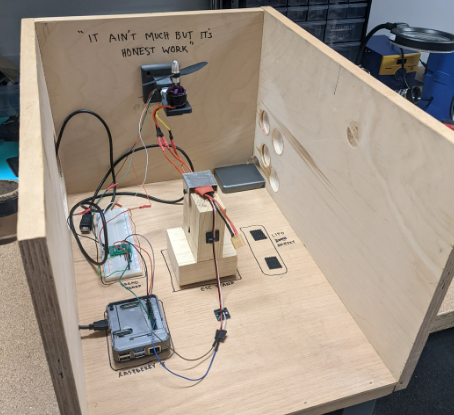
\includegraphics[width=0.75\textwidth]{src/figs/STS.png}
    \caption{Static Thrust Stand (STS)}
    \label{design:STS}
\end{figure}
Figure \ref{design:diff_blades} shows the thrust produced by several different blade sizes with the same motor. The team determined early on that the primary factor that affects thrust is the blade diameter, while pitch and blade shape have a less significant effect.
\begin{figure}[H]
    \centering
    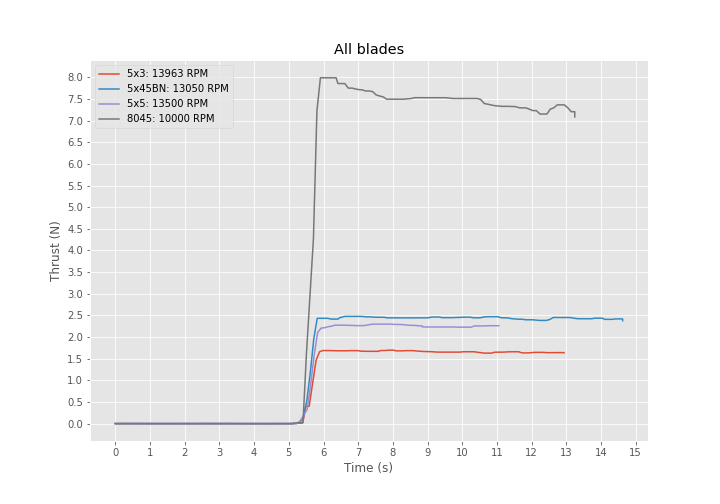
\includegraphics[width=0.85\textwidth]{src/figs/STS_4_diff_blades.png}
    \caption{Comparison of thrust for different blades}
    \label{design:diff_blades}
\end{figure}

Initial mass estimates of the final fully assembled rocket dictated the amount of the thrust that would be needed to stop and land the rocket. Further calculations to determine an acceptable thrust to weight ratio were conducted as well and can be found in Section \ref{thrust_analysis}. At this stage, the team began by testing several different motors and blades. First, in an effort to achieve the highest possible RPM, several high kv (RPM/volt), low stator size motors were tested to see if they would give ample thrust. Plots from the static thrust can be seen in Figures \ref{design:sts:2450} and \ref{design:sts:2550}. Unfortunately, these motors were not a good choice since the low stator size equates to lower torque capabilities. This is evident from the plots of thrust versus time since the thrust continually decayed as time went on. Additionally, over-torquing the motors resulting in lots of excess heat being generated outside of nominal operating temperatures.
\begin{figure}[H]
    \centering
    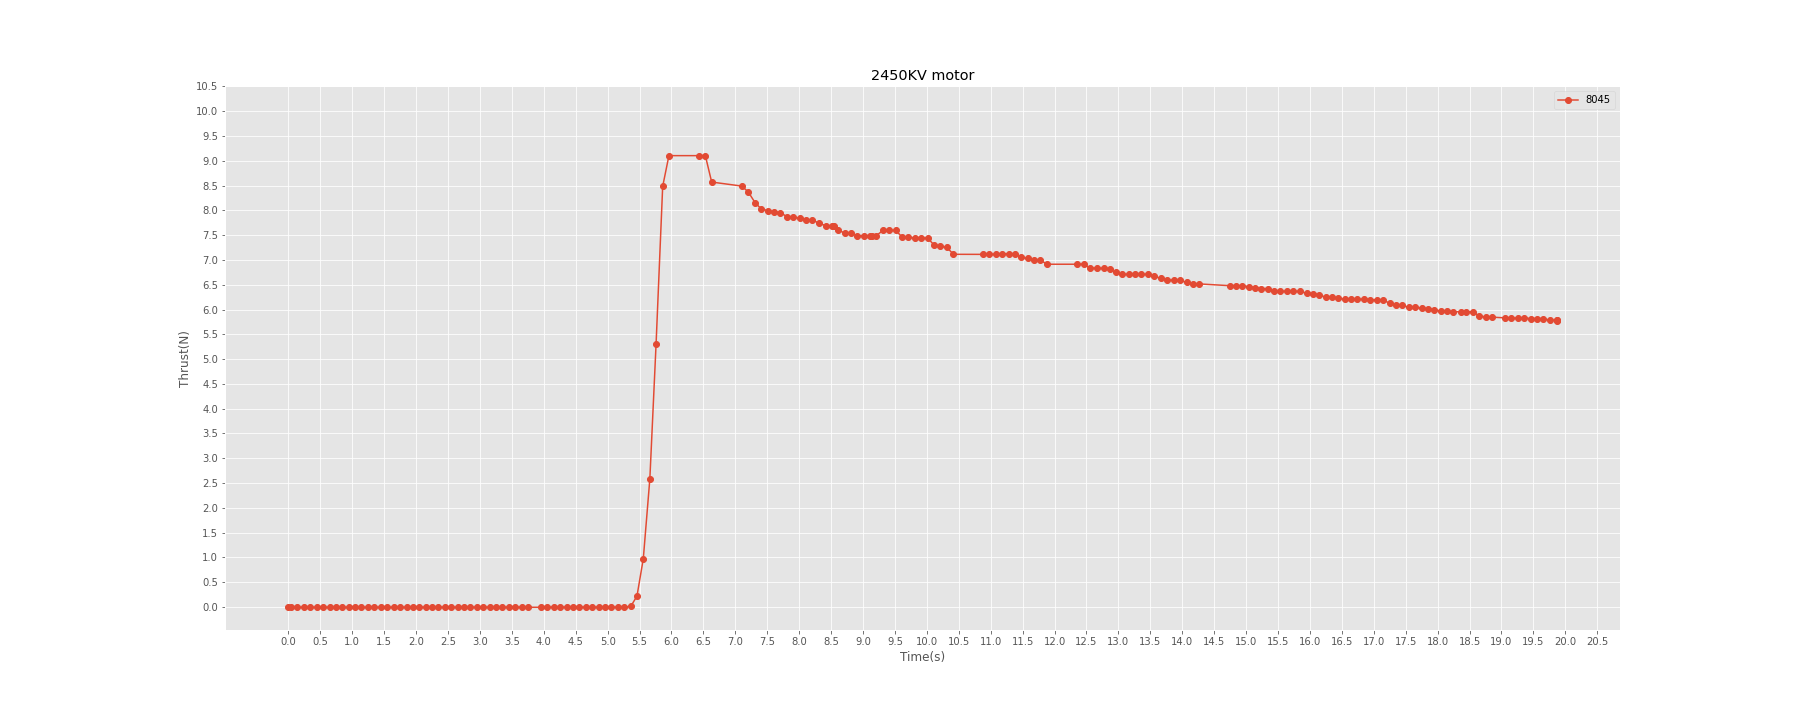
\includegraphics[width=\textwidth]{src/figs/small_2450_motor.png}
    \caption{2450 KV motor}
    \label{design:sts:2450}
\end{figure}

\begin{figure}[H]
    \centering
    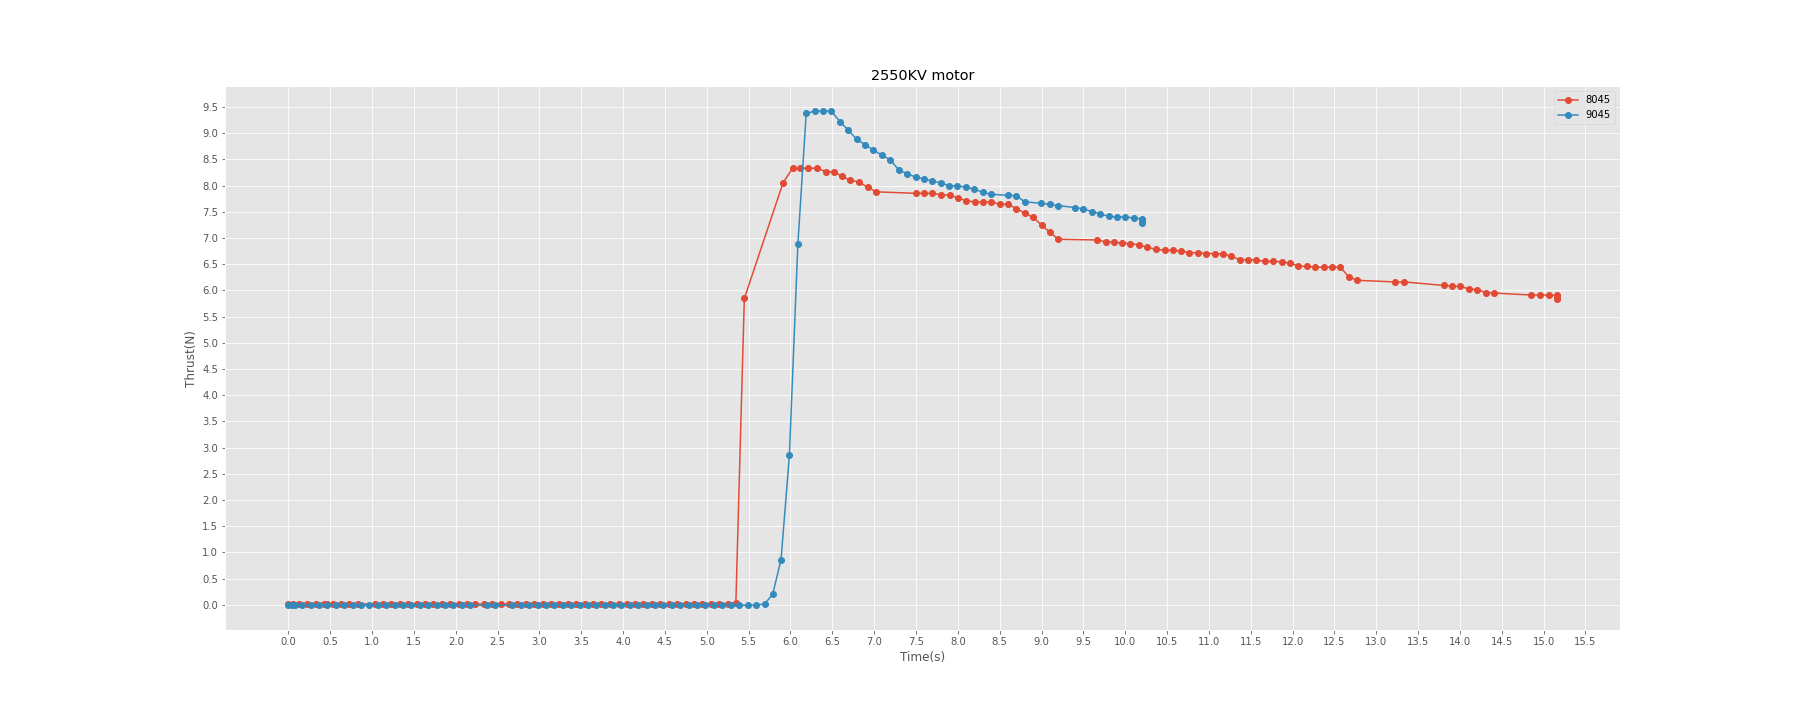
\includegraphics[width=\textwidth]{src/figs/small_2550_motor.png}
    \caption{2550 KV motor}
    \label{design:sts:2550}
\end{figure}
Once it was determined that higher torque motors were needed, the team tested some larger stator size motors with several different blades and were very pleased with the results. The larger motors were capable of outputting the torque needed to spin the blades at speed while also producing substantial thrust. The thrust versus time plot for this new motor is shown in Figure \ref{design:sts:purple}.
\begin{figure}[H]
    \centering
    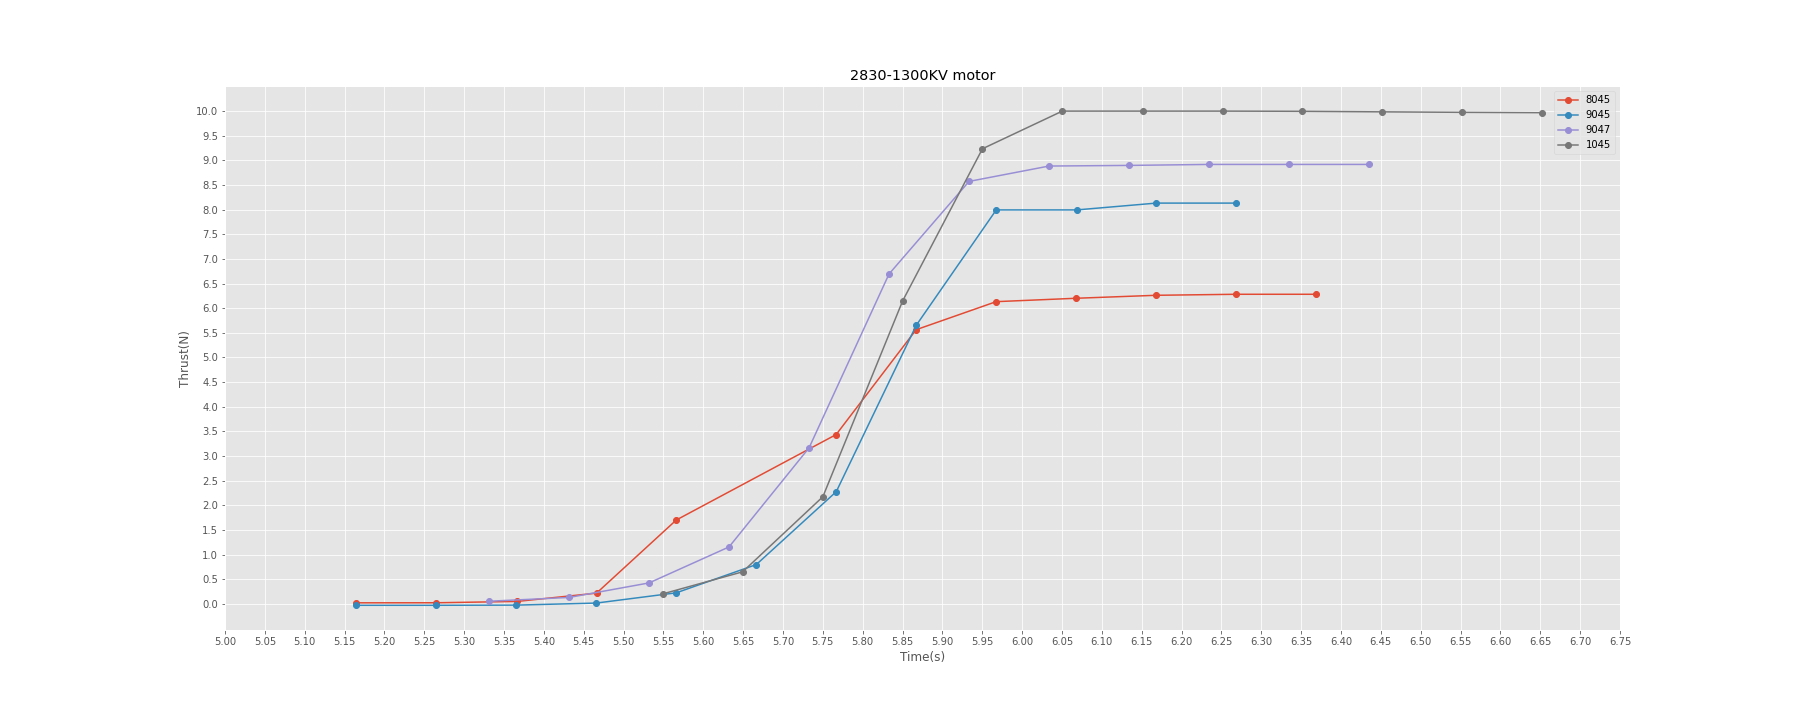
\includegraphics[width=\textwidth]{src/figs/purple_motor.png}
    \caption{1300 KV motor}
    \label{design:sts:purple}
\end{figure}
At this stage through the thrust to weight ratio analysis presented in Section \ref{thrust_analysis}, and with the current mass estimate of between 3 and 4kg, the team decided that the best choice would be to find a motor that could produce even more thrust than the  1300 KV motor in Figure \ref{design:sts:purple}. Eventually, the team found two different motors with very high torque and RPM capabilities, however they required a larger LiPo battery as well as a electronic speed controller (ESC) with a higher current rating. In the end, due to time constraints the team was not able to calibrate and test these new motors, however as will be made clear in later discussions, the setup of the electronics and software allows for motors to be "plug-and-play" and swapping out motors later on will require little to no modification to other aspects of the project. In conclusion, the team decided to move forward for now with the 1300 KV motors that were shown to produce around 10N of thrust on average.

To ensure this motor truly had to power needed, an endurance test was conducted in which the motor was throttled to 90\% for 60 seconds to determine if there was any thrust loss over time like there was with the lower torque motors. Figure \ref{design:sts:endurance} shows the results of this endurance test. Although there was some decay in thrust, the average thrust for the first 20 seconds was larger than 10N, which is presumably sufficient considering the expected mass of the rocket and flight time.
\begin{figure}[H]
    \centering
    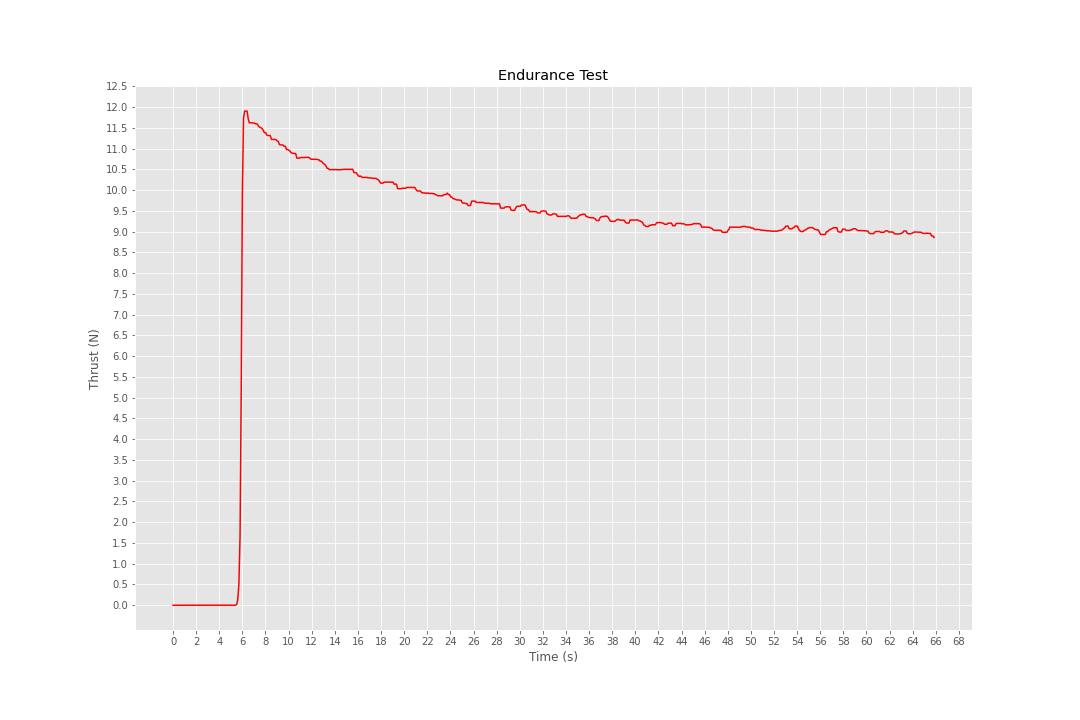
\includegraphics[width=\textwidth]{src/figs/purple_endurance.png}
    \caption{1300 KV motor endurance test}
    \label{design:sts:endurance}
\end{figure}


\section{Control System Electronics}
The onboard software and electronics are designed to detect when the rocket is falling, deploy arms and landing legs, and spin motors to enable a controlled descent and landing of the rocket autonomously without human intervention. Early on in the design and development stage of the project, the team realized that once the arms have been deployed, from an electronics and software perspective, the problem at hand is being able to autonomously "catch" and land a falling quadcopter. We operated on the assumption that the rocket being attached will make little to no difference so long as additional weight and an adjusted center of mass are accounted for. This being said, the team began by testing all electronics and software with a custom built quadcopter in parallel with the design of the rocket's arm and landing leg deployment mechanisms. This afforded the team the ability to develop each subsystem independently, and assemble components later on in a modular fashion.

\subsection{Hardware}
\label{design:controls:hardware}

\paragraph{Motors}

The voltage and current draw of the motors dictate the requirements of all other controls hardware. Quadcopters most commonly use three channel brushless DC motors due to their robustness and variety.

Brushless DC motors have fixed array of magnets on the inside of their rotor. The rotor interfaces with a stator composed of a complimentary array of wound copper wires. When a current is passed through these copper wires, an electromagnetic field capable of spinning the rotor is generated given its physical setup.

At the end of Quarter 1, we identified a promising motor candidate during testing of our STS stand. The 2830-1300 kv motor is shown in Figure \ref{fig:purple}. Note that a kv rating is equivalent to a rating of RPM per volt. Therefore, this motor is capable of spinning at roughly 14,500 RPM assuming no load attached and the use of a 3S LiPo battery. Practically speaking; however, the maximum RPM will be lower depending on the mass of the propeller. Please refer to the table below for final motor specifications.

\begin{figure}
    \centering
    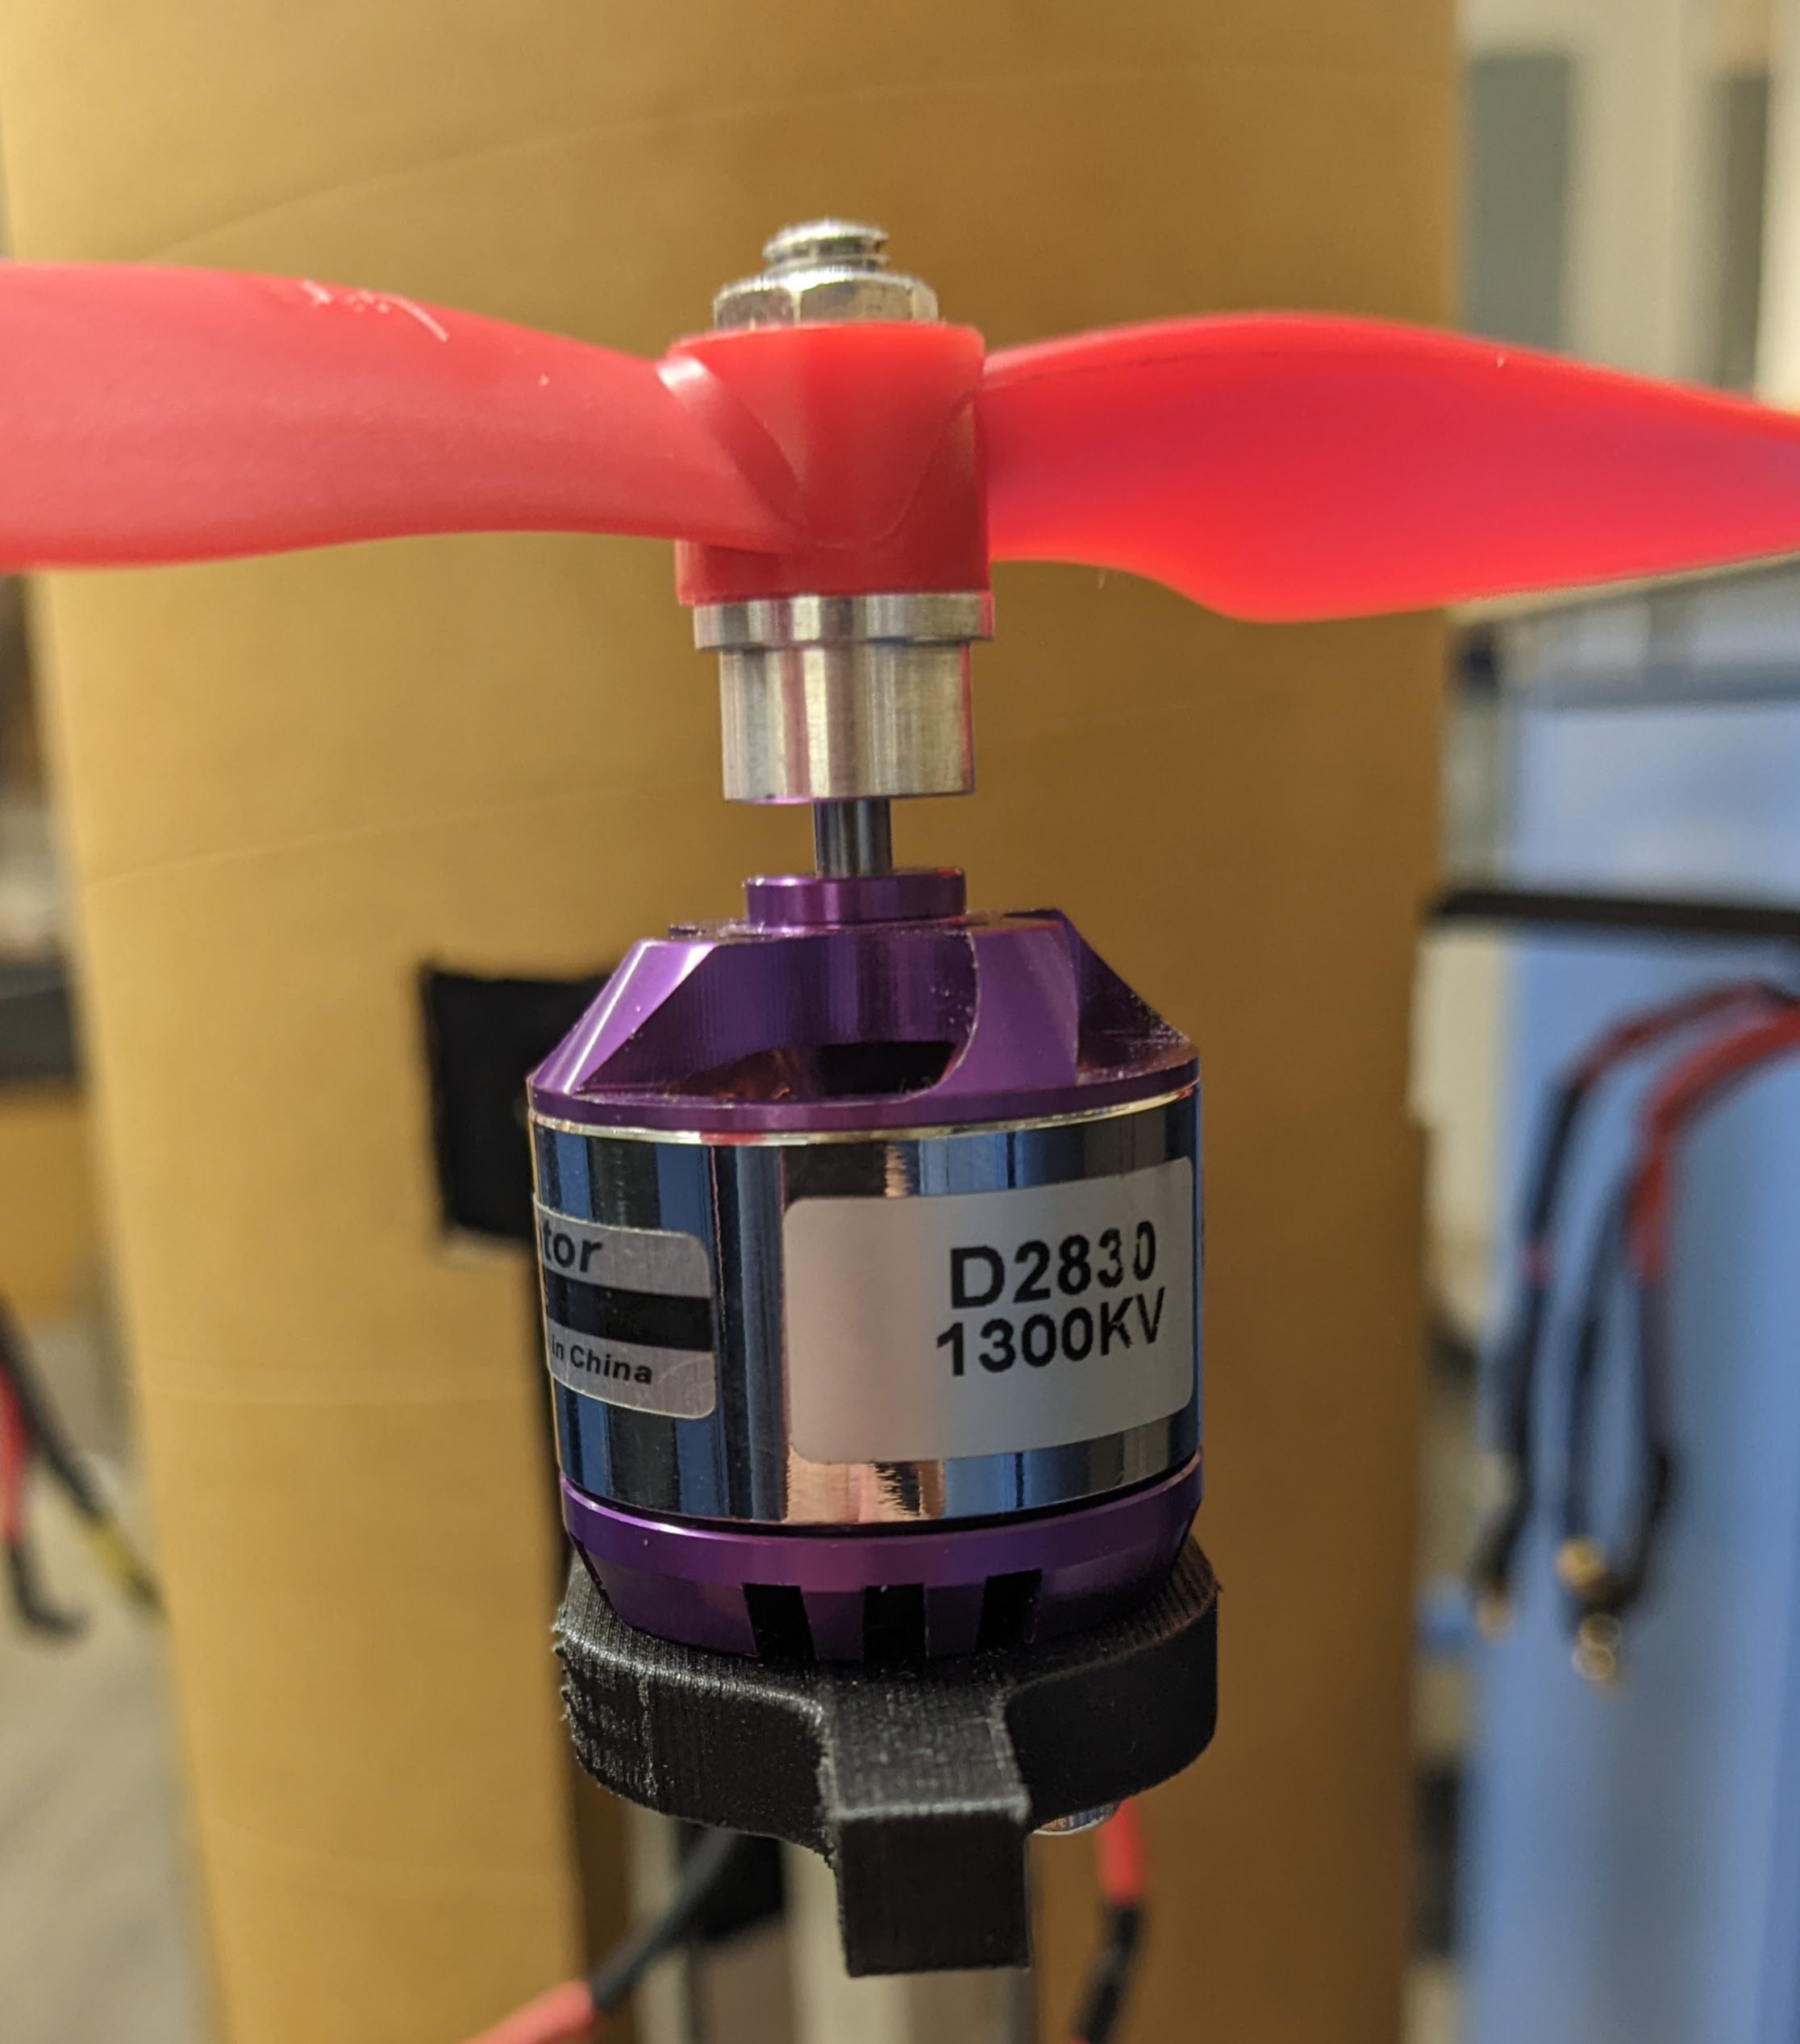
\includegraphics[scale = 0.1]{src/figs/PurpleMotors.jpg}
    \caption{Purple 1300KV motors}
    \label{fig:purple}
\end{figure}

\begin{table}[H]
\centering
% \footnotesize
\caption{Motor Specifications}
\label{design:hardware:esc-table}
\begin{tabular}{|
>{\raggedright\arraybackslash}p{.3\textwidth}|
>{\raggedright\arraybackslash}p{.2\textwidth}|
}
    \hline
     \textbf{Parameter} & \textbf{Value}
    \\\hline 
     Nominal Voltage & 7.4~15V
     \\\hline 
     Instantaneous Maximum Current (10s) & 30A
     \\\hline
     LiPo Compatibility & 2-4S 
     \\\hline
     kv & 1300
    \\\hline
\end{tabular}
\end{table}

\paragraph{Electronic Speed Controllers (ESCs)}

Using the Electronics Speed Calibrators, we are able to get extremely steady RPM of the motors with their very accurate position control. With the candidate motor selected, we were able to move onto finding an compatible ESC. There are a large variety of brushless 30A ESCs. Please refer to the table below for technical specifications of the ESC we chose.

\begin{table}[H]
\centering
% \footnotesize
\caption{ESC Specifications}
\label{design:hardware:esc-table}
\begin{tabular}{|
>{\raggedright\arraybackslash}p{.3\textwidth}|
>{\raggedright\arraybackslash}p{.2\textwidth}|
}
    \hline
     \textbf{Parameter} & \textbf{Value}
    \\\hline 
     Continuous Output Current & 30A
     \\\hline 
     Instantaneous Maximum Current (10s) & 40A
     \\\hline
     LiPo Compatibility & 2-4S 
     \\\hline
     PWM FREQUENCY & 8-18 KHz
     \\\hline
     Mass & 22 g
     \\\hline
     Dimensions & 2.17" x 1" x 0.31"
    \\\hline
\end{tabular}
\end{table}

\paragraph{Batteries}
\label{design:controls:hardware:batteries}
Lithium polymer (LiPo) batteries are by far the most common in the hobbyist drone community due to their high energy density and high discharge rate (figure \ref{fig:lipobattery}). The "S" value is the number of 3.7V (nominal) LiPo cells that are wired in series within the battery. In our case, we elected to use a 3S LiPo battery meaning that there are three 3.7V LiPo cells wired in series for a total nominal voltage of 11.1V.

\begin{figure}[H]
    \centering
    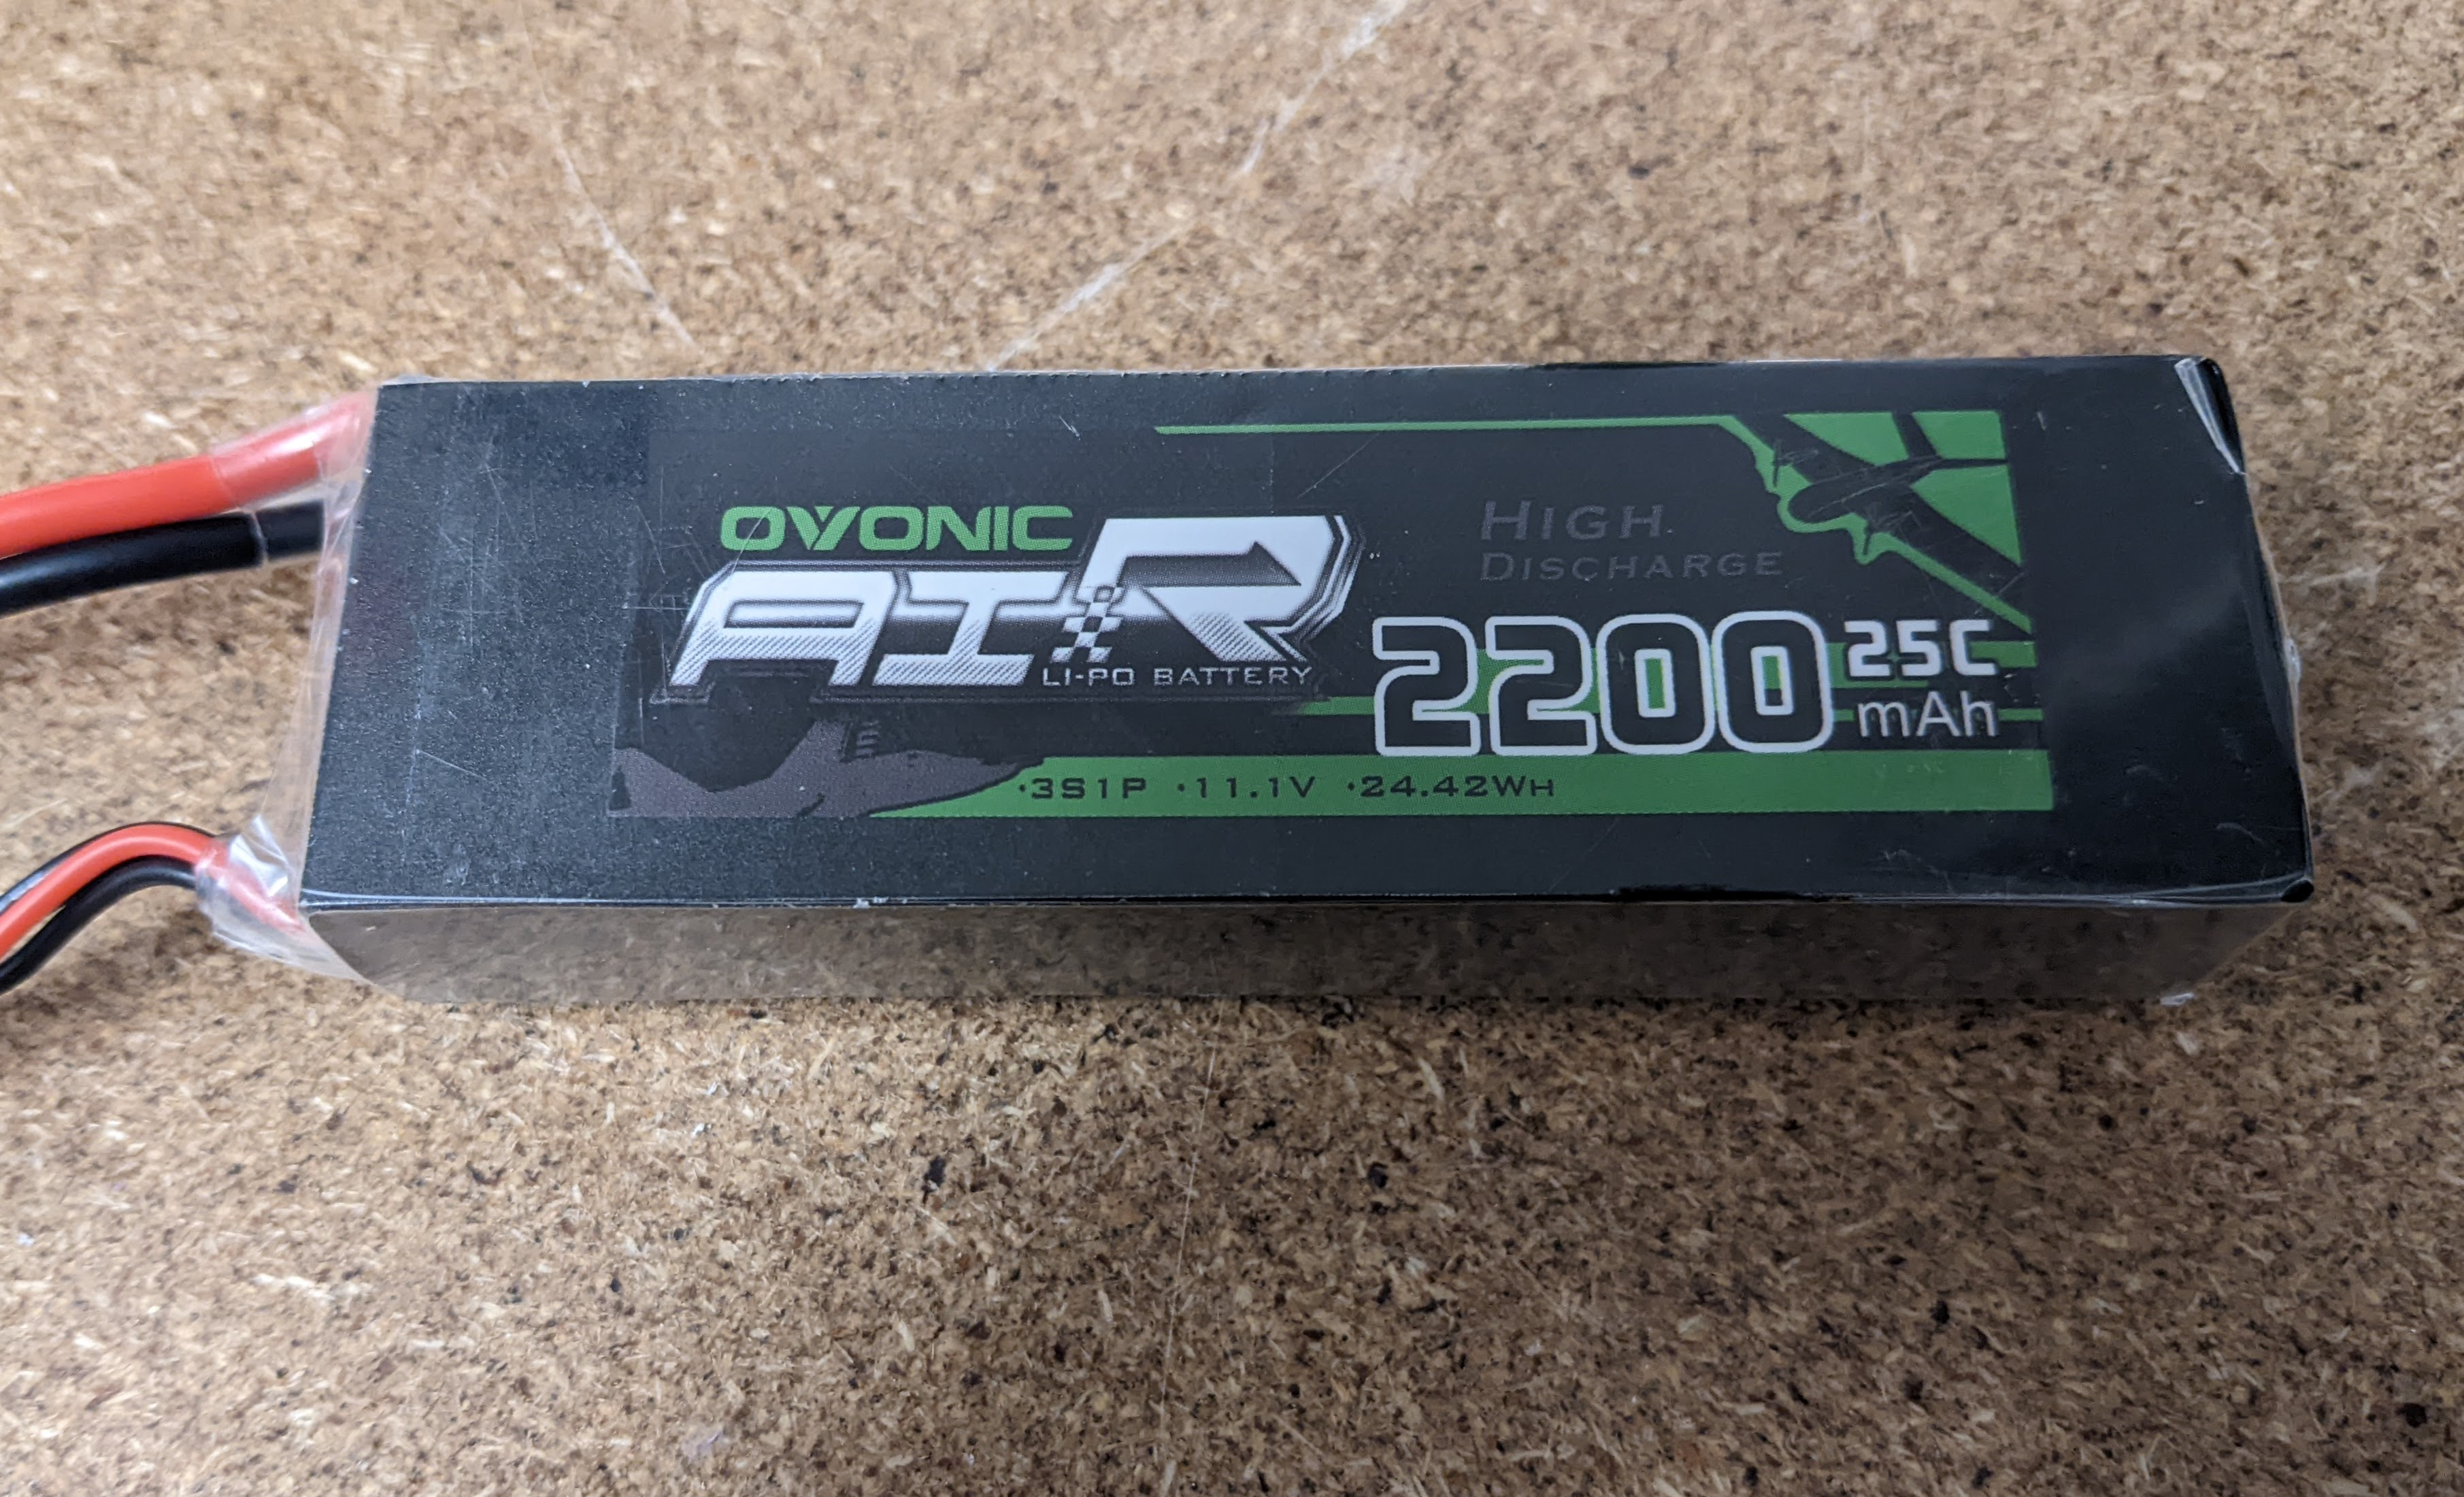
\includegraphics[width=0.5\textwidth]{src/figs/LIPOBattery.jpg}
    \caption{3-Cell Lipo Battery}
    \label{fig:lipobattery}
\end{figure}

The previous motor and ESC selections limited us to the use of 2-4S LiPo's. Choosing a 3S battery was a trivial decision as it gave us balance between increased battery mass and maximum thrust capable of being produces. Please refer to the table below for technical specifications of the battery we chose. 

\begin{table}[H]
\centering
% \footnotesize
\caption{LiPo Battery Specifications}
\label{design:hardware:esc-table}
\begin{tabular}{|
>{\raggedright\arraybackslash}p{.3\textwidth}|
>{\raggedright\arraybackslash}p{.3\textwidth}|
}
    \hline
     \textbf{Parameter} & \textbf{Value}
     \\\hline 
     Battery Type & Lithium Polymer (LiPo)
     \\\hline 
     Total Nominal Voltage & 11.1V
     \\\hline 
     Discharge Rate & 25C
     \\\hline
     Capacity & 2200 mAh
     \\\hline
     Plug & XT-60
     \\\hline
     Mass & 163 g 
     \\\hline
     Dimensions & 4.13" x 1.3" x 0.83"
    \\\hline
\end{tabular}
\end{table}

We also have a dedicated uninterrupted power supply (UPS) battery for the flight computer. UPS is important to protect sensitive electronics on computers. They function by monitoring outgoing voltage and if it dips above or below its nominal threshold, a secondary supply is called upon to return to nominal. Please refer to the table below for the technical specifications of this battery (figure \ref{fig:VGE}).

\begin{figure}[H]
    \centering
    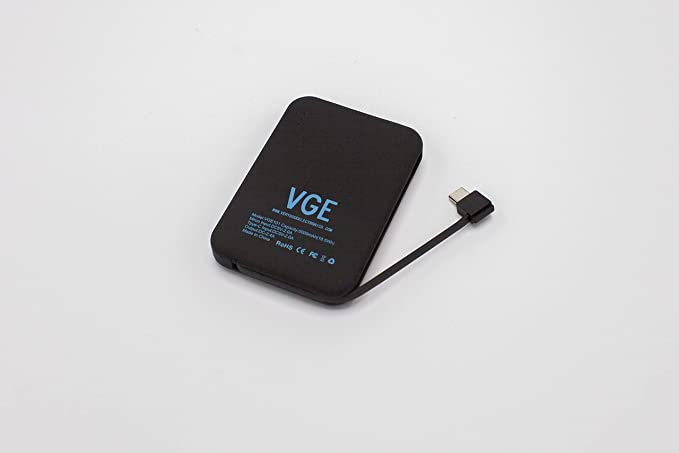
\includegraphics[width = 0.5\textwidth]{src/figs/VGE.jpg}
    \caption{Raspberry Pi Battery}
    \label{fig:VGE}
\end{figure}

\begin{table}[H]
\centering
% \footnotesize
\caption{Raspberry Pi Battery Specifications}
\label{design:hardware:esc-table}
\begin{tabular}{|
>{\raggedright\arraybackslash}p{.3\textwidth}|
>{\raggedright\arraybackslash}p{.3\textwidth}|
}
    \hline
     \textbf{Parameter} & \textbf{Value}
    \\\hline 
     Nominal Voltage & 5V
     \\\hline 
     Output Current & 2.4A
     \\\hline
     Capacity & 4000 mAh
     \\\hline
     Plug & USB-C
     \\\hline
     Mass & 142 g
     \\\hline
     Dimensions & 4.17" x 3.82" x 0.75"
    \\\hline
\end{tabular}
\end{table}

\paragraph{Power Module (PM)} 

The power module (PM) steps down LiPo battery power to 5V for the flight controller and provides full battery voltage to the power distribution board (PDB). The PM is connected to the battery via an XT-60. It feeds power to the Pixhawk via a JST connector and the other end is soldered directly to the PDB. 

\begin{figure}[H]
    \centering
    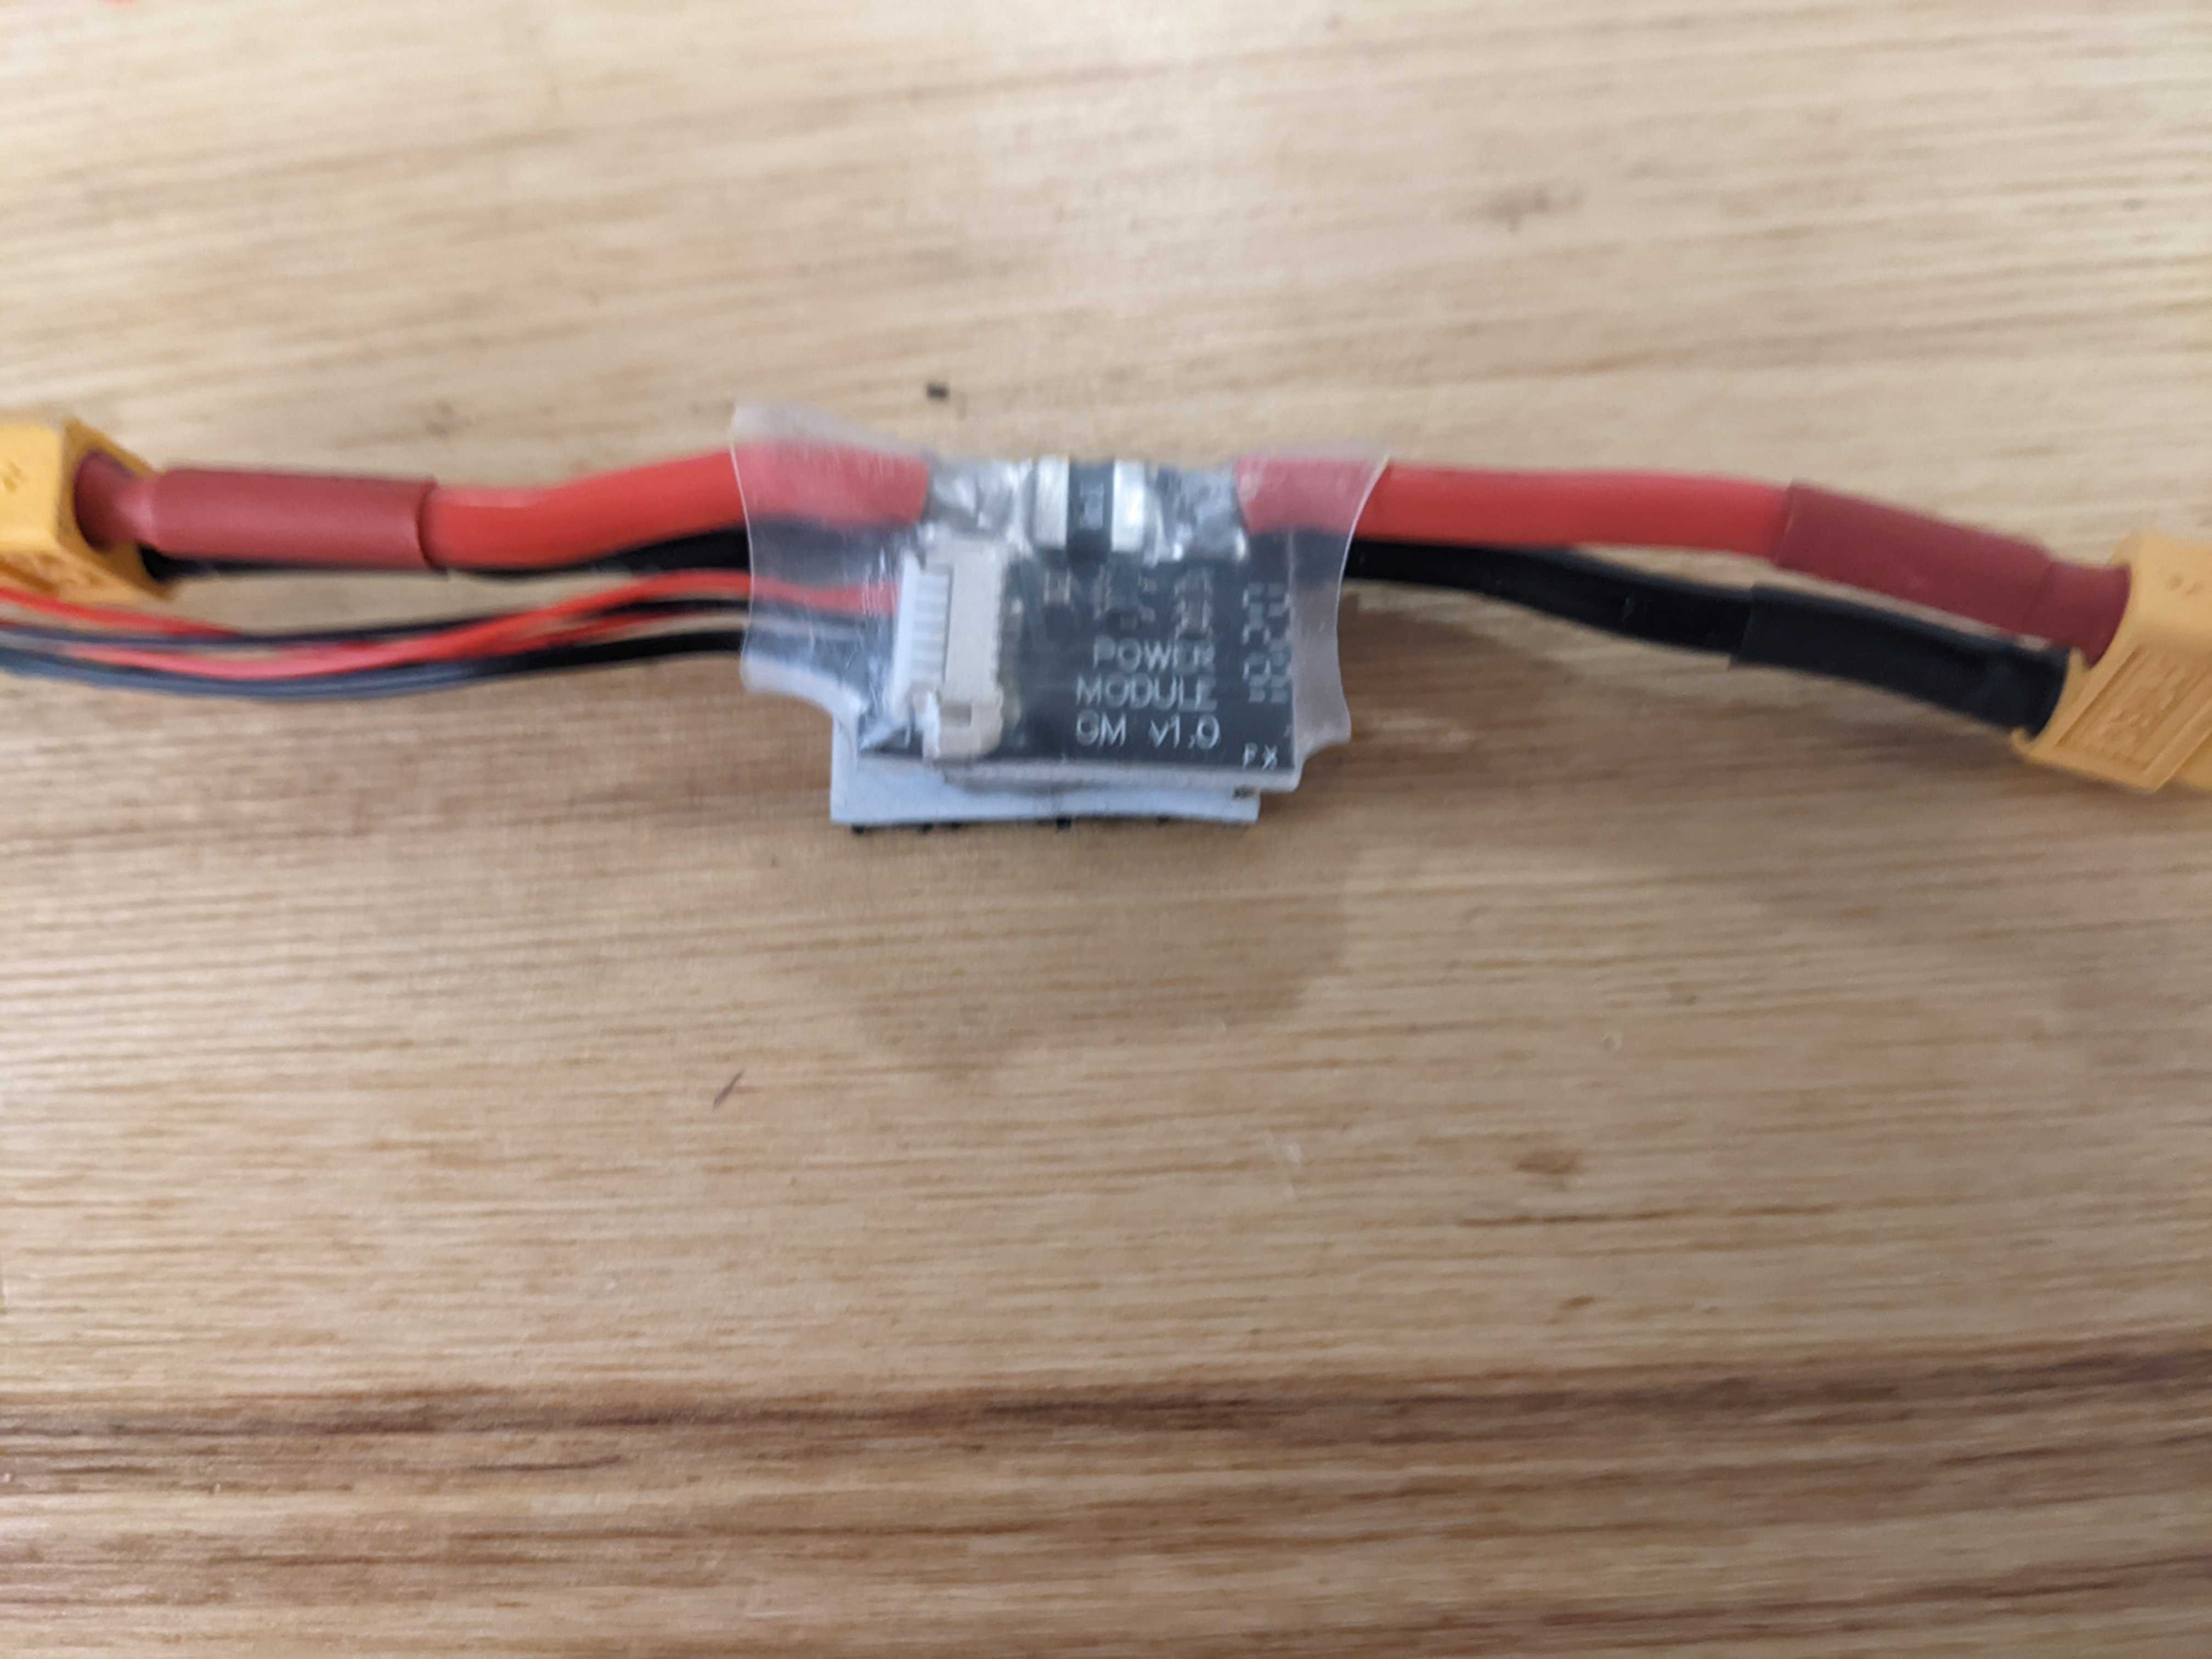
\includegraphics[width = 0.5\textwidth]{src/figs/PM.jpg}
    \caption{PM}
    \label{fig:pm}
\end{figure}


\paragraph{Power Distribution Board (PDB)}

The PDB is a rudimentary printed circuit board (PCB) whose sole purpose is to deliver the full voltage from the battery to all four ESCs without any additional logic circuitry. Copper is used due to its ability to conduct the high current present in our system. An image of ours is shown in figure \ref{fig:PDB}.

\begin{figure}[H]
    \centering
    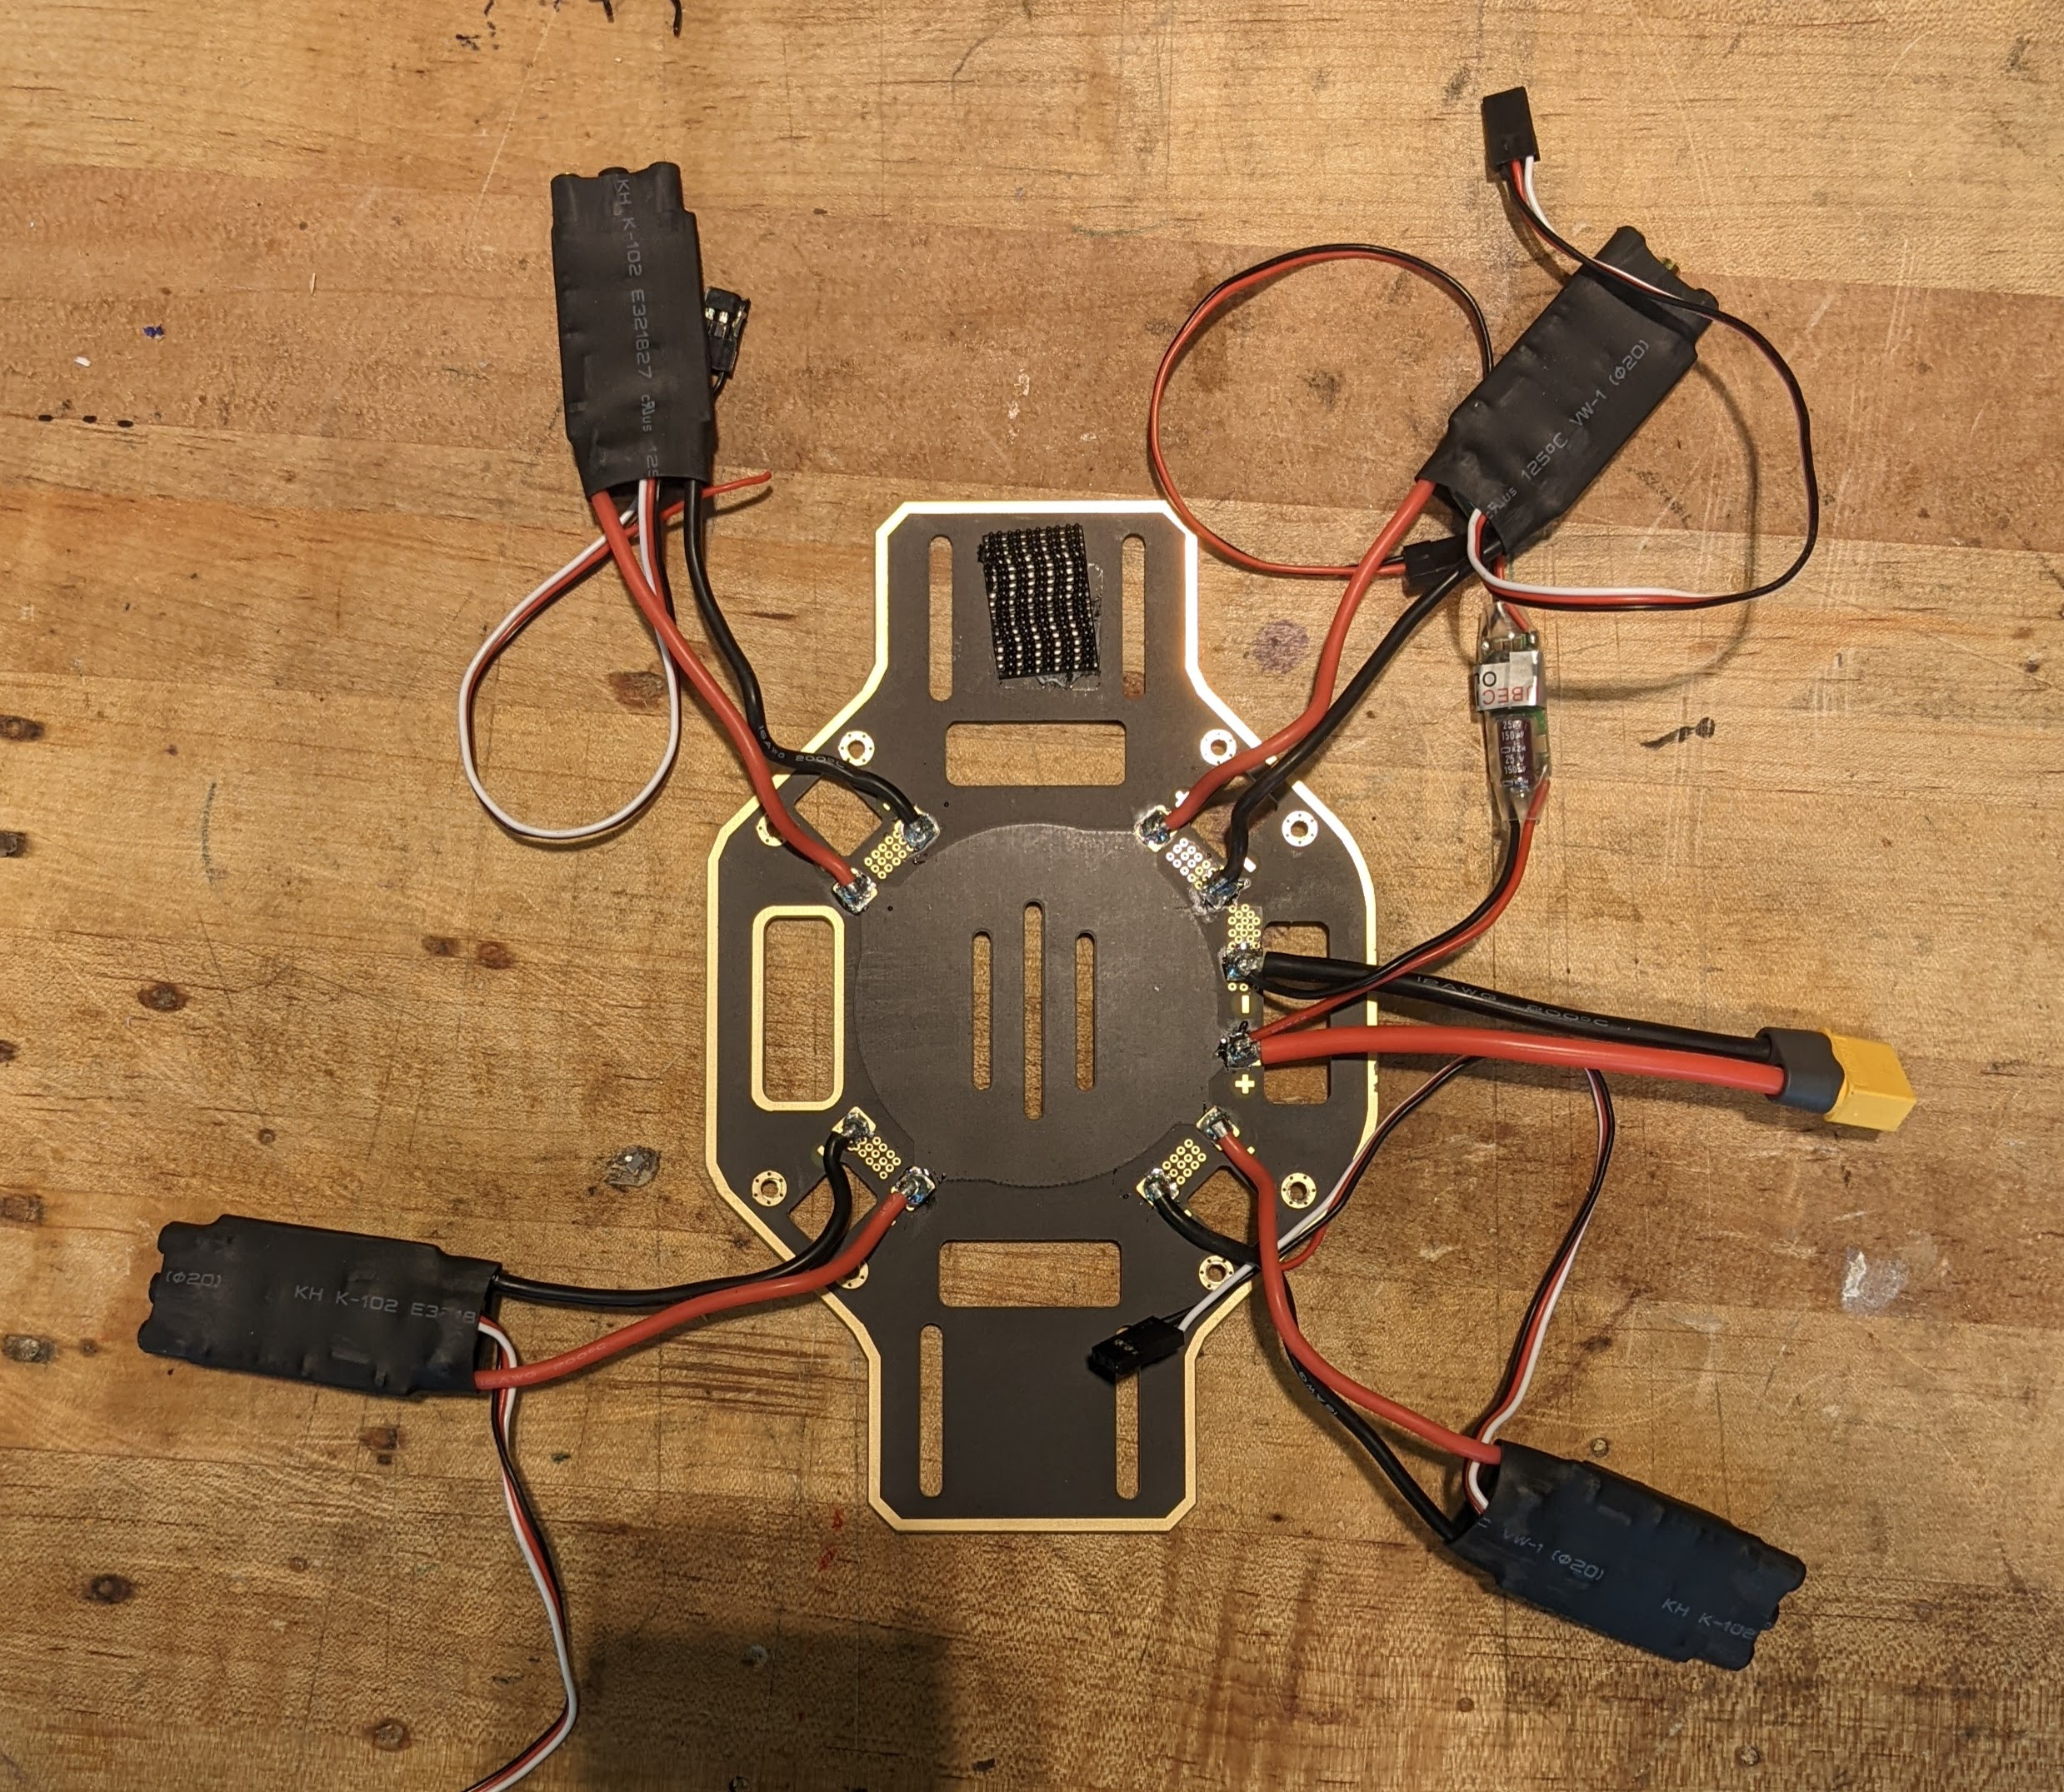
\includegraphics[width=0.8\textwidth]{src/figs/PDB.jpg}
    \caption{Power Distribution Board with ESCs}
    \label{fig:PDB}
\end{figure}

\paragraph{Flight Computer: Raspberry Pi 4 Model B}
In order to add autonomous mission capabilities, we needed an onboard flight computer. The team opted to purchase a Raspberry Pi 4 Model B as the flight computer. The Raspberry Pi was chosen since it is an inexpensive single board computer (SBC) that is commonly used for drones like the one we are building. It is designed to be easy to use for hobbyists, yet powerful enough for advanced projects. The Raspberry Pi 4B came in three different options for memory: 2GB, 4GB, or 8GB. Since the flight computer won't be running any tasks that are unusually computationally intensive, we decided we did not need the 8GB RAM model, however since the price was not that much different from the 2GB model, we opted to go with the 4GB model so we have plenty of RAM in the event that we later decide to incorporate more advanced programs. There are several useful features of the Raspberry Pi that make it a great choice for a flight computer. First, it is able to run the Linux operating system which in turn allows for us to interface with it in a very familiar and easy way. This also enables us to easily connect to the Raspberry Pi over WiFi by using SSH. Connected to the rocket during the mission with SSH is imperative since it allows us to remotely start the main program script which will be discussed later on in Section \ref{design:controls:software}.

Midway through Quarter 2 we ran into a power issue with our flight computer. We were able to SSH into it but it was not capable of sending telemetry signals to the flight controller. We noticed there were no issues when the Raspberry Pi was receiving power from an outlet and came to the conclusion that this was a power issue. We purchased a dedicated battery (See section \ref{design:controls:hardware:batteries}) for the computer and the issue was remedied. 

\paragraph{Flight Controller: Pixhawk} 
In order to control stabilization of the rocket, we decided to purchase a Pixhawk flight controller. The Pixhawk runs ArduPilot firmware and is a all encompassing "black box" solution to drone stabilization. Internal to the Pixhawk are several sensors such as an IMU and a barometer than the ArduPilot firmware uses to stabilize and fly a drone, or in this case, a rotor-powered rocket. The Pixhawk connects to the ESCs that are connected to the motors, so therefore the Pixhawk/ArduPilot is given full control over the flight dynamics of the drone/rocket. Considering the goals of the project as well as the time frame allotted to us, we decided that using the Pixhawk as a black box solution was a sound decision since programming our own stabilization software was not within the scope of the project.

\paragraph{Radio Receiver and Transmitter}
To connect to the drone via the ground station GUI, QGroundcontrol, we used an RC transmitter connected to our laptop through the USB drive. This gave us the capability to connect to a radio receiver/transmitter unit plugged into the Pixhawk flight controller through the SBus pins. This allowed us to monitor the state of the drone during flight, and calibrate all of the sensors prior to takeoff. This was critical to achieving stable flight. Additionally the handheld RC controller could connect to receiver, allowing us to fly the drone manually.

\paragraph{IMU}

The IMU is a peripheral sensor we have included to the system because we could not easily access the acceleration data being from the internal IMU on the Pixhawk. With the external IMU, we are able to read the acceleration of the rocket throughout its flight, letting us detect the drop and collect flight data. The IMU we have chosen, Adafruit BNO055 (figure \ref{fig:theIMU}), has the following specifications:

\begin{table}[H]
\centering
% \footnotesize
\caption{IMU Specifications}
\label{design:hardware:esc-table}
\begin{tabular}{|
>{\raggedright\arraybackslash}p{.3\textwidth}|
>{\raggedright\arraybackslash}p{.5\textwidth}|
}
    \hline
     \textbf{Parameter} & \textbf{Value}
    \\\hline 
     Operating Voltage & 2.4V - 3.6V 
     \\\hline 
     Digital Interface & I2C
     \\\hline
     Pull Rate & 20 Hz
     \\\hline
     Mass & 3g 
     \\\hline
     Dimensions & 0.15" x 0.2" x 1.13"
    \\\hline
\end{tabular}
\end{table}

\begin{figure}[H]
    \centering
    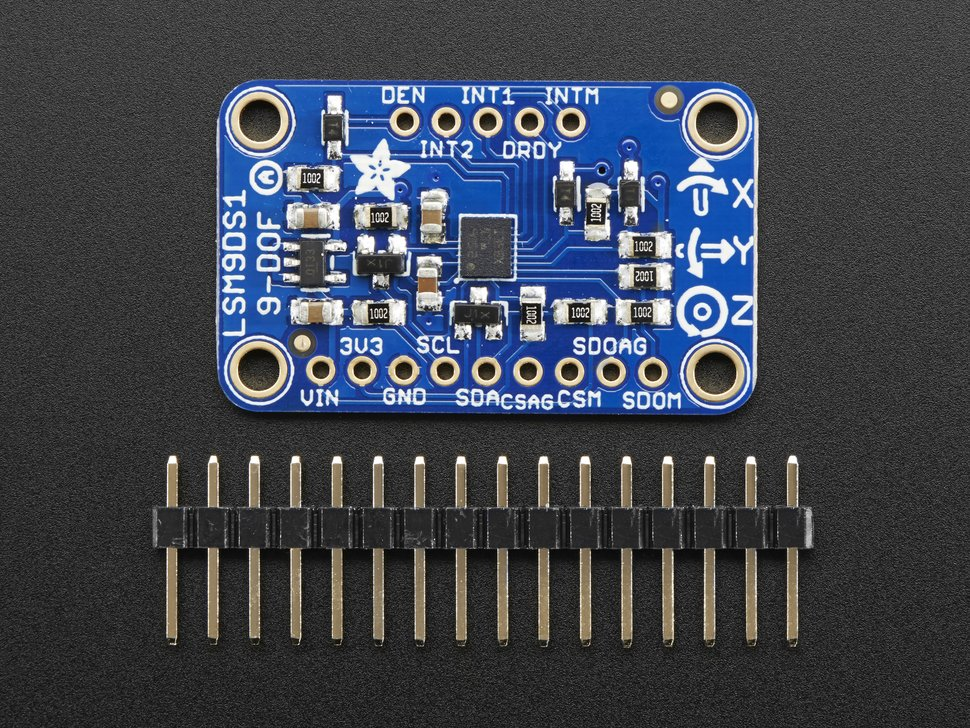
\includegraphics[width=0.5\textwidth]{src/figs/IMU_image.jpg}
    \caption{Adafruit BNO055}
    \label{fig:theIMU}
\end{figure}

\paragraph{Servo}

The arm and leg deployment mechanisms utilize a centralized 35 kg*cm torque rated servo motors, which provides the adequate torque and mount interfaces required for deployment. A servo uses high position controller with a power, ground and PWM input. Our was selected because it can be controlled via a Raspberry Pi and the position of its output spline can be precisely actuated for stowing and deployment operations. Please refer to the table below for the specifications of this motor:

\begin{table}[H]
\centering
% \footnotesize
\caption{Servo Specifications}
\label{design:hardware:esc-table}
\begin{tabular}{|
>{\raggedright\arraybackslash}p{.3\textwidth}|
>{\raggedright\arraybackslash}p{.5\textwidth}|
}
    \hline
     \textbf{Parameter} & \textbf{Value}
    \\\hline 
     Operating Voltage & 5V
     \\\hline 
     Stall Torque (at Locked) & 29 kg*cm
     \\\hline
     Stall Current (at Locked) & 1.9A
     \\\hline
     Mass & 60g
     \\\hline
     Dimensions & 1.58" x 0.79" x 1.50"
    \\\hline
\end{tabular}
\end{table}

\subsection{Software}
\label{design:controls:software}
The software to control the propulsion system is made up of two primary parts: the ArduPilot firmware running on the Pixhawk flight controller, and the Python DroneKit scripts running on the Raspberry Pi flight computer. \href{https://github.com/ArduPilot/ardupilot}{ArduPilot} is an open source autopilot software for drones and other similar vehicles and it is very reputable and well maintained. The DroneKit Python library which is used on the Raspberry Pi flight computer to program autonomous missions is very commonly used in the hobby drone world and offers an easy to use front end for sending MAVLink messages to ArduPilot.

\paragraph{Ardupilot}
As mentioned in Section \ref{design:controls:hardware}, the stabilization and control software used in this project uses several "black box" solutions, and ArduPilot is one of them. ArduPilot, although customizable, handles stabilization and flight dynamics under the hood. It works by taking data from an onboard inertial measurement unit (IMU), and uses a series of feedback loops to control the orientation of the vehicle (in this case quadcopter/rocket).
Considering the time frame and goals, the team decided that developing any form of custom stabilization, flight, or control software outside of ArduPilot was beyond the scope of the project, and ArduPilot was used on the Pixhawk without modification other than basic settings such as number of propellers, 

\paragraph{Scripting Functionality}
The goal of the Python script running on the Raspberry Pi is to interface with an external IMU, as well as the Pixhawk to determine when the rocket is falling, trigger arm and landing leg deployment, and control the rotors to bring the rocket to a hover and land. The main program loop for this code can be found in Appendix \ref{app:main-code} as well as on GitHub: \url{https://github.com/nmarks99/aero-capstone}. 

For reading data from the external IMU connected to the Raspberry Pi over I2C, a Python library from Adafruit's CircuitPython is utilized. In order to ensure consistent readings that do not interfere with the main program loop, the team decided to read IMU data in a separate thread using Python's threading module. Before the main program loop begins, a separate thread is started and from then on, data is read from the IMU concurrently with the main program. To share this data with the main program loop, the IMU data is saved into a mutable array (Python list) that is updated with new IMU values as they are received. At the start of the main loop, the last (most recent) value in the array of IMU data is checked to see if the acceleration is above a threshold value. 

Once drop has been detected, a MAVlink command is sent to the Pixhawk over UART to spin the arm and leg deployment servo using the pymavlink module within the DroneKit library. At this stage, arms and legs are deployed and now the rocket can begin attempting to slow itself down and bring itself to a hover. This is done by setting sending a MAVLink commmand to set the thrust to a maximum value and the thrust will be held at a maximum until the IMU reads that the rocket has reached a hover again. Finally, once hover has been reached, using DroneKit, the vehicle will be set to land mode which will automatically land the rocket below wherever it is hovering at.


\section{Propulsion Arm System}
Of the three main systems that make up the full prototype, the propulsion arm system which underwent the most iterative design process. The Propulsion Arm System development in Quarter 2 was kickstarted by the Quarter 1 Arm Deployment Test Stand (ADTS). The current system is composed of similar components to the ADTS as well as a variety of smaller components that took a rudimentary prototype to a fully functional and reliable system.
\subsection{Propulsion Arms}
The original arms from Quarter 1 on the arm deployment test stand were designed to support a 5" propeller blade. The deployment springs were attached by inserting their legs into two holes drilled into the back of the arm. The arm deployment test stand with the arm attached to it via springs is shown in figure \ref{fig:adts}. Since this initial design the arm has undergone 14 total iterations and 3 significant design changes. 

\begin{figure}
    \centering
    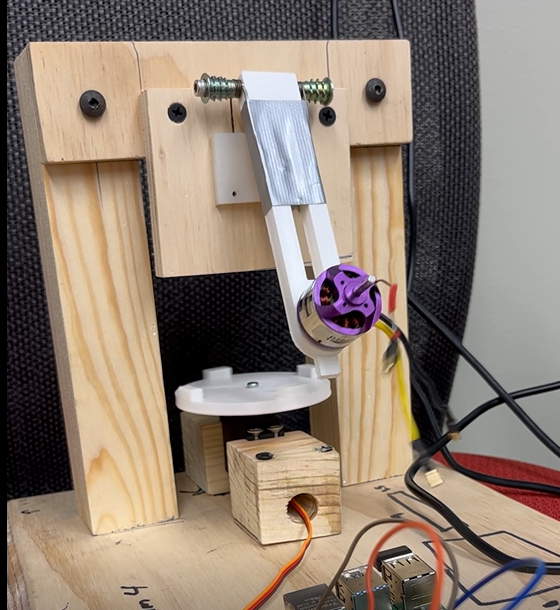
\includegraphics[width=0.5\textwidth]{src/figs/ADTS.png}
    \caption{Original Arm Deployment Test Stand}
    \label{fig:adts}
\end{figure}

In the start of Quarter 2, the team realized that the product would require substantially larger blades than originally planned for. Design of a new arm capable of supporting an 8" propeller blade began and within a week an arm that could be attached to the arm core and support an 8" blade had been modeled and printed. The team worked with this arm size for the majority of the quarter with minor changes occurring including adding 'speed holes' to reduce drag and weight (see figure \ref{fig:speedholes}), reducing arm thickness to reduce mass, and adding ribs along the length of the arm to increase bending strength (see figure \ref{fig:speedholes}). Testing of this arm mainly involved securing 4 of them to the core and working on deployment tests using the pre-deployment locking mechanism and torsion springs. It was found that the arm deployed quickly but once deployed it had the ability to both slide side to side in the bay but also twist. It was determined that this was a result of using bolts that did not provide a tight enough fit between the arm and core.

\begin{figure}
    \centering
    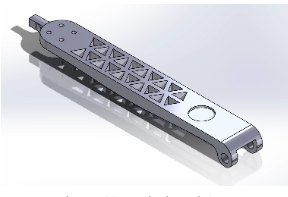
\includegraphics[width=0.5\textwidth]{src/figs/armwithspeed.png}
    \caption{Speed Holes on arm}
    \label{fig:speedholes}
\end{figure}

The second serious design change came when the team realized that 8" blades would no longer provide the thrust needed to support our platform. This realization came with a redesign of the arm to support 10" blades. This involved lengthening the arm as well as performing a new ANSYS simulation to ensure that the arm would still be able to withstand the moment caused by the thrust. This arm was attached to the core for testing using 1/4" shoulder bolts as opposed to the M6 bolts found in the Ford Prototyping Shop and to further prevent side to side motion, the core end of the arm was widened to reduce total clearance with the bay walls from 0.15" to 0.05". These two changes proved successful in better securing the arm and eliminating twist according to observations made.

The third and final serious design change came with the final selection of the motor and propellers that are used on the alpha prototype. The larger, 2830 stator size motors were significantly taller than the previous motors that were used for testing. To allow these motors to still fit within the diameter of the 6" rocket body, a 5/8" step-back was added to the arm. This allowed the core to remain unchanged while allowing all components to fit inside the rocket body. The final arm can be seen in figure \ref{fig:newarm}.

\begin{figure}
    \centering
    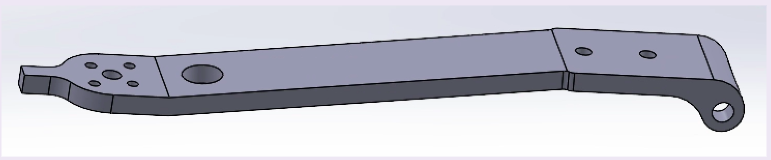
\includegraphics[width=0.75\textwidth]{src/figs/finalarm.png}
    \caption{Final Arm Design}
    \label{fig:newarm}
\end{figure}

The stepped-back arm design is the propulsion arm currently in place on the alpha prototype. This arm is capable of supporting blades up to 10" in diameter, allowing for 1/2" clearance from the rocket body when fully deployed. This arm mounts to the central core, discussed in coming sections using a 1/4" shoulder bolt that passes through it on the underside as well as through both bay walls on the core. Additionally, the arm is capable of supporting any motor that has a 16mm x 19mm mounting pattern that is less than 2" in total height with a mounted propeller. It was critical that the propulsion arm was incredibly stiff since it would be undergoing the largest loading of any component in the entire prototype. To get a component this stiff while keeping it as light as possible, it was 3D printed using Onyx with carbon fiber inlay. This material has the bending stiffness of 6060 T6 Aluminum, and when modeled in ANSYS, the arm deflected less that 1 millimeter under loading with a 1.5 Factor of Safety. For more information on this ANSYS simulation, please see section \ref{propulsionarmansys}. In addition to the motor mount, the final propulsion arm also incorporates the following features.

\begin{itemize}
    \item Pre-Deployment Locking Mechanism Interface Tab
    \item Through Hole to allow motor wires to pass to underside of arm
    \item (2) countersunk M3 screw holes for deployed locking mechanism attachment
    \item (2) shoulder bolt supports for attachment to the core
    \item (2) torsion spring alignment slots
\end{itemize}

\subsection{Deployment Method}
In Quarter 1, the team researched propulsion arm deployment methods. The most defining requirement for the arm deployment mechanism was that it was quick to prevent the rocket from gaining too much velocity and impacting the ground before it could be slowed. A variety of options were researched including a geared system, servos, hydraulic springs, and torsion springs. The geared system and hydraulic springs were eventually eliminated from the selection process as both would either be too heavy or too complex to implement in a small scale, amateur rocket. Of the remaining two contenders, the servos were explored first. The team purchased two servos that were believed to have a torque sufficient to lift our initial arm prototype 90 degrees. It was found that the smaller of the two servos was not only too slow, but also not strong enough to fully lift the arm, which was 1/4 the size of our alpha prototype arm. After this test, the team decided to move away from the use of four servos in an effort to minimize weight and power requirements. With servos now eliminated, torsion springs were the leading concept. Several springs of varying spring constants were purchased and tested. Due to their quick, reliable, and simple nature, torsion springs were selected as our final propulsion arm deployment method. Initially, the team was using 2, 90 degree torsion springs on each arm. One left hand wound and one right hand wound spring on each arm. However, it was found that despite having a 90 degree free angle, their range of use before plastic deformation was limited to about 60 degrees of compression. As a result of this discovery, the team switched to using 120 degree torsion springs. Double torsion springs were briefly looked into but it was found that no double torsion springs that were narrow enough to fit under the arm would provide a spring constant high enough to fully deploy the arm. As previously stated, the team decided to use two, 120 degree torsion springs on each arm. This would allow the spring to compress 90 degrees while staying in its elastic deformation regime. The selected springs are for a 0.296" shaft and have a maximum torque of 3.54 in-lbs at their fully compressed position.


\paragraph{Pre-Deployment Locking Mechanism}
\label{pre-deployment_arm}
To complement the selection of torsion springs as the propulsion arm deployment method, a mechanism that blocked the arms' path of travel would be required since the torsional springs cause the arm to naturally want to deploy. In effort to reduce mass, the team wanted to proceed with a mechanism that worked for all four arms simultaneously as opposed to having a mechanism for each arm. The team came up with two leading ideas, each of which involved an 'unlocking disk' that was actuated through the use of a single servo. The first design latched with four doors that would be situated on the outside of each arm bay. Inside the rocket, the torsion springs would be pushing the arm against the inner face of the door. When rotated, the disk would unlatch the door allowing the arms to push the door open and fully deploy. The second idea followed similar suit but instead, latched the arms inside the rocket as opposed to the latching doors. It did this by being situated below the stowed arms and having four tabs that stuck vertically out of its surface. These tabs were at a diameter so that when the arms were vertically stowed, the tabs would interface with the end of the arm, blocking their travel. Design idea \#1 was selected by the team to proceed with since it combined two functions, securing the bay doors, and securing the arms. A CAD model was quickly made so the idea could be demonstrated to the professors in our next meeting. These can be seen in figure \ref{fig:diskdoor} and \ref{fig:doorlatch}. However, in that meeting with the Capstone Professors, they advised us that designing a system that combined the two functions was too ambitious and instead heavily recommended that we proceed with design idea \#2. This idea was then completely redone in SolidWorks to begin printing and testing.

\begin{figure}[H]
    \centering
    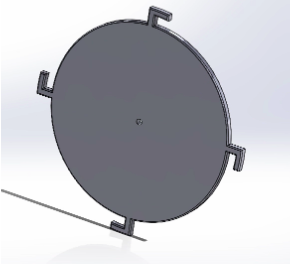
\includegraphics[width=0.5\textwidth]{src/figs/doordisk.png}
    \caption{Final Arm Design}
    \label{fig:diskdoor}
\end{figure}
\begin{figure}[H]
    \centering
    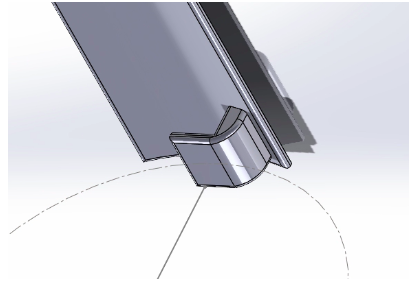
\includegraphics[width=0.5\textwidth]{src/figs/doorlatch.png}
    \caption{Final Arm Design}
    \label{fig:doorlatch}
\end{figure}

Quarter 1 ended with the team having a functional propulsion arm deployment system involving a small arm, 2 torsion springs, and an unlocking disk mounted below the stowed arms which spun when a servo was commanded to rotate. The quarter one prototype, also known as the Arm Deployment Test Stand (ADTS), can be seen in figure \ref{fig:adts}.


Since this initial Quarter 1 prototype, design of the pre-deployment locking disk has remained nearly the same. Changes were made to the diameter of the disk and the positioning of the tabs in accordance with changes to arm thickness and position within the rocket body. These changes were only a matter of redefining dimensions in the SolidWorks part and reprinting. The first real change came late in Quarter 2 after increasing the torsion springs spring constant. With the added torque from the springs, the team noticed during testing that the servo was spinning but the disk was not. It was found that this was a result of the M3 fastener that secures the disk to the servo slipping from the added torque. To remedy this problem, one of the provided attachments for the servo was attached and a small extruded rectangular cut was made in the bottom of the disk. This allows for the servo attachment to rotate with the servo, preventing slipping. This cutout can be seen in figure \ref{fig:cutout} This change completely fixed the problem and the design of the unlocking disk did not change until just before the alpha prototype. 

\begin{figure}[H]
    \centering
    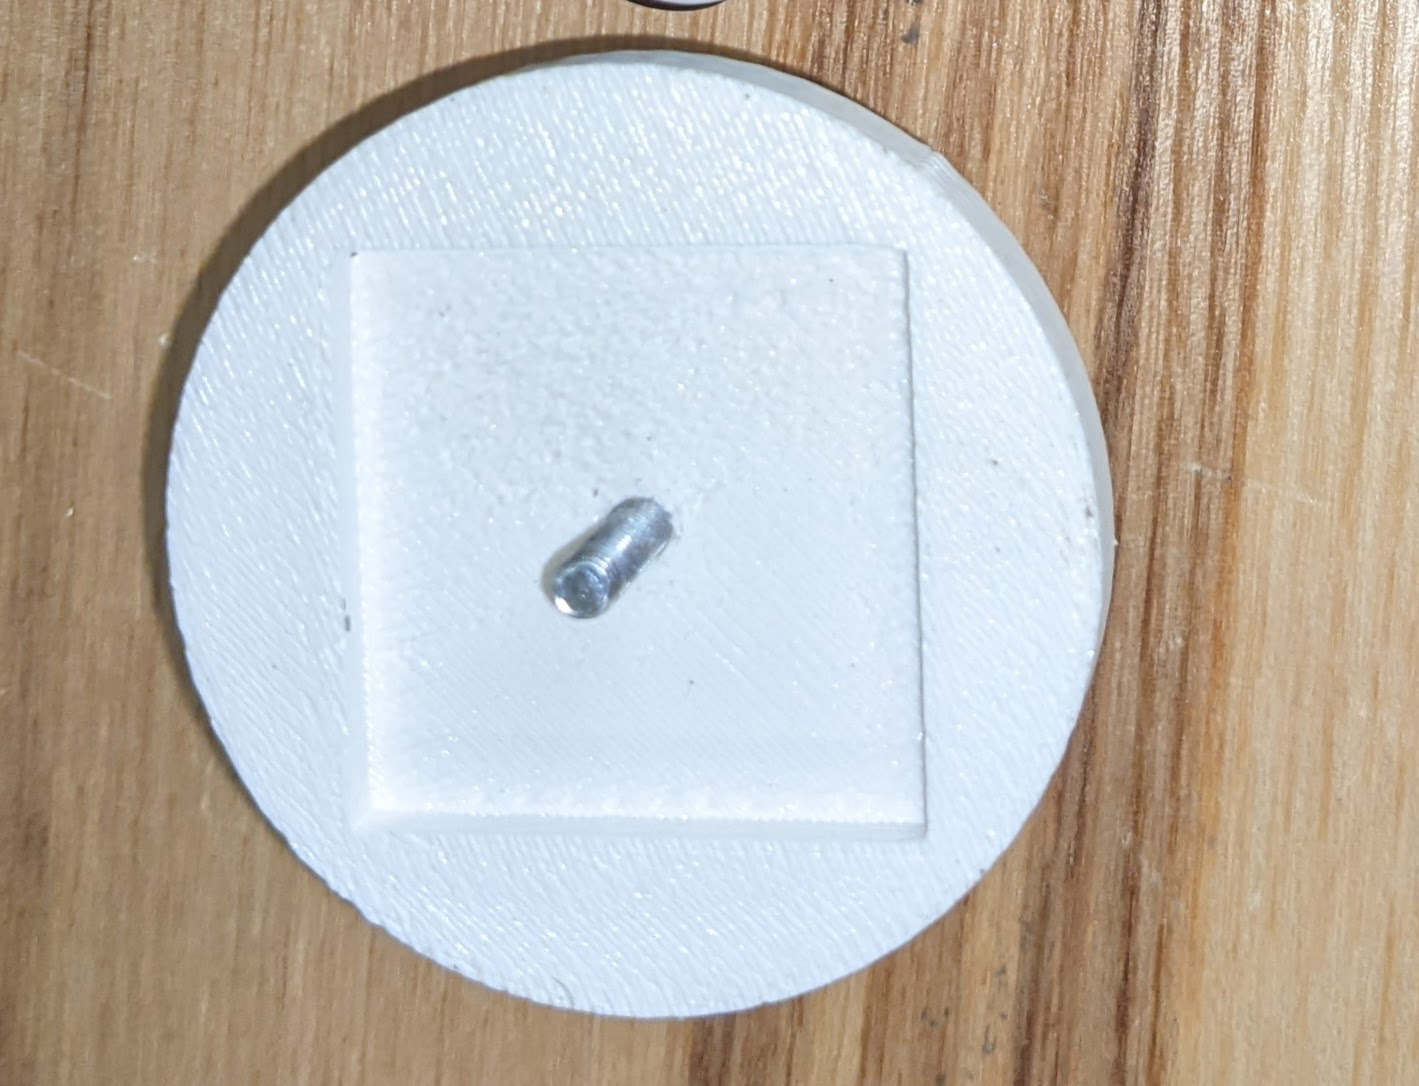
\includegraphics[width=0.5\textwidth]{src/figs/Spool_Cutout.jpg}
    \caption{Cutout to Prevent slipping}
    \label{fig:cutout}
\end{figure}

With the end of the quarter approaching and the entire alpha prototype designed and built, the team began a tedious process of mass reduction. In this process, it was found that both the legs and arms could be deployed simultaneously. Previously, one servo was used for arm deployment, and one was used for leg deployment (more on this in following sections). In order to reduce mass, the team elected to combine these functions and instead use one servo for both arm and leg deployment. To accommodate this change, a long stem was added to the bottom of the pre-deployment locking disk, this allowed it to nest with the leg pre-deployment locking mechanism, discussed later. They nest via a 0.25" hole in the bottom of the disk stem using M2 threaded inserts and screws. Concurrent with this change, the diameter was changed one final time to accommodate the alpha propulsion arms which involved the step-back design which greatly reduced the size of the disk (1.25" diameter reduction). This design is present in the alpha prototype and is 3D printed using ABS. Figure \ref{fig:extendeddisk} shows the extended disk. Figure \ref{fig:combined attachments} shows the two combined pieces. 

\begin{figure}[H]
    \centering
    \includegraphics[width=0.3\textwidth]{src/figs/extendeddisk.png}
    \caption{Extended Disk}
    \label{fig:extendeddisk}
\end{figure}

\begin{figure}[H]
    \centering
    \includegraphics[width=0.2\textwidth]{src/figs/combinedattach.png}
    \caption{Combined Servo Attachments}
    \label{fig:combined attachments}
\end{figure}

\paragraph{Servo Holder}
To secure the servo for arm deployment in place, the team designed a servo holder (figure \ref{fig:SH}). This holder was a single piece that slid over the inner rails of the support structures (discussed in following sections). It had a box that provided a tight fit with the servo in the center of it that would allow the spindle of the servo to be perfectly centered in the rocket. This design was printed out of ABS and worked well for testing. However, it was later combined with another component during the mass saving process and does not present itself in the alpha prototype. This combination will be discussed in the section detailing the design of the inner assembly support plates.

\begin{figure}[H]
    \centering
    \includegraphics[width=0.75\textwidth]{src/figs/ServoHolder.jpg}
    \caption{Servo Holder}
    \label{fig:SH}
\end{figure}


\paragraph{Deployed Locking Mechanism}
\label{armdeployedlockignmechanism}
Once deployed, the arms need to stay fully deployed to prevent a moving center of thrust, and possibly a blade strike with another component. Several solutions were investigated and the first one selected for testing involved the use of high-strength Neodymium magnets. Magnets were selected due to their fairly cost effective price, reliability (won't fail magnetically), and simplicity of design and installation. Calculations were performed to select magnets that would have the strength to support the moment of the arm and the motor, and magnets that met these specifications were selected. Once ordered, the propulsion arms were modified with a small 11/16" diameter, 1/16" deep circular cutout on the top surface of the arm where it interfaces with the core. This would be the location in which the arm magnet was secured. An accompanying magnet would be secured to the core just above where the arm magnet would fall in the deployed position. The magnets were attached to the arm and core and testing began. The slot for the magnet can be seen in figures \ref{fig:armwspeed}. Initial testing was promising, the magnets were as strong as we expected and could easily hold the arm and motor. Despite this early success, problems arose with the magnets during deployment testing. It was found that if the magnets were not perfectly aligned, when the propulsion arm struck the core magnet, it would bounce off since the magnets did not meet flush. This resulted in fairly serious oscillations of the arms that lasted up to several seconds. After these tests, the magnet idea was scrapped and the team began researching new methods. 

\begin{figure}[H]
    \centering
    \includegraphics[width=0.75\textwidth]{src/figs/armwithspeed.png}
    \caption{Arm with Magnet Slot}
    \label{fig:armwspeed}
\end{figure}

Two promising ideas were quickly developed and printed for testing. The first idea involved a protrusion from the core that would allow the arm to move into the locked position but not the other way. The second idea involved the use of a spring plunger pin. The pin would be secured to the arm and held in its compressed position while the arm was stowed. Once deployed, the pin would run along the arm bay wall of the core before deploying into a cutout when the arm reached its fully deployed position. Since this mechanism was only concerned with not letting the arm fall, the team was not concerned with the loading it would take since the thrust force would not be sent into it and instead into the core. The pin would be secured to the underside of the arm using a press fit holder that would attach to the arm via two small bolts. After printing new cores that would accommodate these mechanisms, both were tested. It was found that design \#1, the core tabs, was too stiff and too brittle. When deployed, the arm did not pass through the tabs and if pushed through, the tabs would crack. Design \#2, the spring pin, was found to work great and reliably locked the arms in the deployed position (more on testing in the testing section). Design \#2 was selected for further development. The deployed position of the mechanism can be seen in figure \ref{fig:armlocked}.

\begin{figure}[H]
    \centering
    \includegraphics[width=0.75\textwidth]{src/figs/deployedarmimageview3.png}
    \caption{Locked Arm Position}
    \label{fig:armlocked}
\end{figure}



For iterations of this locking mechanism, changes to the initial spring pin design were minimal, and only involved reducing the core cutout size to prevent any vertical motion of the arm and adding countersunk M3 holes to the arm to secure the spring pin holder to it. This design is present in the alpha prototype. 

\subsection{Core}
From the mid-point of Quarter 1, the team decided that simplifying assembly and disassembly would be helpful for maintenance and replacement of internal components. However, it wasn't until Quarter 2 that development of a mechanism to fulfill this requirement began. The initial design was made of 4 propulsion arm bays. These bays were 1.5" wide and consisted of three vertical walls and one top surface. The two side walls were in place to prevent the propeller blades from rotating before deployment. The third vertical wall was located more central than the arms inside the rocket. This wall provided a surface for the other end of the torsion springs to push against to deploy the arms. Finally, the top surface provided a support for the arm so it could not travel beyond its fully deployed position. The design had two holes in each bay to allow a fastener to pass through and secure the arm in its place in the core. Additionally, two supports were added to the exterior faces of two of the walls with a 1/4" through hole to allow the core to mount on 1/4" threaded internal rails (discussed in coming sections) to allow for easy removal.

Since this design, the concept of the core has remained nearly identical with four bays each made of three walls and a top surface. The most drastic design change came with the switch from 90 degree to 120 degree torsion springs for arm deployment. The team wanted the springs to be at their free angle when the arms were fully deployed. To allow for this, the inner walls of the core were slanted 30 degrees towards the center so that when the arm is deployed to its 90 degree deployed positions, the springs are in their 120 degree position. In addition to this change, small tabs were added to the slanted face to prevent the springs from slipping out of place which could prevent proper arm deployment. Additional changes have included narrowing the bays from 1.5" to 1.25", shortening the vertical walls and instead adding 'blockers' that extend below the core to prevent rotation of the blades, and adding the cutouts for the propulsion arm deployed locking mechanism. The alpha prototype is 3D printed using high infill ABS. Each bay provides structures to support the propulsion arm, the deployment method, and the deployed-locking mechanism. Additionally, the extra space on the walls of the bays and top surface are used for mounting the electronic speed controllers as well as the power distribution board.

\paragraph{Avionics Sled}
To support the remaining avionics, a flat plate was printed that could be mounted vertically inside the rocket body on the internal support structures. This component was originally 4.5" wide and 6" tall (figure \ref{OES}. In the mass saving process, this component would be combined with the lower support plate, discussed in the following section. 

\begin{figure}[H]
    \centering
    \includegraphics[width=0.5\textwidth]{src/figs/OldElectronicSled.jpg}
    \caption{Original Electronics Sled}
    \label{fig:OES}
\end{figure}


\subsection{Inner Assembly Support Plates}
To facilitate easy removal of internal components, the team designed a system that would combine all internal elements into one module that could be put in or out of the rocket body all at once and then the individual components could be disassembled. This module involved using two support plates and two threaded rods. The two support plates were 6" in diameter to match the inner diameter of the rocket tube. They each had two, 1/4" holes. The threaded rods for mounting the components passed through these holes and were secured on both sides with shouldered nuts. along the outer face of each plate, 8 pilot holes were printed. These holes were expanded and M3 threaded inserts were added to secure the plates to the rocket body. They were secured by passing M3 screws through the body tube and into the plates. Connecting the two plates, were two, 1/4" threaded steel rods. All internal components were slid onto these rods and secured using shouldered nuts. This system remained unchanged until the mass saving process. At the end of Quarter 2, to reduce mass, the threaded 1/4" steel threaded rods were swapped for \#10-32 aluminum threaded rods. This reduced the mass of the rods by approximately 25\%. Additionally, the upper support plate was combined with the avionics sled and the lower support plate was printed to accommodate the leg and arm deployment servo. The alpha prototype is made of two support plates, one that houses the avionics and one that houses the deployment servo. These plates are connected by two \#10-32 rods and secured to the rocket using 16, M3 screws.

\section{Landing Leg System}
The Landing Leg System was the final of the three main systems to enter the design stage. Development of the landing legs began around week 15 of the project. Numerous designs were developed, tested, evaluated and either scrapped or iterated on. The final landing leg assembly is shown in Figure \ref{figs:legassemble}. 

\begin{figure}[H]
\centering
\includegraphics[scale=0.7]{src/figs/overviewlandinglegpiclabeled.png}
\caption{Alpha Prototype of the Landing Legs with Labels}
\label{figs:legassemble}
\end{figure}

The purpose of the landing legs is to support the rocket body upon landing and ensure that the rocket body lands upright in a stable position. The needs that the landing legs must meet are \#3, the ability to stand upright on its own, \#7 reproducible on a college club budget, \#8 structural stability, and \#12 deployability. The team broke down the landing leg design into three separate functions: structural design for load bearing and landing upright, deployment of the legs from an initial stowed position, and two different locking mechanisms to lock the legs in their stowed position and their deployed position. These separate functions were brainstormed and ranked independently. Once solutions that best met the mission's needs were highlighted, they were combined with the other function's solutions and ranked once again. 
The following sections detail this process and what steps were taken to get to the alpha prototype.

\subsection{Structural Leg Design}

The structural leg design investigated different deployment motions and load-bearing structural components that would minimally interfere with the rocket body and other mechanical and electrical components, allow for quick deployment, minimize stress at concentration points, and have minimal complex geometries and manufacturing techniques. A common landing leg design in the aerospace industry includes a primary strut that acts as the main load-bearing element and a secondary strut that provides additional support especially in the axial direction. The other possible design that fit our project includes a single load-bearing strut. The deployment motions possible with these designs include rotation that is tangent to the rocket body, deployment outwards using the bottom of the rocket body as a hinge/rotation point, stowing the legs inside of the rocket body and deploying them from the bottom outwards, and deploying the legs outwards from the upper section of the rocket body (Figure \ref{figs:dm}).

\begin{figure}[H]
\centering
\includegraphics[scale=0.8]{src/figs/deploymentmotions.png}
\caption{Deployment motions}
\label{figs:dm}
\end{figure}

The needs of the landing leg design highlighted above indicates that the primary-secondary strut solution was best fit for the project mission because it is simple, distributes forces on two connection points to the rocket body which reduces shear stress, and reduces bending stress when compared to a single strut while increasing the rocket's stability/footprint. The deployment motions that best meet the landing leg's needs are ideas 2 \& 4. Idea 1 limits the geometry of the strut, sacrifices stability, and would likely interfere with other components when rotating about its axis. Idea 3 causes the legs to be directly in the path of a theoretical thruster, making it unacceptable for the NUSTARS project application. Ideas 2 \& 4 are best suited to the project. The next step in designing the landing legs was to investigate and select potential solutions for the deployment method.

\subsection{Deployment Methods}

The deployment method directly meets the deployable need of the legs outlined above. It is a mechanism that provides a force to initiate the motion of the legs from their stowed position to their final deployed position. The deployment method needs to be lightweight, simple, quickly able to deploy the legs, need minimal support from additional structures, reusable, reliable, and able to apply a sufficient force (or energy) to deploy the leg. The potential solutions and their scores against each need are shown in Figure \ref{figs:dmam}.

\begin{figure}[H]
\centering
\includegraphics[scale=0.7]{src/figs/deploymentmethodalternativesmatrix.png}
\caption{Deployment Methods Alternatives Matrix}
\label{figs:dmam}
\end{figure}

The two solutions that ranked the highest are to torsion spring and linear spring. Next, the general locking mechanism was investigated. 

\subsection{Locking Mechanism}

The locking mechanism refers to the component of the landing legs that constrain the motion of the leg before and after deployment. Similar to the deployment mechanism, the needs are lightweight, simple, minimizes stress at connection points, locks the legs quickly, minimally supported by additional structures, reusable and reliable. 

\begin{figure}[H]
\centering
\includegraphics[scale=0.8]{src/figs/lockingmechanismalternativesmatrix.png}
\caption{Locking Methods Alternatives Matrix}
\label{figs:lmam}
\end{figure}

Figure \ref{figs:lmam} shows the best solutions are a structure that blocks the path of travel of the landing leg and the use of a spring loaded pin. 

The next step was combining these functions and top potential solutions into a single landing leg design and ranking them. 

\subsection{Landing Leg Configurations \& Mockups}

Different combinations of solutions were combined into landing leg configurations and ranked according to how they met the following needs: lightweight, load resistance/the ability to withstand load, aerodynamic efficiency (minimal protrusions from the rocket body), simple/easy to manufacture, and thrust interference. The complete set of configurations is shown in Figure \ref{figs:llc} with detailed views of a top contender shown in Figure \ref{figs:llc1}.

\begin{figure}[H]
\centering
\includegraphics[scale=0.8]{src/figs/configs.png}
\caption{Landing Leg Configurations}
\label{figs:llc}
\end{figure}

\begin{figure}[H]
\centering
\includegraphics[scale=0.8]{src/figs/landinglegconfig1.png}
\caption{Configuration 4}
\label{figs:llc1}
\end{figure}

Figure \ref{figs:llc} displays the the top ranking solution as Idea 4. In brief, it utilizes a sliding track and carriage system to move the primary strut down and away from the rocket body. Concept 4 from the whiteboard discussion was chosen to move forward based on its ability to meet the project's needs, its deployment motion, and its ability to be integrated with different locking mechanisms and deployment methods. It had the most promise because each of its components were lightweight (or could be designed to be lightweight), it used gravity to aid in deployment, the parts could be connected with simple pin supports, and a deployment method could be placed either directly underneath the arm or directly above the arm, e.g. a linear spring. The modularity of concept 4 placed constraints on the deployment motion, but allowed the team to create alternative matrices for the other components. A challenge with separating the design of the landing legs into deployment motion, deployment method, and locking mechanism is that these components depend on each other. By selecting one of these components (the deployment motion), the deployment method and locking mechanism could be evaluated within the scope of concept 4’s broad design and layout. The iterative design process continued and new (and old) deployment mechanisms and locking mechanisms were ranked within concept 4's scope [Figures \ref{figs:c4dmam}, \ref{figs:c4lmam}, \ref{figs:c4lmstowed}]. 

\begin{figure}[H]
\centering
\includegraphics[scale=0.7]{src/figs/Concept4dmam.png}
\caption{Configuration 4 Deployment Method Alternatives Matrix}
\label{figs:c4dmam}
\end{figure}

\begin{figure}[H]
\centering
\includegraphics[scale=0.8]{src/figs/concept4lmam.png}
\caption{Configuration 4 Locking Method in Stowed Position Alternatives Matrix}
\label{figs:c4lmam}
\end{figure}

\begin{figure}[H]
\centering
\includegraphics[scale=0.8]{src/figs/concept4lmstowed.png}
\caption{Configuration 4 Locking Method in Deployed Position Alternatives Matrix}
\label{figs:c4lmstowed}
\end{figure}

\noindent The deployment method selected was the linear spring because, although it tied with bungee cords, it was more robust and fitting for the alpha prototype. It was also more reliable and accessible. The locking method chosen for stowing the landing legs was a combination of the Archimedes spiral and string release. The locking method chosen for post-deployed landing legs were spring pins. 


\subsection{Struts}
\paragraph{Introduction of Carriage and Track, Secondary Strut Support}

Once the team had decided on the style and motion of the landing legs struts, we knew that the primary strut would have to be able to slide up and down along the length of the rocket body. With this in mind, the team decided that the primary strut would be hinged on a carriage that was able to move in up and down along a track. To prototype this motion, the team quickly designed a primary strut and secondary strut that we estimated would be close to the actual size of the landing leg struts. The team also purchased a track and sleeve-bearing carriage from McMaster-Carr. Once all the components had arrived, this initial prototype was assembled [Figures \ref{figs:llp1}, \ref{figs:llp2}]. 

\begin{figure}[H]
\centering
\includegraphics[scale=0.8]{src/figs/landinglegprototype1.png}
\caption{Landing Leg Prototype}
\label{figs:llp1}
\end{figure}

\begin{figure}[H]
\centering
\includegraphics[scale=0.8]{src/figs/landinglegprototype1secondview.png}
\caption{Landing Leg Prototype}
\label{figs:llp2}
\end{figure}

The team tested the prototype and were satisfied with the motion. Using this prototype as a visual aid, the team began looking at deployment methods.

\subsection{Deployment Method}
Since the team had decided on a track and carriage system for allowing movement of the primary strut, it was decided that the most reliable and simple form of deployment would be through the use of either a linear spring or a rubber band to pull the carriage from its stowed position to its deployed position. The rubber band concept was tested using the existing prototype and while it did work, it was found that the rubber bands wore easily and had the tendency to snap unexpectedly. If this were to happen during flight, the leg would likely not fully deploy. With this in mind, the team decided to further investigate linear springs. The driving factor behind selection of the linear spring was the size constraints imposed by the landing legs. Since the linear spring would be positioned between the primary strut and secondary strut, it would have to be no longer than 6 inches in its fully compressed position otherwise it would interfere with the carriage motion. Additionally, it had to be able to stretch to over 12" without deforming when the leg is stowed. With these requirements in mind, the team set out finding the right spring. From McMaster-Carr, several springs meeting this requirement were purchased, all with varying spring constants. To minimize impact loading the leg components, the springs with lower spring constants were selected for testing. Several of these springs were tested and one was selected with a spring constant of 0.4 lbs/in. This spring was the lightest purchased and still provided enough force to pull the leg quickly into its deployed position. The spring is just over 4" fully compressed and can expand to over 13". It has a 0.5" outer diameter and two hooks on the ends for securing it. In the legs fully deployed position, the spring is still in minor tension. This serves to constantly be pulling down on the spring as well as providing minor shock absorption upon landing.

\paragraph{Secondary Strut Support}
To stop the deployment of the landing leg struts at their proper deployed angle, a support was made that constrains the motion of the secondary strut (Figure \ref{original-secondary-strut-support}).This support was designed to stop the secondary strut at 135 degrees of deployment. It was triangular shaped and had a rounded back to match the outer diameter of the rocket body. Additionally, a mount was made so that the secondary strut could be directly mounted to this component through the use of a shoulder bolt. Just above the secondary strut mount, another mount was added consisting of two flat plates that with a small gap between them. Through these plates, a 1/4" hole was added. One end of the deployment spring sits between these two plates and a 1/4" fastener passes through the hole to secure the spring in place. This support mounted to the lower extreme of the rocket body using two M3 bolts that passed through it, the rocket body, and an flat mount plate on the inside of the rocket.

\begin{figure}
    \centering
    \includegraphics[width=0.6\textwidth]{src/figs/cad-and-dwgs/original-secondary-strut-support.png}
    \caption{First iteration secondary strut support}
    \label{original-secondary-strut-support}
\end{figure}

During testing, the strut support performed well on the first two trials. However, on the third test, the impact force of the secondary strut with the support caused the secondary strut support to collapse the portion of the body tube it was mounted on. It was determined that the cause of this failure was the impact force between the secondary strut and the support. The force of impact could not be easily adjusted since the springs in use were the lowest spring constant available to the team without ordering custom springs. To fix the problem, the team combined all three strut supports into one part with a continuous ring connecting them (Figure \ref{cad:secondary-strut-support} in CAD section). This distributed the load of impact around a greater portion of the body tube to prevent a high stress concentration in one area. 

\paragraph{Pre-Deployment Locking Mechanism}
\label{legpredeploymentlock}
Similarly to the propulsion arms, due to their deployment method, the landing legs naturally want to be in their fully deployed position. In order to stop them from deploying prior to the landing sequence, a pre-deployment locking mechanism was developed. The team wanted to save mass in this process by deploying all 3 legs with a single mechanism, similar to the arms. From this goal, two promising concepts were developed. Both concepts again involved the use a centrally located servo. Both concepts involved constraining the motion of the carriage since only one direction of travel would have to be constrained. Both concepts utilized some form of a pin that was inserted into the back of the leg carriage. When deployment was necessary, the pin was removed from the back of the carriage, allowing it to be pulled into its deployed position. 

The first concept was based off of the motion of a piston in an engine in which two arms were connected at a hinge point and one of the arms was connected to a servo. The servo would rotate and the two arms would be constrained in such a way that the servos rotation would be converted to a 1D linear motion (figure\ref{fig:ALM}). The second concept followed similar suit except instead of having two arms, it relied on a single pin that would be pulled from the back of the carriage via a string or other flexible material. This string would be attached to a centrally located mount that was spun by the servo. The concepts were discussed and for its simplicity, the second concept was selected to be prototyped. 

\begin{figure}[H]
    \centering
    \includegraphics[width=0.5\textwidth]{src/figs/DavidPin.png}
    \caption{Alternative Locking Mechanism}
    \label{fig:ALM}
\end{figure}

A 'spool' was created in SolidWorks that mounted to a servo in the same fashion the propulsion arm locking disk did. The spool had three mounts, one for each legs string. At the end of the string, pins were to be attached that would pass through the rocket body and into the carriage (Figure \ref{fig:OldSpool}). This iteration remained the what was believed to be the final version until the mass saving process began. In this process, the arm deployment and leg deployment mechanisms were combined. With this combination, a small extrusion was made to the top of the spool and pilot holes were added for threaded inserts. The propulsion arm pre-deployment locking disk would slide over this extrusion and be secured using M2 screws in the threaded inserts. This version is present on the alpha prototype and is 3D printed using ABS (figure\ref{fig:curSpool}). 

\begin{figure}[H]
    \centering
    \includegraphics[width=0.5\textwidth]{src/figs/OldSpool.jpg}
    \caption{Old Version of Spool}
    \label{fig:OldSpool}
\end{figure}

\begin{figure}[H]
    \centering
    \includegraphics[width=0.5\textwidth]{src/figs/NewSpool.jpg}
    \caption{Current Spool Located into Rocket Body}
    \label{fig:curSpool}
\end{figure}

\paragraph{Deployed Locking Mechanism}
\label{legdeployedlockingmechanism}
Once deployed, the leg needs to be able to stay in its fully deployed position with the weight of the rocket on it as well as with the force of impact at touch down. Several options were looked at and all involved some form a "spring-loaded" mechanism. The two leading contenders were the use of a spring loaded pin, and the use of an elastically deformed piece of metal. In both cases, the carriage would slide by the locking mechanism, deforming it slightly. Once passed, the locking mechanism would return to its original position, blocking the carriage from traveling back up the track. The bent metal idea was quickly eliminated because the team feared that finding exactly the right metal that would bet strong enough to withstand the return of the carriage but also weak enough where it could easily be deformed for the carriage to deploy would be too time consuming of a process and may not even yield any actual results.

The spring pin locking method took two possible forms. One involved the spring pin being mounted under the track and the carriage would hold it compressed. Upon full deployment of the legs, the pin would expand into a cutout in the carriage locking it in place. This idea was promising but it would required a fairly large custom carriage that would hold the pin down throughout its path of travel. The second pin idea involved two pins mounted on both sides of the track and carriage assembly just above the carriage's fully deployed position . The pins would stay in their expanded position until the carriage reached them. At this point, the carriage would impact the pins, compressing them and allowing the carriage to slide past. Once the carriage was fully deployed, the pins would expand, preventing the carriage from returning to any position above them. 

The second concept involving two pins per leg was selected for a number of reasons including better support since the load is distributed on two pins instead of one as well as requiring a much smaller carriage. This concept uses two spring pins in press fit housings. The housing mount to the outside of the rocket body and are shaped so that the surface in contact with the rocket matches the diameter of the tube.

Initially, the spring pins were mounted so that they were perpendicular to the track. However, in testing it was found that this orientation caused a serious problem. When struck by the carriage, the pin was pushed slightly down which prevented it from compressing. This resulted in either the legs not deploying, or a ballistic failure of the carriage. To fix this problem, the pins were mounted facing slightly upwards so that when the carriage struck them, it was more in line with their intended direction of travel. 

The overall design of the pin locking mechanism with them angle upward is shown in figure \ref{fig:lockpins}.

\begin{figure}[H]
    \centering
    \includegraphics[width=0.75\textwidth]{src/figs/PinLocking.jpg}
    \caption{Pin Locking}
    \label{fig:lockpins}
\end{figure}


\subsection{Track and Carriage}

Rather than using purchased track and carriages, we designed and printed a custom track and carriage to better support our design. Commercial track's and carriages could directly mate to the outer radius of our rocket; hence, the carriage we designed has a slight curvature on its underside to provide a flush mount. Additionally, the track and carriage have a trapezoidal geometry to constrain motion in the normal and horizontal directions to allow for some play during deployment. 

The trapezoidal geometry of the carriage was designed to depress the press fit plungers as it slides past. It also includes a mount location for the primary strut and a hole for the pre-deployment pin to rest in. Both components were printed on the Formlabs resin printers in the RP Lab.

\section{Rocket Body}

The rocket tube diameter was decided based on the the inner most diameter that we could stow the arms, the core and the motors protruding from the arms. After optimization of that design, the team ended up with a value of almost exactly 6 inches.

\subsection{Material Selection}

Phenolic cardboard is a resin impregnated, spiral wrapped, and heat cured cardboard derivative with 5 times the compression strength of traditional cardboard. Fiberglass and carbon fiber have traditionally been used in amateur rocketry; however, these materials require an abundance of precaution during machining due to the inhalation hazard of microparticulates.

\subsection{Machining}

Making measurements and cuts on a cylindrical surface is inherently difficult. This difficulty was compounded by the fact that we require relatively tight positional tolerances and sheer number of holes we needed. In an effort to combat this we used converted the Solidworks model of our tube into a sheet metal part. We then created a 1:1 scale dimensioned drawing of this sheet metal component and printed it using a plotter in Mudd Library. This 2D drawing was wrapped around our rocket tube in preparation for machining. 

The first step of the machining process was to cut the slots out of the paper and make the markings on the rocket body. With the template still on the tube we drilled the holes through the paper. We then marked the bottom location of the template on the tube, removed the template, and cut to tube to length using a hacksaw. Finally, we used a dremel equipped with a cutoff wheel to hand-cut the arm slots. 

In hindsight, this method should have been paired with physical measurements to ensure the locations of the holes we drilled matched to have a higher degree of tolerance to match what we in the CAD measurements of the design. When assembling the lander, we had some serious hole misalignment which required lots of re-drilling. We suspect the error was due to the paper small crinkles when they did not when aligning it with the outside of the rocket tube. Even a 1mm misalignment makes a big difference with M3 screws.

\chapter{Engineering Analysis}

\section{Thrust Analysis and Drop Requirements}
\label{thrust_analysis}

In order to determine what the required height of the drop was required, the team needed to determine the ability of the rocket to slow down. The goal is for the rocket to touch down on the ground as soft as possible, which would mean the landing velocity would be approaching 0 m/s.

During a drop test, the rocket will be released at a height h, then the sensors with detect a drop, deploy the arms and spin up the rotors. The deployment time will be the time it takes from the drop to the arms being at full thrust. Because of this, we can determine that the initial velocity of the rocket before slow-down would be
\[v_{init} = gt_{deploy}\]
At this time, the momentum of that rocket at that is
\[p_{rocket} = m_{rocket}gt_{deploy}\]
Then, we want to solve for when the rocket is able to return 0 m/s and no longer have any momentum. Looking at a time t, the momentum caused by the impulse from gravity will be
\[p_{gravity} = m_{rocket}gt\]
Further, then at time t, the momentum from the thrust, L, of the rotors will be
\[p_{thrust} = L_{rotors}(t-t_{deploy})\]
Therefore, the at any time t past $t_deploy$, the momentum at that point will be
\[p_{total} = m_{rocket}gt - L_{rotors}(t-t_{deploy})\]
To solve for the t when the total momentum is at 0, we can solve for time t
\[0 = m_{rocket}gt - L_{rotors}(t-t_{deploy})\]
\[L_{rotors}t-L_{rotors}t_{deploy} = m_{rocket}gt\]
\[t(L_{rotors} - m_{rocket}g) = L_{rotors}t_{deploy}\]
\[t = \frac{L_{rotors}t_{deploy}}{(L_{rotors} - m_{rocket}g)}\]
At this time t, the rocket will should hit a hover. 

\noindent Finally, we can get an equation for the distance that the rocket would go through during this time

\[d_{total} = \frac{1}{2}gt_{deploy}^2 + v_{init}(t-t_{deploy}) + \frac{1}{2}(g-L_{rotors})(t-t_{deploy})^2\]
Placing our value in for t
\[d_{total} = \frac{1}{2}gt_{deploy}^2 + v_{init}(\frac{L_{rotors}t_{deploy}}{(L_{rotors} - m_{rocket}g)}-t_{deploy}) + \frac{1}{2}(g-L_{rotors})(\frac{L_{rotors}t_{deploy}}{(L_{rotors} - m_{rocket}g)}-t_{deploy})^2\]
From this, we can solve the equations for multiple different thrust to weight ratios against our weight for different deployment times. This is shown in figure \ref{fig:dvw}

\begin{figure}[H]
    \centering
    \includegraphics[width=\textwidth]{src/figs/ThrusttoWeight_Distance.png}
    \caption{Distance fallen versus thrust to weight ratio}
    \label{fig:dvw}
\end{figure}

From this we can see that making the thrust to weight ratio as high as possible is very important along with minimizing the deployment time. With our rocket's mass at 3.25 kg, the thrust at 10 N and the deployment time at 0.8 seconds, we would need 15.68 m of drop height. 

\section{Center of Mass Analysis}
In a drone body, it is ideal to have the center of mass of the at the same height as the blades (i.e. the center of thrust), in order for torque from the arms to be able to rotate the body easier. Because of this, we wanted to design a rocket body with a center of mass close approaching this value. In our design method, we programmed an excel sheet to took into account the mass of each component along with its distance from the top of the rocket. Then, it finds moment of each of the components along each axis. Dividing that value by the mass gives us the center of mass as a distance from the top of the rocket. The code was tested against an experimental result and was accurate within a quarter of an inch.

This is important because it allows for the the team to decide on how to change the location of components and how those decisions change the COM. This was used during mass optimization steps. The final result was the COM being 8.1 inches below the blades in their deployed position.



\section{Structural Analysis of Parts}
In order to determine whether or not the designed components would be able to withstand the loads imposed on them by the deployment torsion springs and the thrust from the motors, several ANSYS Static Structural Simulations were performed throughout the quarter. The simulations for the alpha prototype components can be found below.


\subsection{Propulsion Arm}
\label{propulsionarmansys}
The propulsion arm is subject to two loading conditions. The first of which is in the stowed position. One end of the arm has a torque imposed by the torsion springs totaling 0.6 Nm at 90 degrees of spring deflection. The other end of the arm interfaces with the pre-deployment locking disk. To model this in ANSYS, a torque of 0.8 Nm was applied around the axle support mounts. Additionally, a fixed support was added on the disk interface as well as the axle mounts. The arm material was set to 6060 T6 Aluminum since MarkForged advertises their Carbon Fiber reinforced Onyx as similar in strength to this. Monitors for deformation and equivalent stress were added and the solution was ran. The resulting contour plots can be seen below in \ref{fig:stowedarmdef} and \ref{fig:stowedarmstress}, respectively. From these, it can be seen that the maximum deformation is 2.45e-6 m and the maximum equivalent stress is 1.84e6 Pa, well within the material limits of the Onyx CF print.
\begin{figure}[H]
    \centering
    \includegraphics[width=\textwidth]{src/figs/stowed-arm-def.png}
    \caption{Stowed Propulsion Arm Deformations}
    \label{fig:stowedarmdef}
\end{figure}
\begin{figure}[H]
    \centering
    \includegraphics[width=\textwidth]{src/figs/stowed-arm-stress.png}
    \caption{Stowed Propulsion Arm Stress}
    \label{fig:stowedarmstress}
\end{figure}

The other loading condition the arm will sustain is in its deployed position with thrust applied. To model this, the fixed supports were kept on the axle support and one was added on the interface with the core. The disk interface support was removed. A thrust force of 15N (a 1.5 FOS from our expected max thrust) was applied at the motor mount. Monitors for deformation and equivalent stress were added and the simulation was ran. The contour plots for the deformation and stress can be seen below in figures \ref{fig:deployedarmdef} and \ref{fig:deployedarmstress}, respectively. From these plots the maximum deformation is 0.4 mm and the maximum equivalent stress is 18.258 MPa, well within the limits of the Onyx CF. 
\begin{figure}[H]
    \centering
    \includegraphics[width=\textwidth]{src/figs/deployed-arm-def.png}
    \caption{Deployed Arm Deformation}
    \label{fig:deployedarmdef}
\end{figure}
\begin{figure}[H]
    \centering
    \includegraphics[width=\textwidth]{src/figs/deployed-arm-stress.png}
    \caption{Deployed Arm Stress}
    \label{fig:deployedarmstress}
\end{figure}

\subsection{Core}
An analysis was done with our previous core but not fulfilled in the Alpha core. Since the cores are very similar structures, with the forces going in the same direction, and since we did not observe any notable deformation in the new design during physical testing, we believe that our results for the old core will be similar in the new setup and our results are relevant.


The core will also be taking a substantial load since the propulsion arm will be pushing against it when full thrust is applied. To ensure that the core will not yield under these loads, it too was modeled in ANSYS static structural. To do this, fixed supports were added where it mounts to the threaded rods. The arms were modeled with the core and constrained so that they were in contact with the top surface of the core. The thrust force with a 1.5 FOS was added to the ends of the arm and total deformation and equivalent stress was plotted. These plots can be seen below in figures \ref{fig:CoreDef} and \ref{fig:CoreDef2}. From these plots it can be seen that the maximum deformation is 0.3 mm and the maximum equivalent stress is 917.51 psi, within the limits of the ABS print material properties. 

\begin{figure}[H]
    \centering
    \includegraphics[width=\textwidth]{src/figs/CoreAnsys.png}
    \caption{Deformation of Core from Forces}
    \label{fig:CoreDef}
\end{figure}

\begin{figure}[H]
    \centering
    \includegraphics[width=0.9\textwidth]{src/figs/CoreAnsys2.png}
    \caption{Stress of Core from Forces}
    \label{fig:CoreDef2}
\end{figure}


\subsection{Pre-Deployment Locking Disk}
The pre-deployment locking disk will also undergo minor loading when the arm is in the stowed position. To model this, a fixed support was added where the disk interfaces with the leg unlocking spool. Additionally, a force of 4.2 N was added to each tab, equivalent of the torque from both torsion springs at 7.5 inches from the spring. Monitors were added for deformation and equivalent stress and the simulation was run. These plots can be seen in Figure \ref{fig:diskdef} and Figure \ref{fig:diskstress}. From these, the maximum deformation and maximum equivalent stress are 0.0000043 meters and 0.55 MPa respectively, within the limits of the ABS print.
\begin{figure}[H]
    \centering
    \includegraphics[width=0.9\textwidth]{src/figs/disk-deformation.png}
    \caption{Pre-Deployment Locking Disk Total Deformation}
    \label{fig:diskdef}
\end{figure}
\begin{figure}[H]
    \centering
    \includegraphics[width=0.9\textwidth]{src/figs/disk-stress.png}
    \caption{Pre-Deployment Locking Disk Equivalent Stress}
    \label{fig:diskstress}
\end{figure}



\section{Landing legs} 
\label{ea:landing-legs}
Engineering analysis was conducted to evaluate four versus three landing legs. Reducing mass was essential to display functionality of the thrust mechanism. Reducing the number of landing legs would significantly decrease the mass, however it would lead to the rocket toppling for a smaller landing angle. This is largely due to four landing legs providing the rocket with a larger footprint (Figure \ref{figs:4ll}) than three landing legs (Figure \ref{figs:3ll}.


\begin{figure}[H]
\centering
\includegraphics[scale=0.1]{src/figs/4landinglegsdrawing.jpeg}
\caption{Four landing legs analysis}
\label{figs:4ll}
\end{figure}

\begin{figure}
\centering
\includegraphics[scale=0.1]{src/figs/3landinglegsdrawing.jpeg}
\caption{Three landing legs analysis}
\label{figs:3ll}
\end{figure}

The main takeaway from these calculations is that four landing legs have a larger distance that the center of gravity can travel from its upright position. This means that toppling will not occur for a larger range of landing angles, namely up to $\theta = (tan^{-1}(\sqrt{2})/h_{cm})$. If $h_{cm}$ is estimated to be 15 inches, the difference in maximum angles between three versus four legs is 5.4 degrees. In the final design, the center of mass is 8.1 inches below the propeller blades in their deployed position leading to a difference of about 10 degrees. Minimizing mass is the most important to our needs because the rocket assembly will not be able to take off and land. Minimizing mass can also help the controlled orientation of the rocket with the rotors, so having that small grace distance with four landing legs is not worth the added stability. 



Determining an optimal leg angle was integral to meeting the needs of the rocket being structurally sound when under the landing load and its ability to land in a stable, upright position. A schematic of the primary and secondary struts along with the angles to be determined are shown below in Figures \ref{figs:aa}, \ref{figs:fp}. The purpose of these calculations is to find an angle that allows for a large enough footprint to stabilize the rocket body upon landing while minimizing leg stress and mass. Increasing $\alpha$ and decreasing $\beta$ leads to longer strut lengths and increased mass. To increase stability and mitigate accumulating mass, the angles were determined by force calculations with stability in mind. 

\begin{figure}[H]
\centering
\includegraphics[scale=0.3]{src/figs/footprint.png}
\caption{Angle Analysis}
\label{figs:fp}
\end{figure}

\begin{figure}[H]
\centering
\includegraphics[scale=0.3]{src/figs/angleanalysis.png}
\caption{Angle Analysis}
\label{figs:aa}
\end{figure}

The free body diagram analysis yields the following equations [Figure \ref{figs:forceeqn}] with Fp representing the force in the primary strut and Fs representing the force in the secondary strut. 

\begin{figure}[H]
\centering
\includegraphics[scale=0.6]{src/figs/legforceequations.png}
\caption{Leg Force Equations}
\label{figs:forceeqn}
\end{figure}

Assuming that the weight of the rocket is distributed evenly amongst the three landing legs, the normal force is equal to (1/3)mg, where m is the total mass of the rocket and g is the acceleration due to gravity. The final mass of the rocket is 3.25 kg, so each landing leg is supporting a normal force equal to 10.63 N. The primary strut is always in compression (negative force) and the secondary strut is in tension. A Matlab script was written that used a nested for loop to cycle through different combinations of $\alpha$ and $\beta$ to find when the summed force was the lowest (the minimum angles for Fp + Fs). The mesh plots can be found in Figures \ref{figs:ml1}, \ref{figs:ml2}.

\begin{figure}[H]
\centering
\includegraphics[scale=0.6]{src/figs/ml1.png}
\caption{Matlab Results: Internal force in Legs}
\label{figs:ml1}
\end{figure}

\begin{figure}[H]
\centering
\includegraphics[scale=0.6]{src/figs/ml2.png}
\caption{Matlab Results: Internal force in Legs}
\label{figs:ml2}
\end{figure}

Additionally, the mesh plots in Figure \ref{figs:fpml}, \ref{figs:fsml} display the internal forces in both the primary and secondary strut, respectively. 

\begin{figure}[H]
\centering
\includegraphics[scale=0.6]{src/figs/fpml.png}
\caption{Matlab Results: Primary Strut Internal Force}
\label{figs:fpml}
\end{figure}

\begin{figure}[H]
\centering
\includegraphics[scale=0.6]{src/figs/fsml.png}
\caption{Matlab Results: Secondary Strut Internal Force}
\label{figs:fsml}
\end{figure}

The primary strut internal force is the opposite sign of the internal force in the secondary strut. Alpha = 19.5 degrees and beta = 45 degrees in the first design iteration. The findings from this analysis suggest that the primary strut is in compression and the secondary strut is in tension based on the angles of the first design iteration of the landing leg assembly. As beta decreases, the magnitude of the internal force of the primary strut decreases and the magnitude of the internal force of the secondary strut increases.  Note that some of these angle combinations do not make sense according to Euclidean geometry and could be another reason why these spikes occur. The locations where the forces are at intermediate are located in the mid-regions of both $\alpha$ and $\beta$. The functional prototype used $\alpha$ = 45 degrees and $\beta$ = 19.5 degrees. After this analysis, these values were maintained because their forces were verified and the footprint was large enough to support a small angled landing while minimizing mass. 

With $\alpha$ = 45 degrees and $\beta$ = 19.5 degrees, Fp = -22.13 N and Fs = 47.23 N. Because the primary and secondary struts are subject to a bending moment, the maximum stress needs to be estimated. 

The stress in each strut can be calculated by using the pinned-pinned model of a beam. The perpendicular force on the primary strut is F = Fn*sin($\beta$) = 10.63*sin(19.5) = 3.54 N, where Fn is the normal force acting on one leg. The moment taken about the point P is equal to 3.54 N * Lprimary = 0.71 Nm. 
The maximum bending stress can be found by using the equation shown in Equation \ref{eq:buckling}.

% \begin{figure}[H]
% \centering
% \includegraphics[scale=0.6]{src/figs/buckling.png}
% \caption{Bending Stress Equations}
% \label{figs:buckling}
% \end{figure}

\begin{equation}
    \label{eq:buckling}
    \begin{split}
        \sigma_{max} &= \frac{c M_z}{I_z} \\[5pt]
        \sigma_x &= -\frac{y M_z}{I_z}
    \end{split}
\end{equation}

The c value is the thickness of the primary strut divided by 2, c = 0.0037 m. The moment of inertia about the bending axis is I = 7.26e-10 $m^4$. The maximum bending stress on the primary strut is 3.62 MPa. The strength of the alpha prototype parts is equivalent to carbon fiber, E = 228 GPa. Therefore the primary strut is well over-designed even with a non-zero landing velocity. The maximum bending stress on the secondary strut using the same methodology is Fn*cos(45)*0.1524*0.0037/7.26e-10 = 5.84 MPa. Again, our materials strength surpasses this value and the legs can be reduced in size to further minimize mass. Due to time constraints the team did not redesign and re-manufacture the legs.   
\chapter{Product CAD \& Electrical Diagrams}

\section{Structures CAD}
3D CAD images as well as dimensioned engineering drawings of the structural components of the project are shown in Figures \ref{cad:arm} through \ref{cad:track:dwg}.

\begin{figure}[H]
    \centering
    \includegraphics[width=0.7\textwidth]{src/figs/arm-cad.png}
    \caption{Arm}
    \label{cad:arm}
\end{figure}

\begin{figure}[H]
    \centering
    \includegraphics[width=\textwidth]{src/figs/cad-and-dwgs/arm_dwg.png}
    \caption{Arm drawing}
    \label{cad:arm:dwg}
\end{figure}

\begin{figure}[H]
    \centering
    \includegraphics[width=0.7\textwidth]{src/figs/cad-and-dwgs/carriage-cad.png}
    \caption{Carriage}
    \label{cad:carriage}
\end{figure}

\begin{figure}[H]
    \centering
    \includegraphics[width=\textwidth]{src/figs/cad-and-dwgs/carriage_dwg.png}
    \caption{Carriage drawing}
    \label{cad:carriage:dwg}
\end{figure}

\begin{figure}[H]
    \centering
    \includegraphics[width=0.7\textwidth]{src/figs/electronics_sled_base.png}
    \caption{Electronics sled base}
    \label{cad:electronics-sled-base}
\end{figure}

\begin{figure}[H]
    \centering
    \includegraphics[width=\textwidth]{src/figs/cad-and-dwgs/electronics_base_dwg.png}
    \caption{Electronics sled base drawing}
    \label{cad:electronics-sled-base:dwg}
\end{figure}

\begin{figure}[H]
    \centering
    \includegraphics[width=0.7\textwidth]{src/figs/cad-and-dwgs/leg-pin-holder-cad.png}
    \caption{Leg pin holder}
    \label{cad:leg-pin-holder}
\end{figure}

\begin{figure}[H]
    \centering
    \includegraphics[width=\textwidth]{src/figs/cad-and-dwgs/leg_pin_holder_dwg.png}
    \caption{Leg pin holder drawing}
    \label{cad:leg-pin-holder:dwg}
\end{figure}

\begin{figure}[H]
    \centering
    \includegraphics[width=0.7\textwidth]{src/figs/cad-and-dwgs/spool-cad.png}
    \caption{Spool}
    \label{cad:spool}
\end{figure}

\begin{figure}[H]
    \centering
    \includegraphics[width=\textwidth]{src/figs/cad-and-dwgs/spool_dwg.png}
    \caption{Spool drawing}
    \label{cad:spool:dwg}
\end{figure}


\begin{figure}[H]
    \centering
    \includegraphics[width=0.7\textwidth]{src/figs/cad-and-dwgs/disk-cad.png}
    \caption{Arm locking disk}
    \label{cad:disk}
\end{figure}


\begin{figure}[H]
    \centering
    \includegraphics[width=\textwidth]{src/figs/cad-and-dwgs/disk_dwg.png}
    \caption{Arm locking disk drawing}
    \label{cad:disk:dwg}
\end{figure}

\begin{figure}[H]
    \centering
    \includegraphics[width=0.7\textwidth]{src/figs/secondary-strut-support-cad.png}
    \caption{Secondary strut support}
    \label{cad:secondary-strut-support}
\end{figure}

\begin{figure}[H]
    \centering
    \includegraphics[width=\textwidth]{src/figs/cad-and-dwgs/secondary_strut_dwg.png}
    \caption{Secondary strut support drawing}
    \label{cad:secondary-strut-support:dwg}
\end{figure}

\begin{figure}[H]
    \centering
    \includegraphics[width=0.7\textwidth]{src/figs/cad-and-dwgs/core-cad.png}
    \caption{Core}
    \label{cad:core}
\end{figure}

\begin{figure}[H]
    \centering
    \includegraphics[width=\textwidth]{src/figs/cad-and-dwgs/core_dwg.png}
    \caption{Core drawing}
    \label{cad:core:dwg}
\end{figure}

\begin{figure}[H]
    \centering
    \includegraphics[width=\textwidth]{src/figs/cad-and-dwgs/track_dwg.png}
    \caption{Track drawing}
    \label{cad:track:dwg}
\end{figure}












\section{Controls and Electronics}
A basic diagram of the electronics wiring is shown in Figure \ref{cad:wiring} and a diagram showing the flow of signals/information between components is shown in Figure \ref{cad:signal-flow}.
\begin{figure}
    \centering
    \includegraphics[width=\textwidth]{src/figs/electronics_wiring.png}
    \caption{Basic wiring diagram}
    \label{cad:wiring}
\end{figure}

\begin{figure}
    \centering
    \includegraphics[width=\textwidth]{src/figs/signal_flow.png}
    \caption{Signal flow diagram}
    \label{cad:signal-flow}
\end{figure}

\chapter{Testing \& Performance Evaluations}

Although the final design was not able to be thoroughly tested for flight, different aspects of the design were tested. Some of these tests include:
\begin{itemize} \item Deployment Time for the Arms \item Thrust To Weight Ratio \item Reliability to trigger deployment of arms and legs \item Reliability to lock arms in deployed positions
\item Reliability to lock legs in deployed positions \end{itemize}

This section of the report lays out the testing procedures done, the results, and discussion about relevant metrics.

\section{Deployment Time for the Arms}
As previously stated, the deployment time for the arms is a very critical part of the design. In order to reduce the amount of distance for the rocket to begin hovering, decreasing the deployment time as close to 0 seconds as possible is ideal. To test this, the deployment process for the final design was recorded 3 separate times with an iPhone. Note that the final design deployment releases both the arms and the legs simultaneously. 

The iPhone video was exported to a computer where the analysis was done. To find the deployment time, the video's FPS was determined (30 FPS). Then, for each video, the frames were counted from the time that the signal was sent to the servo to spin until the arms were in their locked position. Table \ref{table:deploymenttime} shows the trial number along with the number of frames and deployment time.

\begin{table}[H]
\centering
% \footnotesize
\caption{Deployment Time}
\label{table:deploymenttime}
\begin{tabular}{|
>{\raggedright\arraybackslash}p{.3\textwidth}|
>{\raggedright\arraybackslash}p{.3\textwidth}|
>{\raggedright\arraybackslash}p{.3\textwidth}|
}
    \hline
     \textbf{Trial} & \textbf{Number of Frames} & \textbf{Deployment Time in seconds}
    \\\hline 
     Trial 1 & 20 & 0.65
     \\\hline 
     Trial 2 & 21 & 0.70
     \\\hline
     Trial 3 & 23 & 0.76
     \\\hline
     Average & 21.33 & 0.711
    \\\hline
\end{tabular}
\end{table}

From this simple experiment, the deployment time was estimated to be about 0.7 seconds. To provide a safety factor for the deployment time, the team chose to look at the deployment time as a range; the lowest value was 0.65 second and the largest value was 0.80 seconds. This particular testing was done to inspect if metric \#5, deployment time, was met. The ideal value was 0 seconds, and the marginal value was 1 second. The deployment time, therefore, does meet the metric. 

\section{Thrust To Weight Ratio}
Another parameter that is extremely important to reaching the metrics is the thrust to weight ratio. This ratio will influence whether or not the rocket will be able to catch itself as explained in section \ref{thrust_analysis}. 
To test/measure this, the mass of the rocket needed to be determined. To do this, the team used a simple scale and the full assembly. The mass of the entire assembly was determined to be 3.2 kg. 

Moreover, the thrust generated by one propeller and motor combination was found to be about 10N as explained earlier in section \ref{design:motors-selection}. Assuming that the total thrust from the 4 propeller is the sum of the individual propellers, the total thrust generated is approximately 40N. This results in a thrust to weight ratio of approximately 1.25. 
In order to further improve the accuracy of the thrust to weight ratio, further testing would need to be done with all 4 propellers running simultaneously.

This particular test was done to figure out whether metrics \#1, metric \#4, and metric \#9 were met.

Metric \#1 is the distance it takes the design to decelerate to a hover. The ideal value is 0 meters while the marginal value is the 20 meters. Given the current thrust to weight ratio, this metric is satisfied because, given the deployment time, the current design only requires 15.68 meters to decelerate to a hover.

Metric \#4 is the landing velocity. The ideal value was 0.1 meters per second while the marginal value was 0.5 meters per second. Using the thrust to weight ratio, the landing velocity will be close to the ideal value given that the rocket is dropped from above 15.68 meters. The ability to land as close to the ideal value as possible cannot be determined because it depends on the ability to control the rocket, which, due to time constraints, was not tested.

Metric \#9 is the thrust to weight ratio. The ideal value was 4 while the marginal value was 1.01. Evidently, the thrust to weight ratio achieves this metric. However, increasing the thrust-to-weight ratio will help optimize performance.

\section{Deployment Reliability}
In addition to deployment time, it is critical that the arms and legs are able to reliably deploy. For a reminder of how the arms deploy, please refer to section \ref{pre-deployment_arm}; for a reminder of how the legs deploy, please refer to section \ref{legpredeploymentlock}.

To test the reliability of the deployment process, the team took a straight forward approach. Simply put, the deployment process was repeated multiple times. If the deployment process occurred, the trial was marked as successful. In addition to this, other observations were made. Table \ref{table:armdeploymentreliability} gives the results. Note that this test was done to see if the pre-deployment locking mechanisms worked well as well as the linear spring and torsion spring; testing to determine if the legs and arms lock in their deployed position is done in the next section.

\begin{table}[H]
\centering
% \footnotesize
\caption{Arm and Leg Deployment Reliability}
\label{table:armdeploymentreliability}
\begin{tabular}{|
>{\raggedright\arraybackslash}p{.3\textwidth}|
>{\raggedright\arraybackslash}p{.3\textwidth}|
>{\raggedright\arraybackslash}p{.3\textwidth}|
}
    \hline
     \textbf{Trial} & \textbf{Successful or Unsuccessful } & \textbf{Observations}
    \\\hline 
     Trial 1 & Successful & {None}
     \\\hline 
     Trial 2 & Successful & {None}
     \\\hline
     Trial 3 & Successful & {Placement of the latch was too close to the end; one arm deployed earlier}
     \\\hline
    Trial 4 & Successful & {None}
     \\\hline
    Trial 5 & Successful & {None}
    \\\hline
    Trial 6 & Successful & {None}
    \\\hline
\end{tabular}
\end{table}

The table shows that the team was successful in creating a design that reliably deploys the arm. From the 6 trials done, the arms deployed every single time. Unfortunately, one trial demonstrated that one arm deployed earlier than the others. This can cause flight concerns; in consequence, a future step would be to increase the reliability to deploy all 4 arms simultaneously.

This testing was done to test whether metric \#11 is met. The metric is the percentage of success to successfully deploy arms and legs; with the ideal value being 100\% deployment success while the marginal value being 90\% deployment success. From the acquired data, the team determined that this metric is met.

However, the other part of the testing was done to test whether metric \#11 was met. The ideal value was 100\% arm simultaneous deployment while the marginal value was 95\% arm simultaneous deployment. From the testing, the results showed that the arms simultaneously deployed approximately 83\% of the time. The team believes that this was due to tolerances on the arm design. As a future step, the team encourages to work on increasing the reliability of simultaneous arm deployment.

\section{Arm Locking Reliability}
In order to ensure that the arms were able to lock in place when deployed, the team initially considered using magnets. To test the reliability of this locking mechanism, the design was adjusted to incorporate the magnets. Then, the arms were deployed and observations were made. After 3 trials of the deployment process, the team quickly realized that the magnets were not efficiently locking the arms in their deployed position. Instead, the arms would oscillate when deployed and finally lock in position. These major oscillations are undesirable, so the team investigated other options.

The final design uses the locking mechanism explained in section \ref{armdeployedlockignmechanism}. To test this, a similar process was considered. The full assembly was created, and the deployment process was initiated by a user signal. Then, the team observed to see if the arms locked in their deployed position. Table \ref{table:armlockingreliability} shows the results.

\begin{table}[H]
\centering
% \footnotesize
\caption{Arm Locking Mechanism Reliability}
\label{table:armlockingreliability}
\begin{tabular}{|
>{\raggedright\arraybackslash}p{.3\textwidth}|
>{\raggedright\arraybackslash}p{.3\textwidth}|
>{\raggedright\arraybackslash}p{.3\textwidth}|
}
    \hline
     \textbf{Trial} & \textbf{Successful or Unsuccessful } & \textbf{Observations}
    \\\hline 
     Trial 1 & Successful & {None}
     \\\hline 
     Trial 2 & Successful & {None}
     \\\hline
     Trial 3 & Successful & {None}
     \\\hline
    Trial 4 & Successful & {None}
     \\\hline
    Trial 5 & Successful & {None}
    \\\hline
    Trial 6 & Successful & {None}
    \\\hline
    Trial 7 & Unsuccessful & {The torsional spring constant should be bigger }
    \\\hline
    Trial 8 & Successful & {None}
    \\\hline
    Trial 9 & Successful & {None}
    \\\hline
    Trial 10 & Unsuccessful & {The locking seems to work less with increasing attempts}
    \\\hline
\end{tabular}
\end{table}

This test was done to determine if metric \#12 was met. Metric \#12 is the percentage of success to lock arms in deployed position. The ideal value was 100\% while the marginal value was 95\%. Given our test results, the reliability is not very high. The arms locked 80\% of the time. 

The two trials which yielded unsuccessful results alerted the team of a design flaw. This design flaw was particular due to the torsional spring used in the design. A future step would be to optimize the torsional spring constant in order to ensure more reliability in the arm locking mechanism.

\section{Leg Locking Reliability}
In order to ensure that the legs properly work, the legs need to effectively lock in their position as elaborated in section \ref{legdeployedlockingmechanism}. The team used the full assembly and deployed the legs 10 times and recorded the information similar to the arm locking mechanism section. Table \ref{table:leglockingreliability} conveys the results.

\begin{table}[H]
\centering
% \footnotesize
\caption{Leg Locking Mechanism Reliability}
\label{table:leglockingreliability}
\begin{tabular}{|
>{\raggedright\arraybackslash}p{.3\textwidth}|
>{\raggedright\arraybackslash}p{.3\textwidth}|
>{\raggedright\arraybackslash}p{.3\textwidth}|
}
    \hline
     \textbf{Trial} & \textbf{Successful or Unsuccessful } & \textbf{Observations}
    \\\hline 
     Trial 1 & Successful & {None}
     \\\hline 
     Trial 2 & Successful & {None}
     \\\hline
     Trial 3 & Unsuccessful & {Spring needs to be fully extended}
     \\\hline
    Trial 4 & Successful & {None}
     \\\hline
    Trial 5 & Unsuccessful & {Not enough velocity to go past pins}
    \\\hline
    Trial 6 & Successful & {None}
    \\\hline
    Trial 7 & Successful & {None}
    \\\hline
    Trial 8 & Successful & {None}
    \\\hline
    Trial 9 & Unsuccessful & {None}
    \\\hline
    Trial 10 & Successful & {None}
    \\\hline
\end{tabular}
\end{table}

The three failed trials demonstrated lack of reliability in locking the legs in the deployed position. This was primarily due to design flaws with regards to the linear spring used as well as tolerance issues with the carriage and the spring pins. 

Metric \#13 is Percentage of success to lock legs in deployed position.The ideal value is 100\% while the marginal value is 95\%. Given the testing results, this metric was not met.

The three failed trials demonstrated lack of reliability in locking the legs in the deployed position. This was primarily due to design flaws with regards to the linear spring used as well as tolerance issues with the carriage and the spring pins. Possible improvements should come through adjustments to the carriage/ spring pins interference as well as the linear spring.
\chapter{Cost Analysis}

\itemizedBudget{
    Original Prusa i3 MK3S + kit & 1 & 3D printer & N/A & N/A & N/A & Prusa Research & \$799.00
    \\\hline
    PiHawk Drone Kit & 1 & Quadcopter Kit & N/A & N/A & N/A & Drone Dojo & \$899.00
    \\\hline
    Brushless DC Motor & 4 & 1300 kv quadcopter motor & N/A & 1.1" x 1.2" & B08M9KW3MZ & Amazon & \$15.99 
    \\\hline
    LiPo Battery & 1 & 3S 2200mAh battery & N/A & 4.13" x 1.3" x 0.83" & B07DGSVNP5 & Amazon & \$32.20
    \\\hline
    3M Dual Lock & 1 & Adhesive velcro & Plastic & 1" x 4' & B07STXS463 & Amazon & \$10.95 
    \\\hline
    Cable Management Stickers & 1 & Wire Fasteners & Plastic & .75" & LJJ-22FR4-27 & Amazon & \$7.64 
    \\\hline
    LHW Torsion Spring & 1 & 120 degree torsion spring & Music-wire Steel & .484" OD & 9271K639 & McMaster-Carr & \$5.57
    \\\hline
    RHW Torsion Spring & 1 & 120 degree torsion spring & Music-wire Steel & .484" OD & 9271K703 & McMaster-Carr & \$5.57
    \\\hline
    Linear Spring & 2 & Extension spring with Hook Ends & Music-wire steel & 0.5" OD x 5" & 7383N699 & McMaster-Carr & \$9.41
    \\\hline 
    Servo Motor & 1 & 35 kg high torque & Stainless Steel & 1.58" x 0.79" x 1.5" & B07S9XZYN2 & Amazon & \$32.99
    \\\hline 
    Raspberry Pi Battery & 1 & 5V 4000 mAh & LiPo & 4.17" x 3.82" x 0.75" & B09BNRKQD8 & Amazon & \$24.95
    \\\hline 
    Airframe & 1 & Tube & Phenolic Cardboard & 6.007" OD x 48" & N/A & Public Missles LTD. & \$56.66
    \\\hline 
    M2 Barbed Threaded Insert & 1 & Press-fit insert for plastic & Brass & M2 x 0.4mm & 93738A265 & McMaster-Carr & \$7.00
    \\\hline 
    M3 Barbed Threaded Insert & 1 & Press-fit insert for plastic & Brass & M3 x 0.5mm & 93738A265 & McMaster-Carr & \$7.71
    \\\hline 
    Long-Nose Spring Plunger & 12 & Pres-fit & 2011 Aluminum & .25" OD x .75" & 6423A22 & McMaster-Carr & \$3.35
    \\\hline 
    IMU & 1 & 9-DOF BNO055 & N/A & 0.15" x 0.2" x 1.13" & B017PEIGIG & Amazon & \$38.49
    \\\hline 
    Aluminum Threaded Rod & 1 & 10-32 Threaded Rod & 6061 Aluminum & 6' & 94435A357 & McMaster-Carr & \$9.76
    \\\hline 
    Button Head Drive Screw & 1 & Passivated 18-8 & Stainless Steel & M3 x 0.5mm x 50mm & 92095A475 & McMaster-Carr & \$4.00
    \\\hline 
    M2 Socket Head Screw & 1 & 18-8 Low-profile & Stainless Steel & M2 x 0.4mm & 92855A838 & McMaster-Carr & \$18.03
    \\\hline 
    Hex Nut [1] & 1 & 18-8 thin & Stainless Steel & M5 x 0.8mm & 90710A037 & McMaster-Carr & \$9.47
    \\\hline 
    Hex Nut [2] & 1 & 10-32 thread size & Stainless Steel & .375" x .125" & 91841A195 & McMaster-Carr & \$5.35
    \\\hline 
    316 Washer & 1 & Washer & Stainless Steel & .438" OD & 90107A011 & McMaster-Carr & \$5.11
    \\\hline 
    Precision Shoulder Screw & 4 & Leg screw & Stainless Steel & M2.5 x 0.45mm & 90278A734 & McMaster-Carr & \$8.15
    \\\hline 
    Short-Thread Shoulder Screw & 4 & 10-32 arm screws & Alloy Steel & .25"x1.5" & 94361A118 & McMaster-Carr & \$6.72
    \\\hline 
    LHT Hex Nut & 1 & 10-32 thread size & Stainless Steel & .375" x .11" & 94450A521 & McMaster-Carr & \$3.02
    \\\hline 
    Socket Head Screw & 1 & Zinc-Aluminum Coated & Alloy Steel & M3 x 0.5mm x 10mm & 91274A105 & McMaster-Carr & \$5.96
    \\\hline 
    Plotter Printed Cut Template & 1 & Airframe Template & Paper & N/A & N/A & Mudd Library & \$30.00
    \\\hline 
    Pulley & 1 & Drop Mechanism & Steel & 3099T13 & N/A & McMaster-Carr & \$18.74
    \\\hline 
}{Alpha Prototype Bill of Materials}{ap:bom}


\include{src/patent}
\chapter{Contextual Analysis}
\section{Economic Impact}
Minimizing the cost to get to orbit is a major barrier to humans being able to do useful and interesting things in space. Coming in at a whopping \$16.87 per gallon, RP-1 (Rocket Propellant 1) is much more expensive than other types of fuel. At scale, a rotor based landing solution offers large cost savings over the lifetime of a reusable rocket. These cost savings are amplified by the ability to land at a spaceport within close proximity to a city as the cost of ‘last mile’ transport of the people and goods being carried by rockets will be less. Additionally, the introduction of a rotor based landing solution can create jobs in many places around the world as well as other economic opportunities. 

Overall, through a simplification of the landing process, the rocket company may be able to save a significant amount of money on a few parts. The first being less fuel consumption since the rotor lift is produced via force on the blades rather than a combustion set-up which involves high amounts of propellant. Along with that, assuming this process of landing proves effective, any percentage improvements of success land rates could improve the risk that a company takes on every time it attempts to land a multi-million dollar device such as the rocket. Finally, with this being a possible alternative to land within a city, the company will not have to purchase necessary permits and create the required vehicles and machinery to set-up a barge landing in the ocean or at a land landing area.

\section{Global Impact}
There are numerous geographical considerations to ponder when it comes to launching rockets. It is preferable to launch a rocket from the equator so they can take advantage of the increase in Earth’s rotational speed. This gives countries on or near the equator a significant advantage when it comes to putting payloads in space. Additionally, it is preferable to launch in areas near the ocean or in a vast open area that can be cleared within a few mile radius of the launch pad as a safety precaution. While launch locations will likely always need to be cleared due to the volatility of rocket propellant, a rotor based landing solution opens the possibility of landing at a spaceport with better proximity to an urban environment. This capability will be important if spaceflight will one day be used to transport cargo and people around the world. 
Globally, the ability to land rockets with rotors expands the opportunity for space travel; this can, in the long run, help humans in its mission to become a multi-planetary species. This is less of an issue when it comes to the landing process as the rocket landing system should be able to handle most environments and is not as restricted by location.

\section{Cultural Impact}
On the cultural side, space is only within reach for people and governments with considerable financial resources and significant spending capabilities. We saw this in the Apollo era, and we are seeing it again today with the interest of billionaires bolstering the private space sector. Unfortunately, this will likely create more economic disparity between the upper class and lower class. On the other hand, the continuous interest in space travel leads to international collaborations, paving the way for an multiplanetary future through a common goal. However, this can also create aggressive competition between different nations and private space industries like we saw during the Space Race (and are seeing today between the US, China, and Russia). In addition to that, this field is only capable of having the participants be companies / governments that are capable of expending high amounts of capital to stay competitive. 

If  rockets are being used to move humans (or flying in a region which poses danger to humans in any way), safety must be paramount. Luckily, safety is also in the mind of the rocket manufacturer at they likely want to protect their many million dollar investment. 

\section{Environmental Impact}
The list of environmental concerns directly associated with our project have to do with the materials used by our rockets. For example, lithium polymer batteries can cause surface water contamination if not adequately disposed of. Other materials such as carbon fiber, silicon chips, and ABS can be toxic if not disposed of correctly. This ultimately leads to contamination of the local environment. For this reason, the final product should be disposed of correctly to avoid any contamination after its life cycle. Moreover, during the class, we have acquired many items from all over the world, leaving behind CO2 emissions and extra, unnecessary packaging. Another important environmental consideration is what living things are at risk when testing is done. We do not want to be responsible for humans being injured or other living things such as birds. Because our project is intended to be a proof of concept, an analysis of environmental impact of the scaled-up version is applicable. The rocket lander will essentially create less waste because more parts of the rocket will be reusable; additionally, a rocket able to land with rotors will decrease the use of fuel, associated with launch and re-entry, or the incineration of payloads re-entering the earth’s atmosphere from LEO – it’s bad news all around.

Since our project is a proof of concept for a possible landing system that is more efficient than the typical combustion landing propellant method along with being possibly able to land in a more urban setting, perhaps in the future this will be more effective and minimize some of the current massive detrimental effects to the environment.

\section{Societal Impact}
On a more positive note, the reason we put up with the negative implications of spaceflight is the promise of what it offers us. Most significantly, spaceflight is the only path to making humans multiplanetary. Being a multiplanetary species is important for two reasons:

\begin{enumerate}
    \item Because expanding our scientific knowledge and capabilities is important to continually adapting and growing as a species.
    \item To protect us in the case of an environmental anomaly (Gamma ray burst, asteroid, global warming, this gets depressing…not a matter of if but when.) 
\end{enumerate}

The private space industry is in the process of exciting an entire generation of engineers, scientists, mathematicians, astronomers, and any other STEM discipline you can think of. It offers a vast number of high-paying and highly technical jobs and the potential for interplanetary movement of people and goods in earth shattering times. Within the past 100 years we have already seen the profound impact of space technologies and their impact on our world. GPS, credit card transactions, and integrated circuits would not exist without aerospace. The next 100 are going to be a treat. 

On the smaller scale of our group, this project has given us perspective on the aerospace industry and experience building an aerospace vehicle from scratch. We will all be going into the aerospace industry and having this knowledge about technology, companies, people, and ethics can provide us with the tools necessary to positively build upon the field. 

\chapter{Future Work}
Although significant progress has been made on the controls side of the project, the ultimate goal of landing the rocket at a movable was not achieved. The three leading causes of this failure include the lack of infrastructure to safely test a landing system, insufficient thrust to weight ratio, and the time constraint for developing a GPS/vision based landing system.

As previously stated, given time constraints, the motors were not able to function. An obvious next step for the improvement of the current design is to get the motors with the proper amount of thrust to function in the rocket setup.

Moreover, another concern that the team had, with the current motors, was the low thrust to weight ratio. Currently, the thrust to weight ratio is 1.25. This ratio is slightly lower than the team would like for the rocket to quickly catch itself from free fall. Currently, the rocket will need to be dropped from a height of 15.68 meters (assuming a deployment time of 0.8 seconds). This is also assuming that the rotors would be constantly functioning at full thrust during the drop, and to improve stability, the team would like the rocket to be able to land without constantly functioning in a state of maximum thrust. Regardless, for performance optimization, two obvious steps would be to either increase the thrust from the propellers or decrease the weight, or both. 

In order to increase the thrust, the team recommends incorporating better motors and possibly investigating further into other propeller shapes.

Similarly, the weight of the rocket can be reduced further to increase the thrust-to-weight ratio. One possible way to do this is by using different materials for the 3-D printed components.  There are some structural components that do not take load; for these, lighter 3-D printed materials can be used. Also, material from structural parts that do not take much load can possibly be removed to reduce mass. However, the final design is pretty bare bones, so there is not much room for improvement in this regard. Moreover,  if the size of the legs is decreased, the mass of the legs will decrease by consequence, and as a result of the legs decreasing, the size of the rocket will be able to decrease in height. This will require less body tube, which is a significant source of mass.

A significant improvement to the current design that can be made is using lighter, customized springs. This will allow both the torsional springs (for arm deployment) and the linear springs (for leg deployment) to be optimized for performance. Ideally, the spring force is big enough to reliably deploy the limbs but not too big as to cause structural damage to components.

After the steps recommended above and further flight testing on the updated design have been completed, the final step would be to assemble the landing mechanism onto an actual amateur rocket. This will come with complications of its own. The changes in density of the atmosphere will cause problems that were irrelevant for this particular project but should be considered for a fully integrated rocket lander. Nonetheless, when the attachments to the rocket are able to reliably land the rocket at a desired location, the ultimate goal of this project would be achieved.
\chapter{Acknowledgements}

Most of all, our team would like to thank our client, Professor Sridhar Krishnaswamy, for giving us this project and spearheading the aerospace concentration at Northwestern. We all would like to continue into this field in the future and are thankful for the opportunity to step into it at a deeper level through the concentration.

We would like to also thank Caleb Bergquist, the owner of DroneDojo. His straightforward videos and extremely upbeat personality really helped us through this project. We would not have a functional drone without him!



% Include references
\begingroup % Hack to fix the biblo chapter number
\titleformat{\chapter}[hang]
    {\Huge\sffamily\bfseries}
    {}
    {0pt}
    {\Huge\raggedright\bfseries}
\titleformat{name=\chapter,numberless}[hang]
    {\Huge\sffamily\bfseries}
    {}
    {0pt}
    {\Huge\raggedright\bfseries}

\renewcommand\bibname{{References}}
\bibliography{references}
\bibliographystyle{ieeetr}
\endgroup


% Include appendices
\appendix
\chapter{Python Programs for Autonomous Mission}
\label{app:main-code}

\section{Main Program Script}
\lstset{style=mystyle}
\lstinputlisting[language=Python]{src/appendices/code/main.py}

\clearpage
\section{Library of Custom DroneKit Functions}
\lstset{style=mystyle}
\lstinputlisting[language=Python]{src/appendices/code/dklib.py}

\clearpage
\section{Library of Custom IMU Functions}
\lstset{style=mystyle}
\lstinputlisting[language=Python]{src/appendices/code/IMU.py}

\clearpage
\section{Helper Functions for Use in Main Program}
\lstset{style=mystyle}
\lstinputlisting[language=Python]{src/appendices/code/utils.py}


\clearpage
\chapter{Static Thrust Stand Code}
\label{app:sts-code}

\section{Reading Load Cell}
\lstset{style=mystyle}
\lstinputlisting[language=Python]{src/appendices/code/thrust_test.py}

\clearpage
\section{Plotting Data}
\lstset{style=mystyle}
\lstinputlisting[language=Python]{src/appendices/code/plot_data.py}

\chapter{Cold Gas Thruster ANSYS Simulation}
\label{app:cold-gas-thruster}
\includepdf[pages=-]{src/appendices/cold-gas-thruster/cold-gas-thruster.pdf}

\end{document}
